\subsection{Knowledge Base}

The Adaptive AUTOSAR Methodology is founded on a structured and comprehensive knowledge base that defines how automotive software systems are specified, designed, implemented, and deployed. This knowledge base is standardized by AUTOSAR and documented in the Methodology for Adaptive
Platform (Version R22-11)\cite{AUTOSAR_TR_AdaptiveMethodology_R22-11}. Its purpose is to provide a consistent methodological framework that can be applied across different organizations, toolchains, and system architectures.

The knowledge base defines a set of development phases together with the artefacts that are produced and consumed in each phase. By explicitly modeling artefact relationships, the methodology ensures traceability throughout the system lifecycle, from early architectural descriptions to deployable software units. Such traceability is a key requirement for large-scale automotive software systems, where changes at one abstraction level must be systematically reflected at others.

At the core of the Adaptive AUTOSAR Methodology are the \textit{Method Content Packages}. Each Method Content Package represents a coherent development stage and specifies:
\begin{itemize}
    \item The input artefacts required to initiate the phase,
    \item The output artefacts that are produced or extended,
    \item And the refinement relations between artefacts across phases.
\end{itemize}

This structure supports incremental and iterative development, allowing architectural decisions to be refined step by step while preserving consistency between abstraction levels.

% TODO: Insert figure illustrating Adaptive AUTOSAR Method Content Packages
\begin{figure}[h]
    \centering
    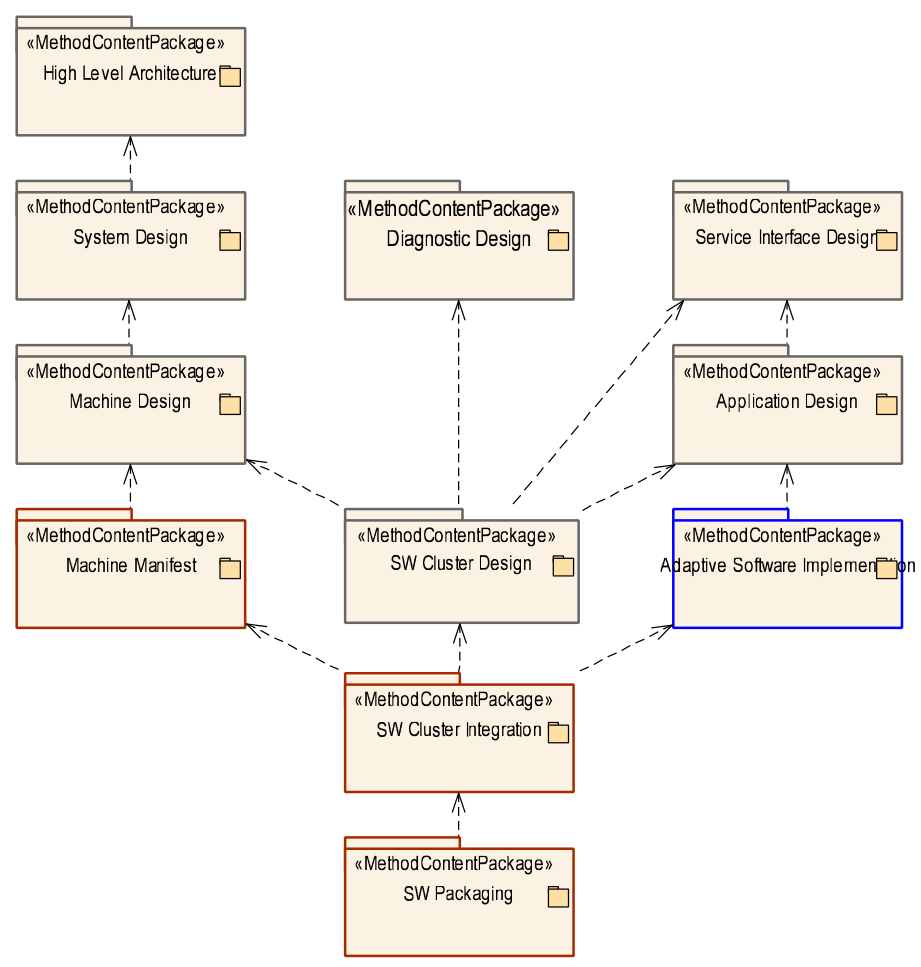
\includegraphics[width=0.75\textwidth]{Images/chap3/image_methodology/knowledgeBase/AdaptiveMethodology.png}
    \vspace{0.5cm}
    \caption{Adaptive Methodology}
    \label{fig:adap_methodology}
\end{figure}

% \subsubsection{High Level Architecture}

% % Figure before explanation
% \begin{figure}[H] % Dùng ht (here, top) là chuẩn nhất
%     \centering
%     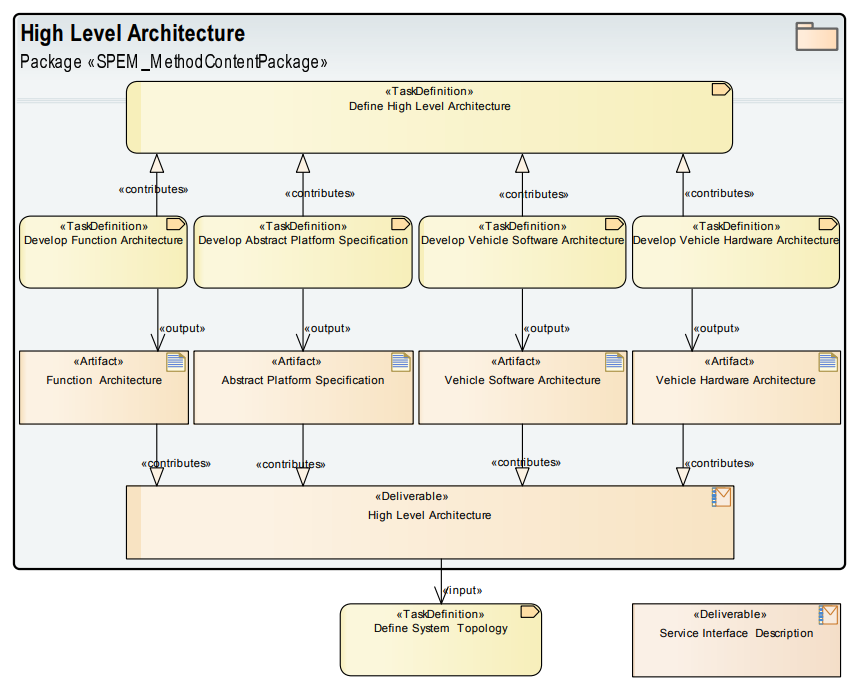
\includegraphics[width=0.75\textwidth]{Images/chap3/image_methodology/knowledgeBase/HLA.png}
%     \vspace{0.5cm}
%     \caption{High Level Architecture in Adaptive AUTOSAR Methodology}
%     \label{fig:hla_architecture} % Đã đổi tên nhãn để không trùng
% \end{figure}

% The High Level Architecture represents the initial and most abstract architectural view within the Adaptive AUTOSAR Methodology. Its primary purpose is to establish a common architectural foundation for the vehicle E/E system before detailed system design and implementation activities are performed.

% As illustrated in Figure~\ref{fig:hla_architecture}, the High Level Architecture is defined through a set of coordinated architectural tasks that collectively contribute to a unified architectural deliverable. These tasks include the development of the Function Architecture, the Abstract Platform Specification, the Vehicle Software Architecture, and the Vehicle Hardware Architecture. Each task addresses a specific architectural concern while remaining independent of concrete implementation decisions.

% The Function Architecture focuses on identifying and structuring the system functions and their logical relationships. It describes what the system is expected to do, without specifying how or where these functions are executed. In parallel, the Abstract Platform Specification defines the abstract execution environment and platform capabilities required by the software, serving as a conceptual bridge between functional requirements and platform realization.

% The Vehicle Software Architecture describes the high level organization of software elements within the vehicle, including major software partitions and their responsibilities. Complementarily, the Vehicle Hardware Architecture captures the high-level hardware structure of the system, including computing units and their relationships, without binding the architecture to specific hardware components.

% The outputs of these architectural tasks are formalized as architectural artefacts. These artefacts collectively contribute to the High-Level Architecture deliverable, which serves as a key input for subsequent methodology phases. In particular, the High Level Architecture provides the architectural context required for defining the system topology and service interface descriptions in later stages.

% By separating functional, software, hardware, and platform concerns at this early stage, the High Level Architecture supports architectural clarity, scalability, and consistency. It ensures that subsequent design and integration activities are grounded in a coherent and well-structured architectural vision.


% \subsubsection{System Design}

% % Figure before explanation
% \begin{figure}[H] % Dùng ht (here, top) là chuẩn nhất
%     \centering
%     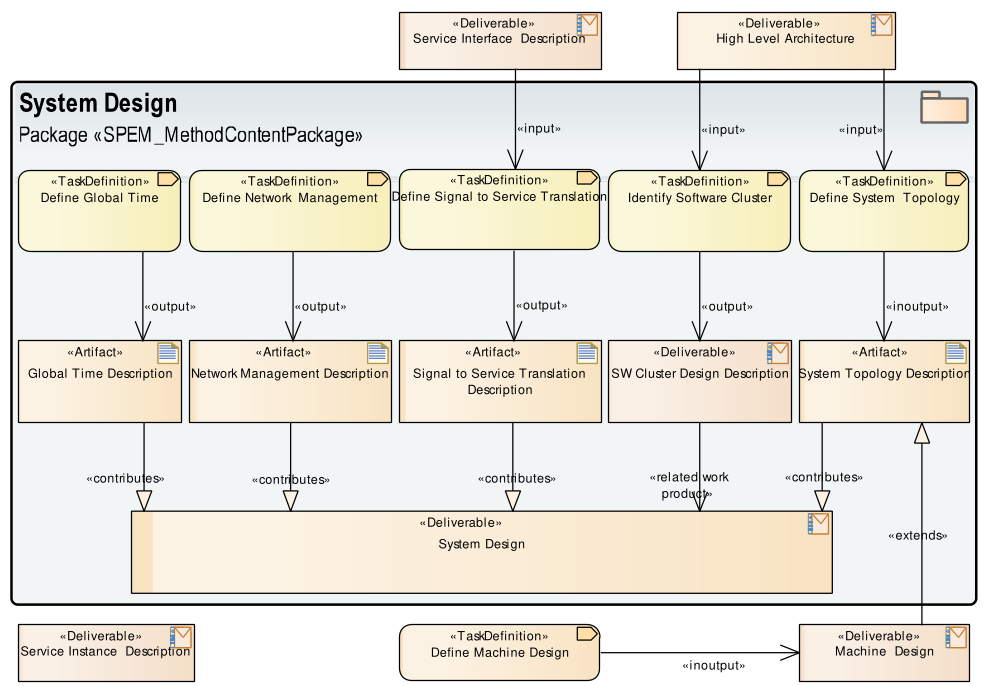
\includegraphics[width=0.75\textwidth]{Images/chap3/image_methodology/knowledgeBase/systemDesign.png}
%     \vspace{0.5cm}
%     \caption{System Design in Adaptive AUTOSAR Methodology}
%     \label{fig:system_design} % Đã đổi tên nhãn để không trùng
% \end{figure}

% The System Design phase refines the architectural concepts established in the High-Level Architecture into a more concrete and structured system-level description. Its primary objective is to define how software elements, communication mechanisms, and system resources are organized and coordinated within the Adaptive AUTOSAR environment.

% As illustrated in the System Design package, this phase consumes key architectural deliverables, including the High Level Architecture and the Service Interface Description, as inputs. Based on these inputs, a set of dedicated design tasks is performed to derive detailed system artefacts that collectively form the System Design deliverable.

% One of the central tasks in this phase is the definition of global timing concepts. The \textit{Define Global Time} task establishes a common time base for the system, which is essential for coordinating distributed software execution and ensuring temporal consistency across different system elements. The resulting Global Time Description contributes to the overall System Design by providing a unified temporal reference.

% In parallel, the \textit{Define Network Management} task specifies how communication networks are controlled and supervised at the system level. This task produces the Network Management Description, which defines network states, transitions, and management strategies. These definitions support reliable communication and controlled system behavior during startup, operation, and shutdown phases.

% Another key task within this phase is the \textit{Define Signal to Service Translation}. This task addresses the mapping between signal-oriented communication and service-oriented communication. The resulting Signal to Service Translation Description enables interaction between system elements that rely on different communication paradigms, ensuring compatibility and interoperability within the Adaptive Platform.

% The System Design phase also includes the identification of software clusters through the \textit{Identify Software Cluster} task. Software clusters group related software elements into coherent deployment units. The resulting Software Cluster Design Description serves as an important intermediate artefact that supports later integration and deployment activities.

% Furthermore, the \textit{Define System Topology} task specifies how system elements are arranged and connected. The System Topology Description captures function groups, network endpoints, and their relationships. This description provides a structural view of the system and serves as a foundation for subsequent deployment and machine-specific design steps.

% All artefacts generated during these tasks contribute to the System Design deliverable. Together, they establish a consistent and detailed system level specification that bridges the gap between high level architectural concepts and later design phases. The System Design deliverable also provides essential inputs for related activities, such as service instance specification and machine design.

% By consolidating timing, communication, clustering, and topology aspects, the System Design phase ensures that the Adaptive AUTOSAR system is coherently structured and ready for further refinement in subsequent methodology stages.


% % TODO: Insert system topology and communication overview figure

% \subsubsection{Service Interface Design}

% % Figure before explanation
% \begin{figure}[H] % Dùng ht (here, top) là chuẩn nhất
%     \centering
%     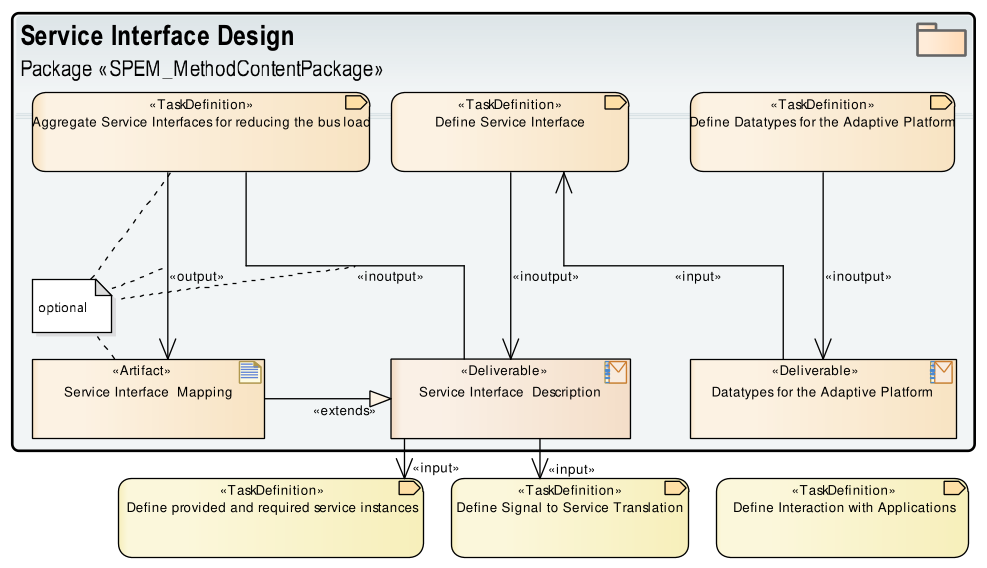
\includegraphics[width=0.75\textwidth]{Images/chap3/image_methodology/knowledgeBase/serviceInterfaceDesign.png}
%     \vspace{0.5cm}
%     \caption{Service Interface Design in Adaptive AUTOSAR Methodology}
%     \label{fig:service_interface_design} % Đã đổi tên nhãn để không trùng
% \end{figure}

% The Service Interface Design defines how Service Interface Descriptions are created, refined, and reused within the Adaptive AUTOSAR development process. This usage scenario explains the sequence of design activities and their associated work products, as illustrated in Figure~\ref{fig:service_interface_design}, focusing on the relationship between service interfaces, datatypes, and interface mappings.

% According to the methodology, Service Interface Descriptions can be obtained through two main usage scenarios: create or change use cases and reuse use cases. These scenarios are not isolated phases but can be integrated into both system design and application design activities, depending on the development context.

% In create or change use cases, Service Interface Descriptions are derived by performing a set of tailored tasks. The central task is the definition of a service interface, which specifies the service operations, events, and communication semantics. In parallel, datatypes for the Adaptive Platform are defined or refined to describe the data exchanged through the service interface. These tasks may be supported by the aggregation of service interfaces, which aims to reduce communication bus load by grouping related service elements when appropriate. The resulting Service Interface Mapping artefact optionally extends the Service Interface Description by documenting how aggregated or related interfaces are organized.

% This scenario is typically applied in a top-down development approach, where architectural or system level considerations drive the definition of service interfaces and datatypes. The outputs of these tasks include the Service Interface Description and the Datatypes for the Adaptive Platform, which together form the primary deliverables of this design stage.

% In reuse use cases, existing Service Interface Descriptions are adopted as inputs with minimal modification. In this case, service interfaces and their associated datatypes are reused from predefined specifications or existing libraries. If required, datatypes may be extended to align with the specific system context. This scenario is commonly applied in a bottom-up development approach and supports efficient reuse across different projects.

% The resulting work products of both scenarios are tailored Service Interface Descriptions and corresponding Datatype Descriptions. These deliverables serve as inputs for subsequent design activities, such as the definition of provided and required service instances, signal-to-service translation, and the specification of interactions with applications.

% By explicitly structuring the creation, aggregation, mapping, and reuse of service interfaces, the Service Interface Design usage scenario ensures consistency, modularity, and reusability of service definitions within the Adaptive AUTOSAR methodology.

% \subsubsection{Application Design}

% % Figure before explanation
% \begin{figure}[H]
%     \centering
%     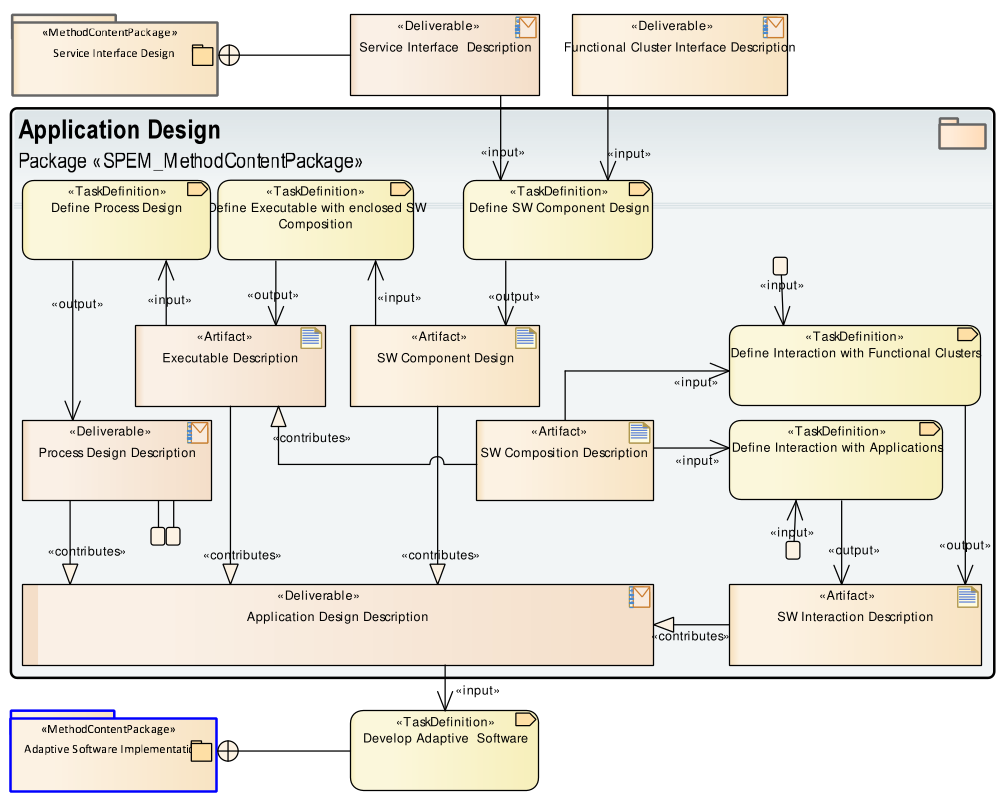
\includegraphics[width=0.75\textwidth]{Images/chap3/image_methodology/knowledgeBase/applicationDesign.png}
%     \vspace{0.5cm}
%     \caption{Application Design in Adaptive AUTOSAR Methodology}
%     \label{fig:application_design}
% \end{figure}

% The Application Design phase refines the outcomes of system level and service-level design into a detailed specification of executable software structures. Its primary objective is to describe how software components are organized, instantiated, and interconnected during runtime execution within the Adaptive AUTOSAR Platform.

% As shown in Figure~\ref{fig:application_design}, this phase takes the Service Interface Description and the Functional Cluster Interface Description as inputs. Based on these artefacts, a set of closely related design activities is carried out, leading to the definition of the overall Application Design Description.

% One of the key activities in this phase is \textit{Define Software (SW) Component Design}. This activity results in the SW Component Design artefact, which specifies the internal structure of software components and their interaction endpoints. These endpoints are expressed through software component (SWC) ports instantiating specific port interfaces at either the application level or the platform level. The SW Component Design establishes the structural basis required for subsequent composition and interaction definitions.

% Another essential activity is \textit{Define Executable with enclosed SW Composition}, which determines how software components are assembled into executable units. Its outcome is the Executable Description, including the SW Composition Description. This description identifies the software components contained within an executable and defines their structural relationships. The execution of this activity requires that all referenced SW Component Designs are already available.

% The runtime realization of executables is addressed by the \textit{Define Process Design} activity. The resulting Process Design Description represents a design time abstraction of the operating system process responsible for instantiating and starting a specific executable. This activity builds upon the Executable Description and provides the link between executable definitions and their runtime execution context.

% Interaction which related aspects are specified through the activities \textit{Define Interaction with Applications} and \textit{Define Interaction with Functional Clusters}. Together, these activities produce the SW Interaction Description, which captures all interaction configurations that are relevant at design time. This includes interactions between application-level software components as well as interactions with platform-level functional clusters. The definition of these interactions depends on the availability of the Process Design Description, the corresponding Executable Description with its SW Composition Description, and the interaction endpoints defined in the SW Component Designs.

% All artefacts produced during the Application Design phase contribute to the Application Design Description deliverable. This deliverable consolidates software component definitions, executable compositions, process abstractions, and interaction configurations into a consistent and comprehensive design representation.

% The activities within the Application Design phase are interdependent and may be performed in an order that best fits the project context. Although the primary focus of this phase is on application-level software, the same design principles and activities may also be applied to platform-level software, particularly when port and port interface concepts are supported.

% The resulting Application Design Description serves as a fundamental input for the subsequent Adaptive Software Implementation phase, where the defined software structures are realized as executable software.

% \subsubsection{Adaptive Software Implementation}

% % Figure before explanation
% \begin{figure}[H]
%     \centering
%     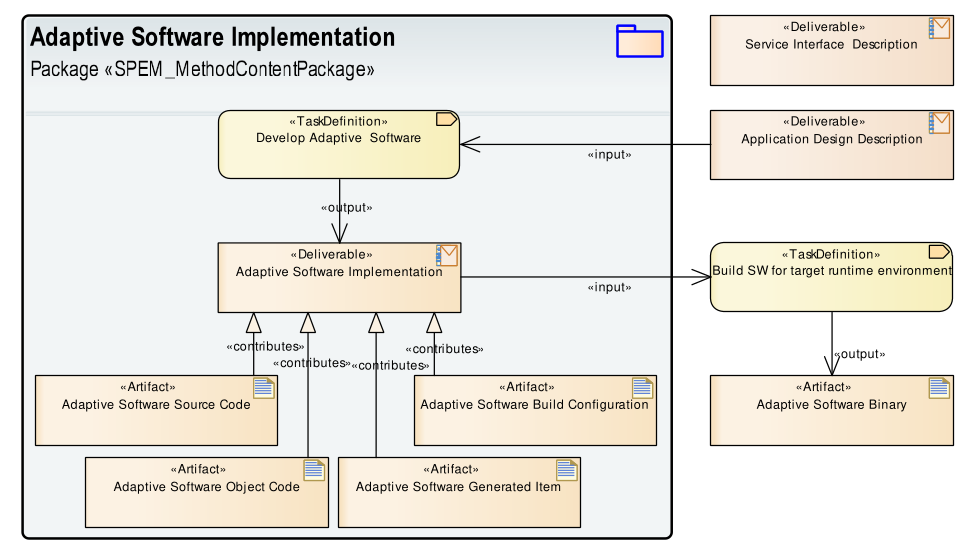
\includegraphics[width=0.75\textwidth]{Images/chap3/image_methodology/knowledgeBase/softwareImplementation.png}
%     \vspace{0.5cm}
%     \caption{Adaptive Software Implementation in Adaptive AUTOSAR Methodology}
%     \label{fig:software_implementation}
% \end{figure}

% The Adaptive Software Implementation phase addresses the realization of software defined during the preceding design stages. Its purpose is to transform the Application Design Description into concrete software artefacts that can be integrated and executed within the Adaptive AUTOSAR runtime environment.

% As depicted in Figure~\ref{fig:software_implementation}, this phase is initiated once the Service Interface Description and the Application Design Description are available. These deliverables provide the necessary interface definitions and structural specifications required to start the implementation activities.

% The central activity of this phase is \textit{Develop Adaptive Software}. This activity encompasses the development of application level and/or platform level Adaptive Software and may include analysis, detailed design, implementation, and testing activities. The development process relies on Adaptive Software Generated Items, such as service proxies and service skeletons, which are derived from service interface definitions and support the implementation of communication ports and port interfaces.

% Depending on the availability of the Adaptive Software Build Configuration, the development process follows different realization paths. When the build configuration is known in advance, software components can be compiled by the developer, and Adaptive Software Object Code can be delivered directly. In contrast, if the build configuration is not available, the developer provides Adaptive Software Source Code, and the compilation is performed later by the integrator.

% The artefacts produced during software development include Adaptive Software Source Code, Adaptive Software Object Code, Adaptive Software Generated Items, and the Adaptive Software Build Configuration. Together, these artefacts contribute to the Adaptive Software Implementation deliverable, which represents the complete implementation result prepared for integration.

% The transformation of the implementation into deployable form is addressed by the activity \textit{Build software (SW) for target runtime environment}. This activity consumes the Adaptive Software Implementation and produces the Adaptive Software Binary. The binary represents the executable form of the software that is suitable for deployment on the target machine and runtime environment.

% Throughout this phase, both application level and platform level Adaptive Software are treated consistently. Each executable requires a main function and an execution manifest, enabling instantiation and deployment within the Adaptive AUTOSAR execution framework.

% The Adaptive Software Implementation deliverable produced in this phase serves as the handover point between software development and integration. It provides the necessary implementation artefacts for subsequent software cluster integration, packaging, and deployment activities.

% \subsubsection{Diagnostic Design}

% % Figure before explanation
% \begin{figure}[H]
%     \centering
%     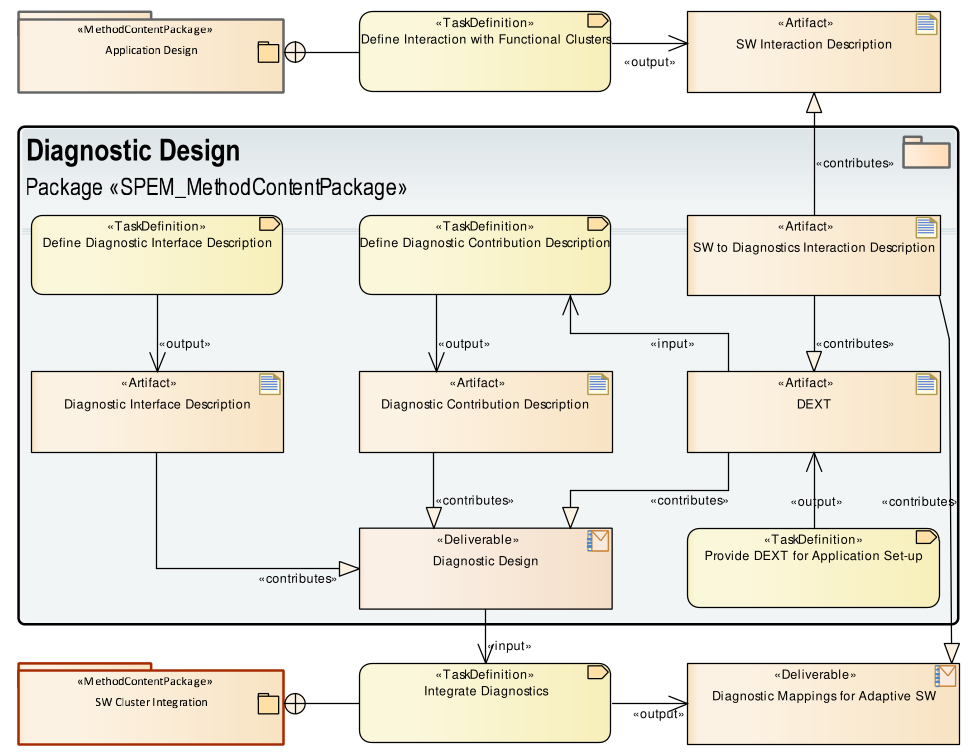
\includegraphics[width=0.75\textwidth]{Images/chap3/image_methodology/knowledgeBase/diagDesign.png}
%     \vspace{0.5cm}
%     \caption{Diagnostic Design in Adaptive AUTOSAR Methodology}
%     \label{fig:diag_design}
% \end{figure}

% The Diagnostic Design phase focuses on defining how diagnostic information is associated with the software structures of the Adaptive AUTOSAR system. Its main objective is to prepare diagnostic which related artefacts that enable consistent monitoring, reporting, and interaction with the diagnostic manager during system operation.

% As shown in Figure~\ref{fig:diag_design}, Diagnostic Design builds on results obtained during the Application Design phase, particularly the SW Interaction Description that captures interactions with functional clusters. These interaction definitions provide the context required to specify diagnostic interfaces and mappings in a systematic manner.

% The activity \textit{Define Diagnostic Interface Description} establishes the diagnostic interfaces that adaptive software components expose for diagnostic purposes. The resulting Diagnostic Interface Description specifies diagnostic port interfaces and their characteristics, allowing diagnostic managers to access diagnostic which relevant data and services in a standardized way.

% Complementing this, the activity \textit{Define Diagnostic Contribution Description} identifies the diagnostic content contributed by software elements within a given context. The Diagnostic Contribution Description determines which parts of the diagnostic configuration are relevant for specific executables or software clusters and are intended to be processed by the diagnostic manager.

% Diagnostic resources and configuration data are collected and structured through the activity \textit{Provide DEXT for Application Setup}. This activity produces or extends the Diagnostic Extract (DEXT), which contains diagnostic resources such as diagnostic data identifiers, diagnostic events, enable conditions, and operation cycles. The DEXT acts as a reusable container for diagnostic configuration and may cover multiple executables, diagnostic managers, and software clusters across the vehicle.

% The association between diagnostic resources and software interaction endpoints is captured in the SW to Diagnostics Interaction Description. This artefact specifies how diagnostic information is mapped to software component ports at design time and contributes both to the Diagnostic Design deliverable and to the DEXT. It represents an intermediate form of diagnostic mappings that is refined during later integration steps.

% All artefacts produced during this phase, including the Diagnostic Interface Description, Diagnostic Contribution Description, SW to Diagnostics Interaction Description, and the DEXT, collectively contribute to the Diagnostic Design deliverable. This deliverable provides a consolidated view of the diagnostic configuration that is prepared for further integration activities.

% The Diagnostic Design deliverable is subsequently used as input for the \textit{Integrate Diagnostics} activity during Software Cluster Integration. In that phase, diagnostic mappings are finalized by associating diagnostic resources with concrete executable instances and operating system processes, resulting in the Diagnostic Mappings for Adaptive Software.

% By structuring diagnostic interface definition, contribution specification, and resource extraction as distinct but related activities, the Diagnostic Design phase supports a clear and maintainable diagnostic configuration process within the Adaptive AUTOSAR methodology.

% \subsubsection{Machine Design}

% % Figure before explanation
% \begin{figure}[H]
%     \centering
%     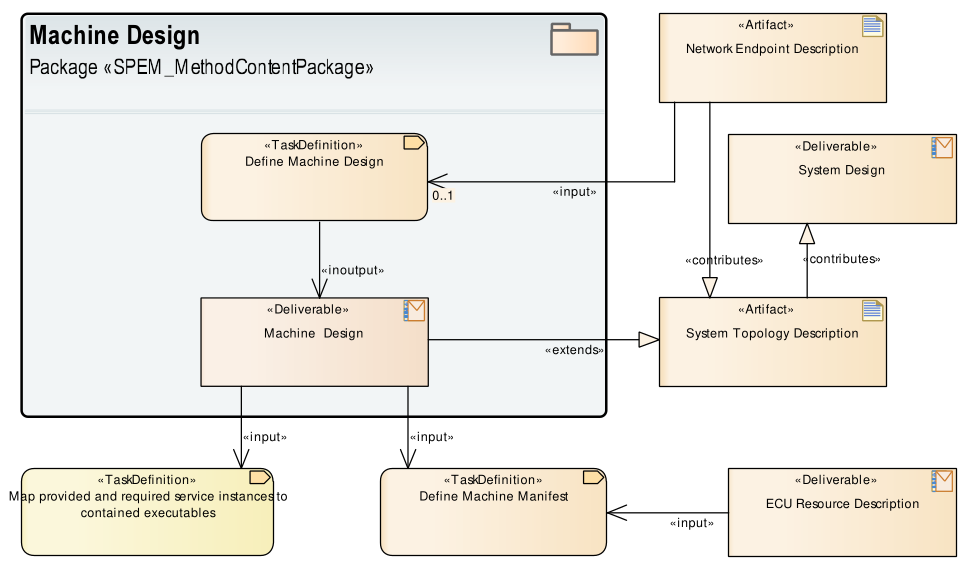
\includegraphics[width=0.75\textwidth]{Images/chap3/image_methodology/knowledgeBase/machineDesign.png}
%     \vspace{0.5cm}
%     \caption{Machine Design in Adaptive AUTOSAR Methodology}
%     \label{fig:machine_design}
% \end{figure}

% The Machine Design phase addresses the specification of a machine from a communication and deployment standpoint within the Adaptive AUTOSAR Platform. Its aim is to describe the characteristics of a machine that are required for software execution and service communication, taking into account system level topology information and the capabilities of the target ECU.

% Figure~\ref{fig:machine_design} provides an overview of the activities involved in this phase. The core activity, \textit{Define Machine Design}, derives a machine-oriented configuration by using network endpoint information defined during System Design. In particular, the System Topology Description and the associated Network Endpoint Description supply the addressing and service discovery parameters needed to shape the communication behavior of the machine.

% The result of this activity is captured in the Machine Design deliverable. This deliverable augments the existing System Topology Description by introducing machine specific communication constraints and requirements. At this stage, the design remains independent of a concrete hardware realization and represents a prospective configuration for a machine.

% Beyond defining communication aspects, the Machine Design also provides the basis for associating software deployment elements with the machine. Through the activity \textit{Map provided and required service instances to contained executables}, service instances are linked to executables that are intended to run on the machine. This association clarifies how services are realized by software units within the machine context.

% The adaptation of the machine configuration to a specific hardware platform is performed in a subsequent activity, \textit{Define Machine Manifest}. This activity combines the Machine Design with the ECU Resource Description, which details the resources and limitations of the target ECU. The outcome is the Machine Manifest, representing a machine configuration that is fully aligned with the characteristics of a real ECU.

% From a methodological viewpoint, machine configuration follows a two-step process. The first step establishes the communication structure of a machine and yields the Machine Design. This step may be carried out in a top-down manner, guided by an existing System Design, or in a bottom-up manner, where machine-specific communication definitions are created locally and may later contribute to the overall system topology.

% The second step focuses on hardware-specific realization and results in the Machine Manifest. This separation between prospective machine definition and ECU specific configuration supports a clear allocation of responsibilities between system designers and integrators, while maintaining flexibility during system integration.

% \subsubsection{Machine Manifest}

% % Figure before explanation
% \begin{figure}[H]
%     \centering
%     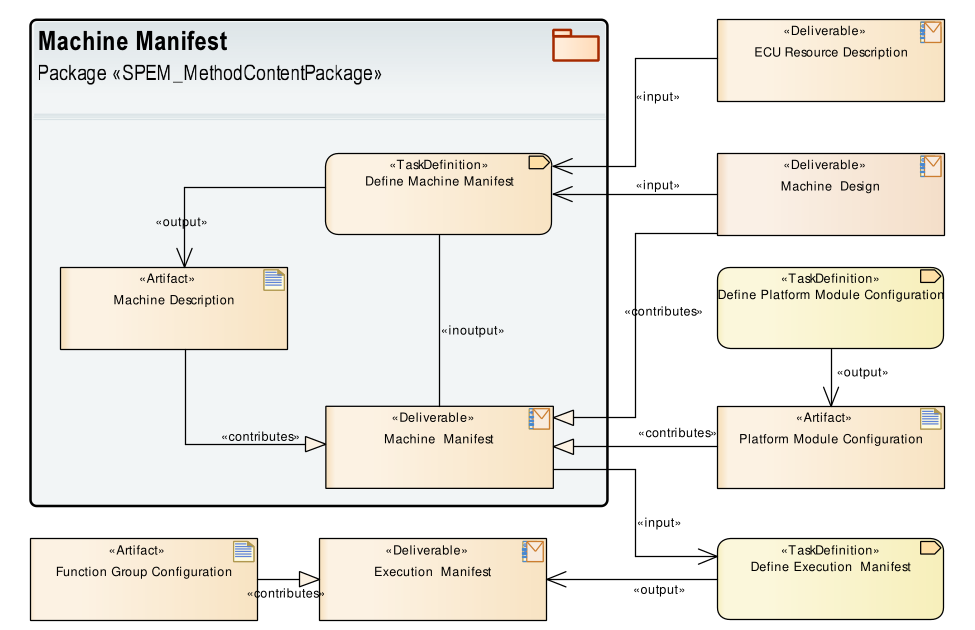
\includegraphics[width=0.75\textwidth]{Images/chap3/image_methodology/knowledgeBase/machineManifest.png}
%     \vspace{0.5cm}
%     \caption{Machine Manifest in Adaptive AUTOSAR Methodology}
%     \label{fig:machine_manifest}
% \end{figure}

% The Machine Manifest phase specifies the final configuration of a machine that is ready to be deployed on a concrete ECU within the Adaptive AUTOSAR Platform. Its purpose is to consolidate communication-related design results with hardware resource information and platform-specific configurations into a single, deployment ready description.

% Figure~\ref{fig:machine_manifest} outlines the activities and work products involved in this phase. The primary activity, \textit{Define Machine Manifest}, is initiated once the Machine Design and the ECU Resource Description are available. While the Machine Design provides a prospective view of the machine configuration, the ECU Resource Description defines the concrete hardware resources offered by the target ECU.

% The outcome of this activity is the Machine Manifest deliverable. The Machine Manifest integrates several key elements. First, it contains the Machine Description, which describes the available hardware resources of the ECU, such as processing units, memory resources, sensors, actuators, and other relevant hardware elements. This information is derived from the ECU Resource Description and tailored to the specific machine instance.

% Second, the Machine Manifest incorporates the Machine Design, thereby preserving the communication structure and network-related configuration that was defined during the Machine Design phase. This ensures that the communication requirements identified earlier are consistently realized on the target ECU.

% In addition, platform-specific aspects are addressed through the activity \textit{Define Platform Module Configuration}. This activity produces Platform Module Configuration artefacts, which specify the machine-specific configuration of Adaptive Platform modules. These configurations may include the operating system setup, platform services such as network management and diagnostics, as well as foundation modules like logging and tracing. The resulting Platform Module Configurations contribute directly to the Machine Manifest.

% The configuration of software execution is captured by the activity \textit{Define Execution Manifest}. This activity produces the Execution Manifest, which specifies which executables are instantiated on the machine and how they are mapped to processes. The Execution Manifest may also include Function Group Configurations that control the activation and deactivation of software elements. The Execution Manifest contributes to the Machine Manifest by defining the runtime behavior of software on the machine.

% From a process perspective, the Machine Manifest is typically assembled in an incremental manner. Communication-related configurations originating from the Machine Design are collected first, followed by the integration of hardware resource descriptions and platform module configurations. As additional configuration information becomes available, the Machine Manifest may be iteratively extended and refined.

% By consolidating machine-specific communication settings, hardware resource descriptions, platform module configurations, and execution information, the Machine Manifest provides a complete and consistent representation of a machine that is ready for deployment within the Adaptive AUTOSAR ecosystem.

% \subsubsection{Software Cluster Design, Integration, and Packaging}

% The phases of Software Cluster Design, Software Cluster Integration, and Software Packaging together form the final preparation steps that transform implemented Adaptive AUTOSAR software into deployable units. These phases consolidate design results, integrate software components with their configurations, and prepare complete software packages for deployment on target machines.

% Software Cluster Design focuses on defining logical groupings of software elements that belong together from a deployment and lifecycle perspective. A software cluster typically bundles application level software, required platform services, and related configuration artifacts into a coherent unit. The purpose of this phase is not to define execution details, but to establish clear cluster boundaries, dependencies, and responsibilities that simplify later integration and deployment activities.

% Based on the cluster definitions, Software Cluster Integration performs the concrete assembly of software and configuration artifacts. During this phase, Adaptive Software Implementations, design descriptions, machine which related information, and diagnostic configurations are brought together and checked for consistency. Integration activities refine execution which related information, such as the association of executables with machines and processes, and complete interaction and diagnostic mappings that could only be finalized once all involved elements are known. As a result, the integrated software cluster represents a consistent and executable view of the system for a specific deployment context.

% Software Packaging completes the workflow by preparing integrated software clusters for delivery and deployment. In this phase, all relevant artifacts, such as software binaries, manifests, configuration files and generated items which are collected and organized into software packages. These packages are structured in a way that supports deployment, update, and lifecycle management, while preserving a clear separation between different software clusters.

% By combining cluster definition, integration, and packaging into a structured workflow, these phases provide a clear transition from implemented software to deployable units. This approach supports modularity, reuse, and scalable integration, which are essential characteristics of the Adaptive AUTOSAR methodology.

% \subsubsection{Summary}

% This section has presented an overview of the Adaptive AUTOSAR knowledge base and its role in structuring the development of complex automotive software systems. The methodology defines a clear sequence of development phases, each supported by well-defined artefacts and responsibilities.

Starting from high-level architectural descriptions, the methodology guides the refinement of system structure, service interfaces, application design, and software implementation. Subsequent phases address diagnostics, machine-specific configuration, and the preparation of software for deployment. Each phase builds upon the results of previous stages, ensuring consistency and traceability throughout the development process.

By explicitly modeling artefact dependencies and separating design, implementation, integration, and deployment concerns, the Adaptive AUTOSAR Methodology supports systematic system development. This approach improves scalability, facilitates reuse, and simplifies integration in large and evolving software systems.

The following section explains how the most important Method Content Packages are configured in this project and how they are refined into concrete Adaptive AUTOSAR artefacts.

% Overall, the knowledge base provides a solid methodological foundation for configuring and deploying Adaptive AUTOSAR systems. It enables a structured transition from abstract system concepts to deployable software units while maintaining clarity and consistency across the entire system lifecycle.


\subsection{Project Methodology}

In this project, the Adaptive AUTOSAR system is developed using the \texttt{Autosar.io} tool provided by PopcornSAR. Autosar.io is a configuration-oriented modeling environment that allows users to systematically define and organize an Adaptive AUTOSAR project through a set of well-structured design sections. Instead of focusing on source code implementation, the tool guides users to configure machines, services, and applications by following the standard Adaptive AUTOSAR modeling workflow.

\begin{figure}[H]
    \centering
    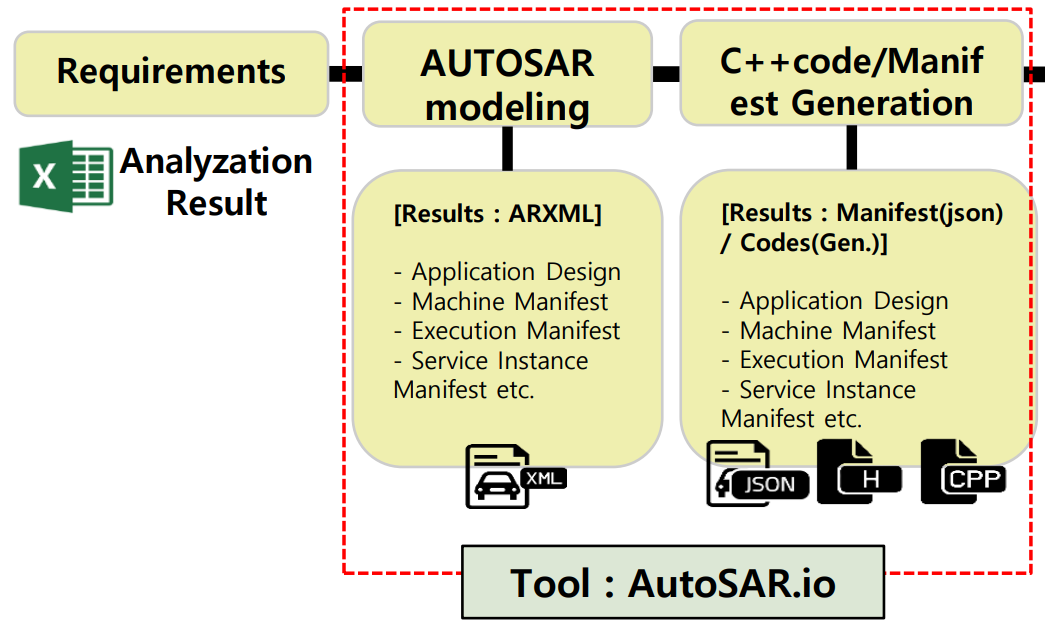
\includegraphics[width=0.75\textwidth]{Images/toolchains/autosario.png}
    \vspace{0.5cm}
    \caption{Autosar.io tool supporting configuration workflow for Adaptive AUTOSAR systems}
    \label{fig:autosario}
\end{figure}

Autosar.io provides dedicated design views that correspond directly to the configuration steps presented in this section, including Machine Design and Machine Manifest creation, Service Interface Design and Mapping, and Adaptive Application Design. Through these views, users can specify network endpoints, service discovery parameters, service interfaces, service instances, application executables, processes, startup behavior, and process-to-machine mappings. Each configuration step produces AUTOSAR-compliant artifacts such as ARXML descriptions and manifests, ensuring consistency between design intent and deployment configuration.

By using Autosar.io, users can incrementally build the system configuration in a top-down manner, where abstract architectural decisions are progressively refined into concrete runtime configurations. This approach enables clear separation between machine-level configuration, service-level communication design, and application-level deployment. As demonstrated throughout this section, Autosar.io acts as the central tool that connects all configuration stages, allowing users to define a complete Adaptive AUTOSAR system in a structured, traceable, and standardized way before moving to implementation and integration phases.

%introduce Autosar.io tool, this is a tool help configuring project based on Adaptive AUTOSAR
\subsubsection{High Level Architecture}
\begin{figure}[H]
    \centering
    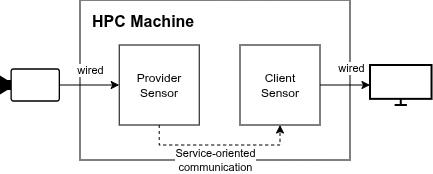
\includegraphics[width=0.75\textwidth]{Images/chap3/image_methodology/machineDesign/high_level.png}
    \vspace{0.5cm}
    \caption{High Level Architecture of Prototype Project}
    \label{fig:hla_project}
\end{figure}

Based on the defined high-level architecture, the Adaptive AUTOSAR configuration process is carried out in a stepwise manner, following the recommended methodology. The overall system design is progressively refined from an abstract architectural view to concrete deployment and execution artifacts.

First, the Machine Design and Machine Manifest are configured to define the physical execution environment of the system. This step specifies the target machine, network interfaces, service discovery settings, operating system platform modules, and lifecycle-related parameters, forming the foundation on which all applications and services are deployed.

Next, the Service Interface Design and Mapping phase focuses on defining the service-oriented communication between applications. During this stage, data types, service interfaces, service instances, and deployment configurations are specified, and abstract service definitions are bound to concrete network endpoints. This step enables standardized and loosely coupled interaction between the Provider Sensor and Client Sensor.

Finally, the Application Design phase models the adaptive applications themselves. Executables are defined and configured, ports are mapped to service interfaces, application processes are created, and startup and lifecycle behaviors are specified. Through this step, the logical application design is concretely mapped onto the target machine, completing the system configuration prior to code and manifest generation.

\subsubsection{Machine Design and Machine Manifest}

% Define Ethernet network endpoint
\begin{figure}[H]
    \centering
    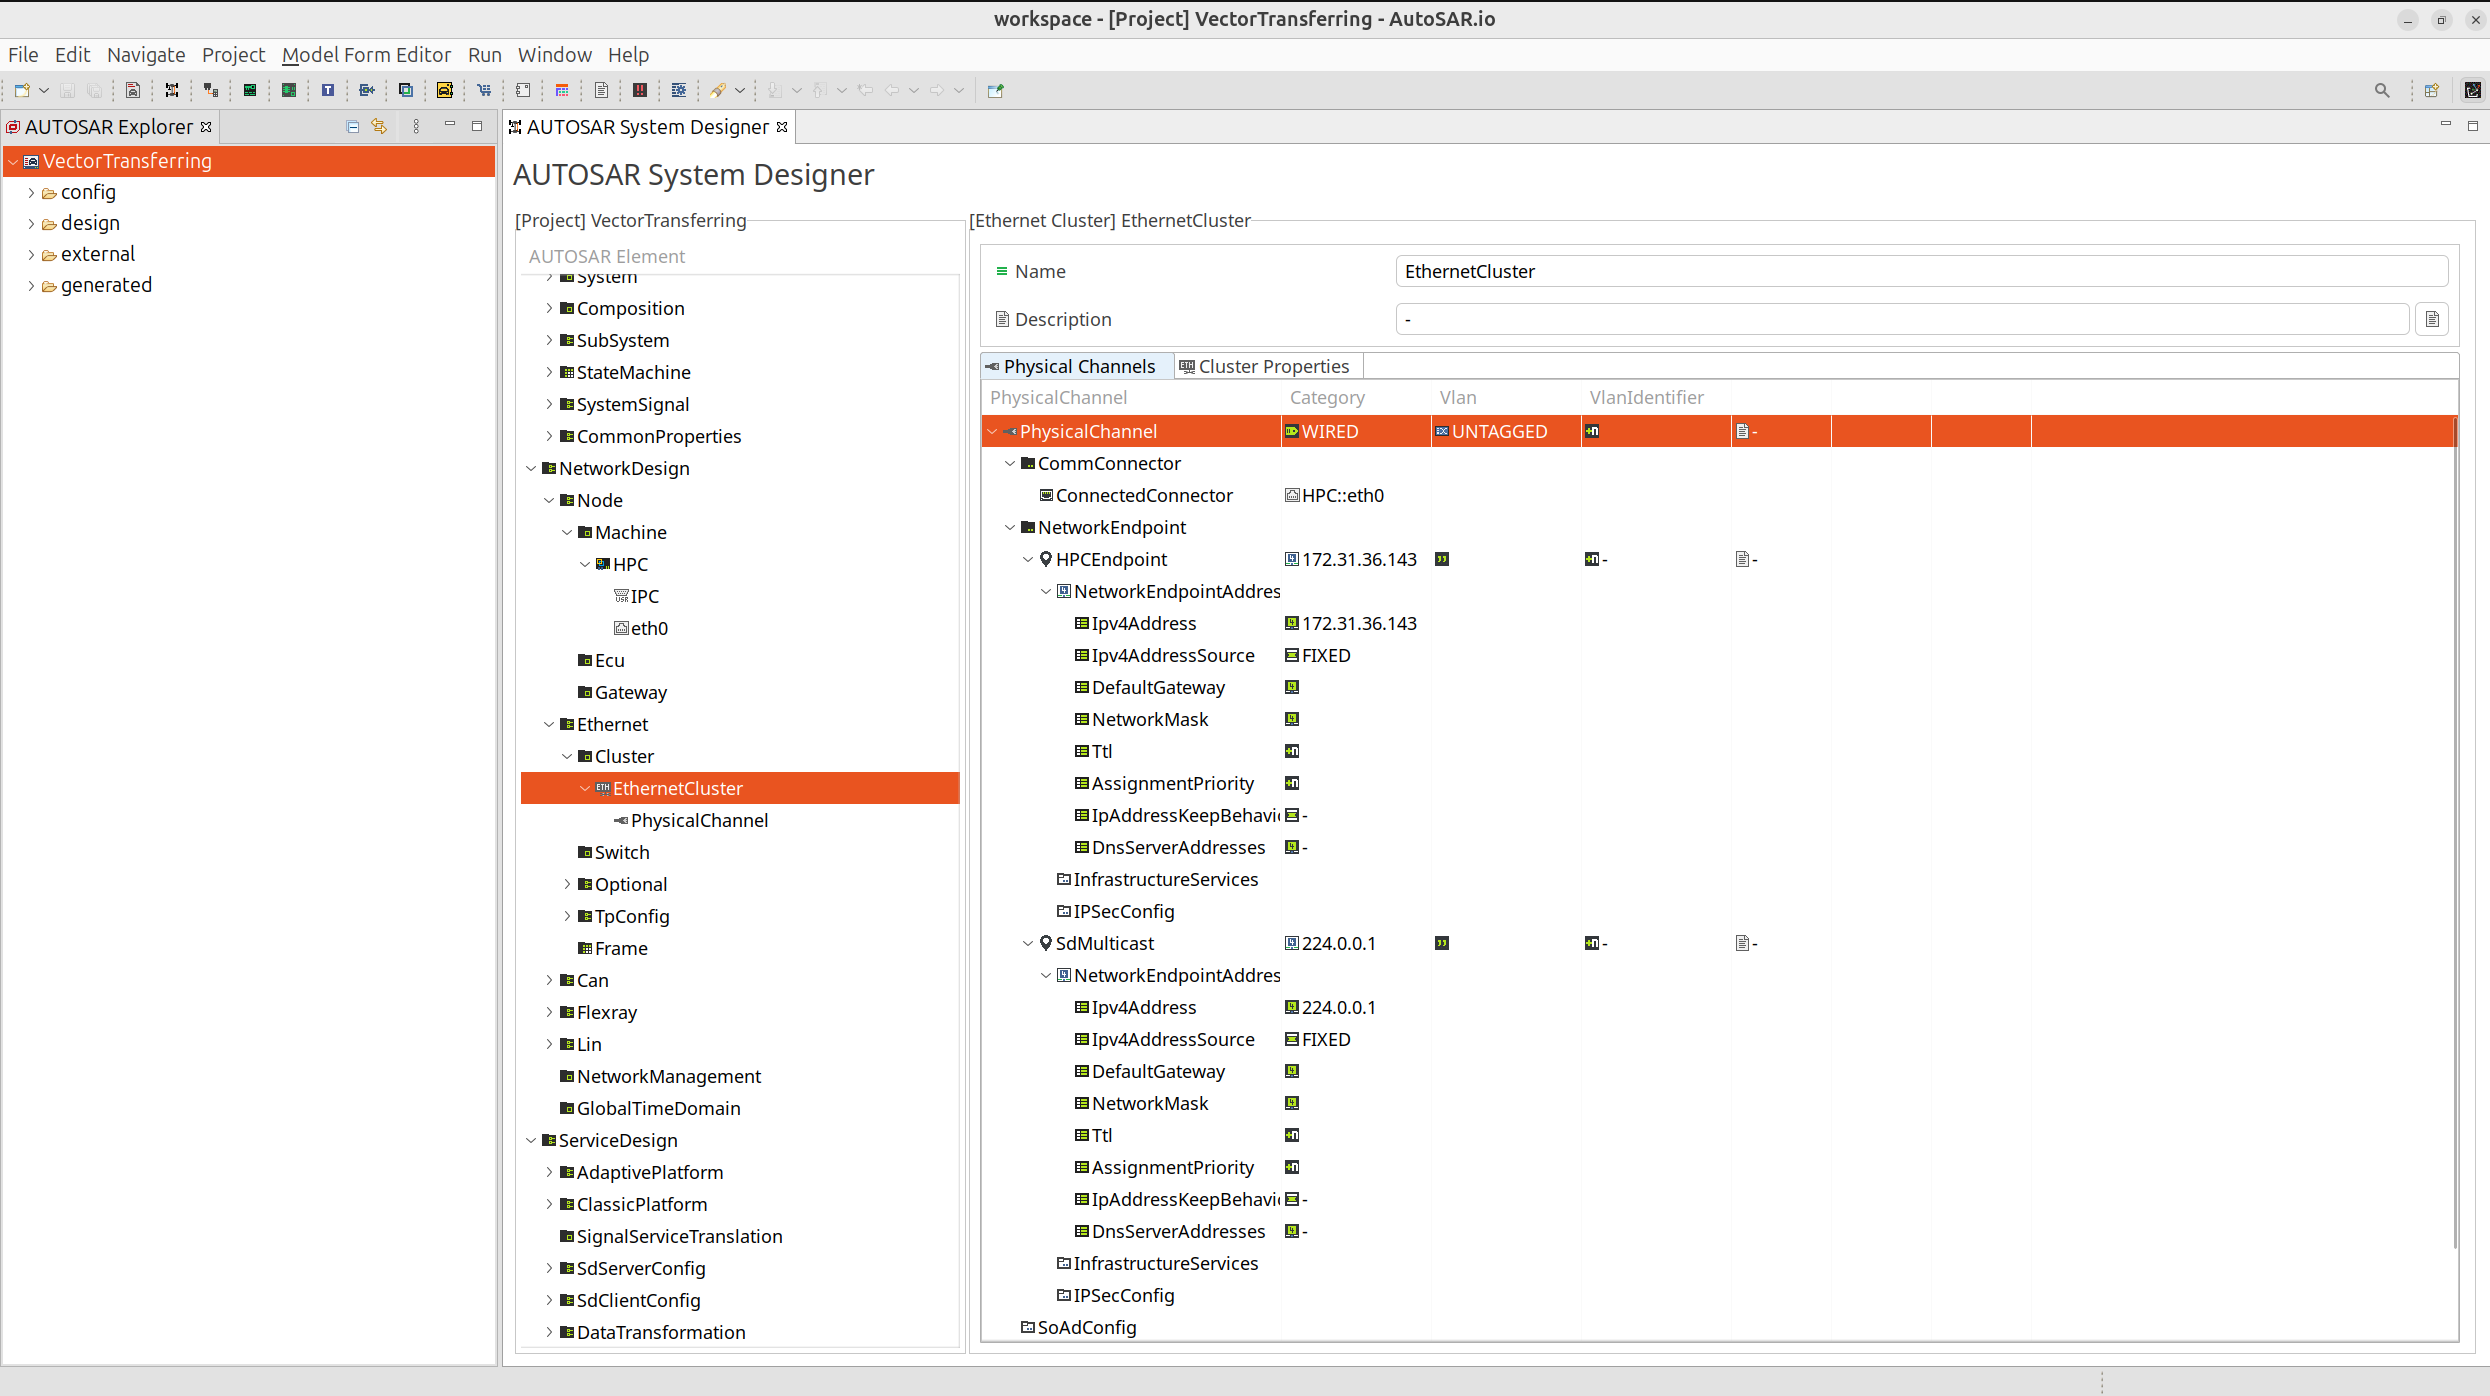
\includegraphics[width=0.75\textwidth]{Images/chap3/image_methodology/machineDesign/defineEthernet.png}
    \vspace{0.5cm}
    \caption{Definition of Ethernet Network Endpoint in Machine Design}
    \label{fig:machine_define_ethernet}
\end{figure}

Figure~\ref{fig:machine_define_ethernet} illustrates the detailed configuration of an Ethernet network endpoint within the AUTOSAR System Designer. An EthernetCluster is defined with a wired physical channel, where the VLAN mode is set to untagged, indicating that no VLAN identifier is applied to the network traffic. The machine node labeled HPC is connected to this cluster through the communication connector HPC eth0, which represents the physical Ethernet interface of the target machine.

The network endpoint configuration specifies a fixed IPv4 address of 172.31.36.143, with the address source explicitly defined as fixed to ensure deterministic network behavior. In addition to the unicast endpoint, a multicast configuration is also present using the IPv4 address 224.0.0.1, which is commonly used for service discovery communication. These settings collectively define how the machine participates in both point to point and multicast Ethernet communication, forming a stable networking foundation for Adaptive AUTOSAR service based applications.

% Add Ethernet configuration to Machine Design
\begin{figure}[H]
    \centering
    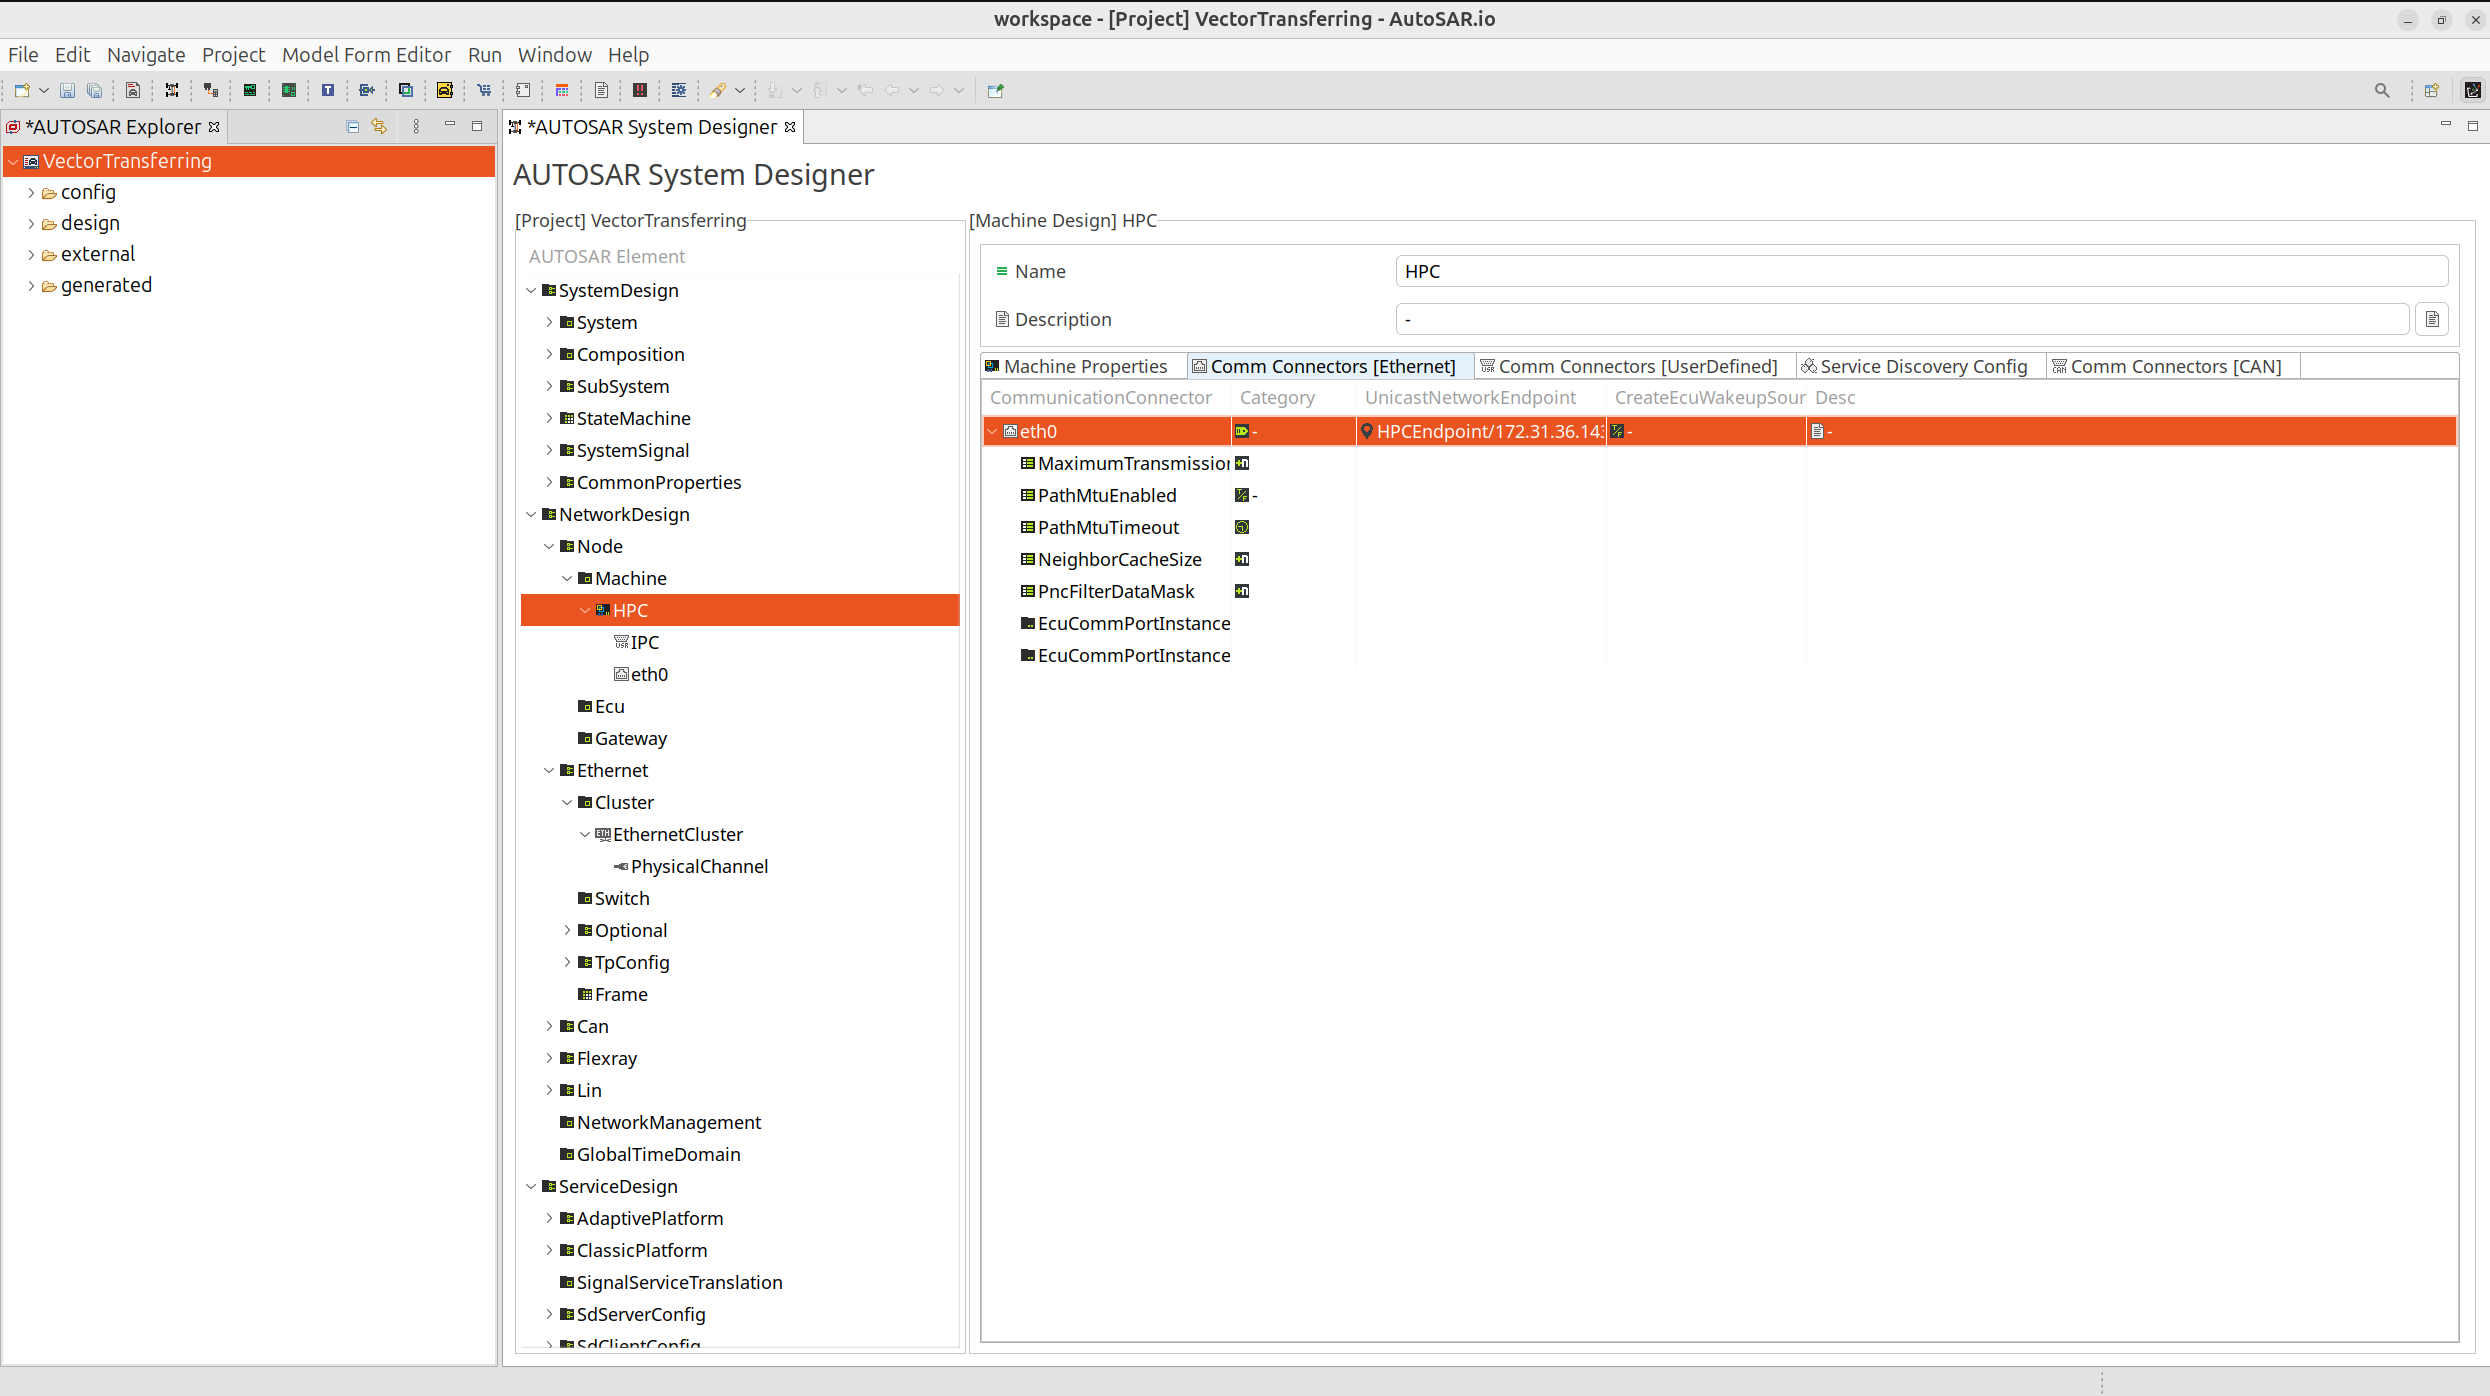
\includegraphics[width=0.75\textwidth]{Images/chap3/image_methodology/machineDesign/addEthMachineDesign.png}
    \vspace{0.5cm}
    \caption{Integration of Ethernet Configuration into Machine Design}
    \label{fig:machine_add_eth_design}
\end{figure}

Figure~\ref{fig:machine_add_eth_design} depicts how the HPC machine is linked to its network interface through the eth0 connector in the Machine Design view. This connector is mapped to a unicast endpoint identified as HPCEndpoint with the IPv4 address 172.31.36.143, defining the machine’s network presence within the Adaptive AUTOSAR system. The figure also highlights adjustable communication parameters such as transmission limits and path MTU handling, which allow the network behavior to be adapted while maintaining reliable data exchange at runtime.

% Configure Service Discovery in Machine Design
\begin{figure}[H]
    \centering
    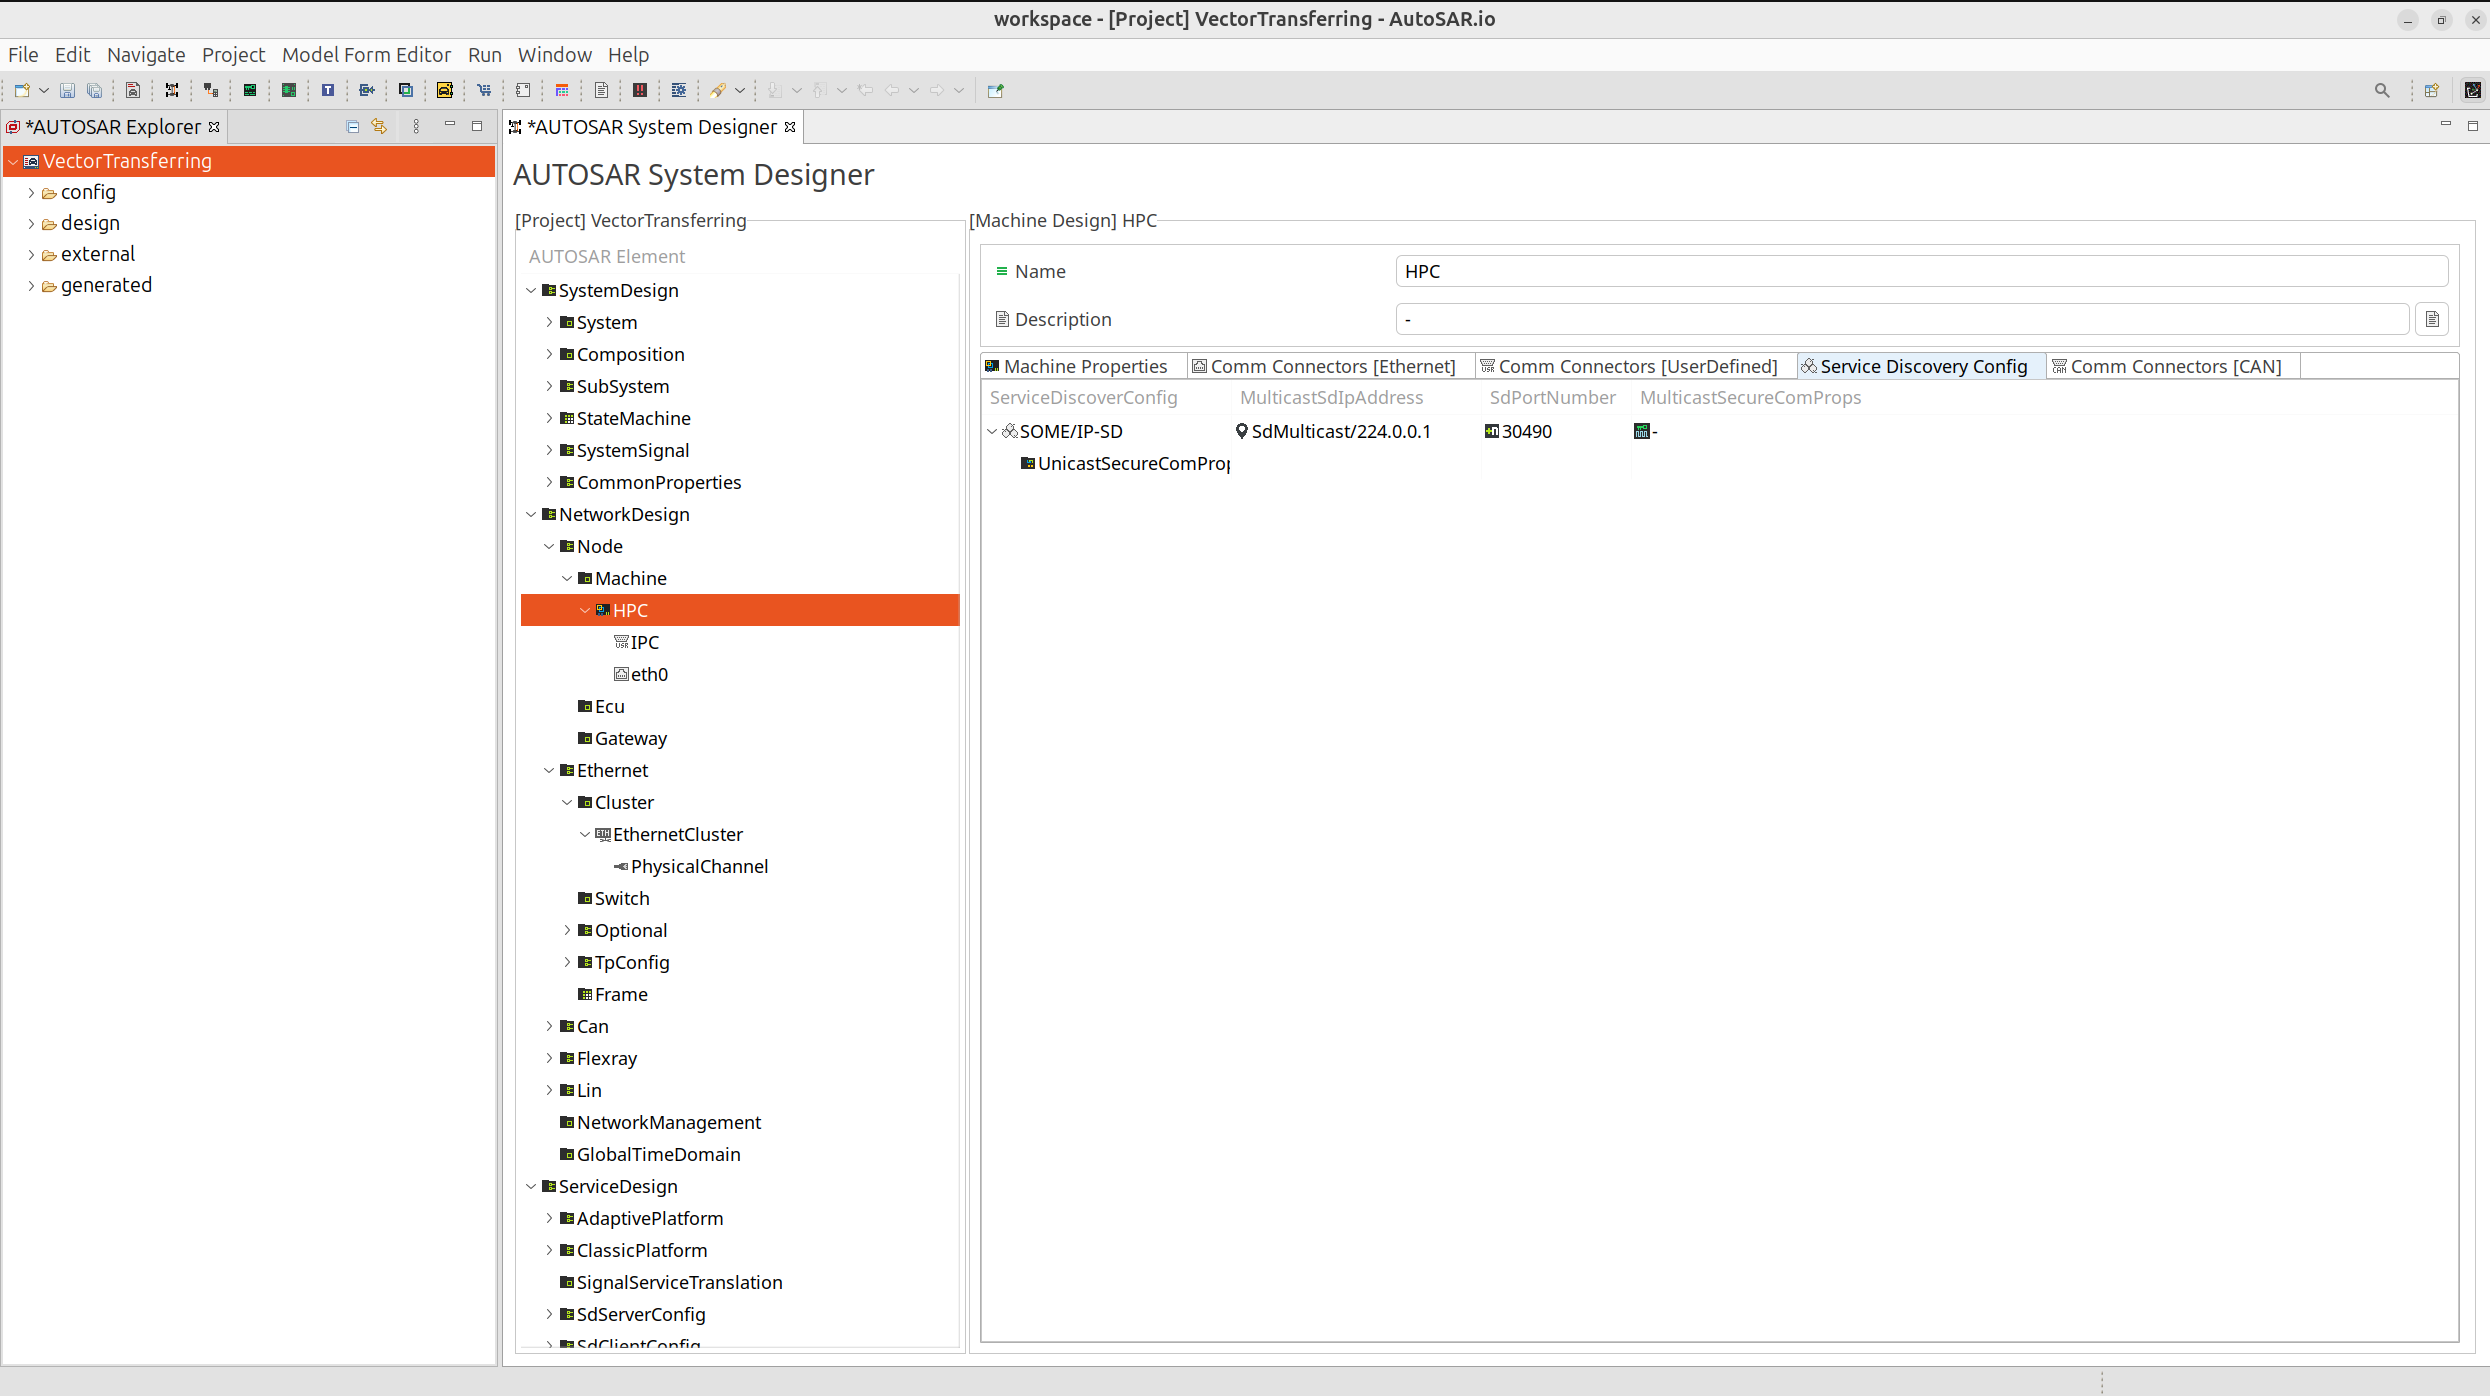
\includegraphics[width=0.75\textwidth]{Images/chap3/image_methodology/machineDesign/addSdConfigMachineDesign.png}
    \vspace{0.5cm}
    \caption{Service Discovery Configuration in Machine Design}
    \label{fig:machine_sd_config}
\end{figure}

Figure~\ref{fig:machine_sd_config} illustrates the Service Discovery setup for the HPC machine within the Machine Design environment. The SOME IP Service Discovery mechanism is configured using the multicast address 224.0.0.1 together with the service discovery port number 30490, which enables applications to announce and detect available services at runtime. This configuration allows dynamic interaction between Adaptive AUTOSAR applications while supporting flexible service availability without relying on static communication bindings.

% Configure Diagnostic Log and Trace (DLT)
\begin{figure}[H]
    \centering
    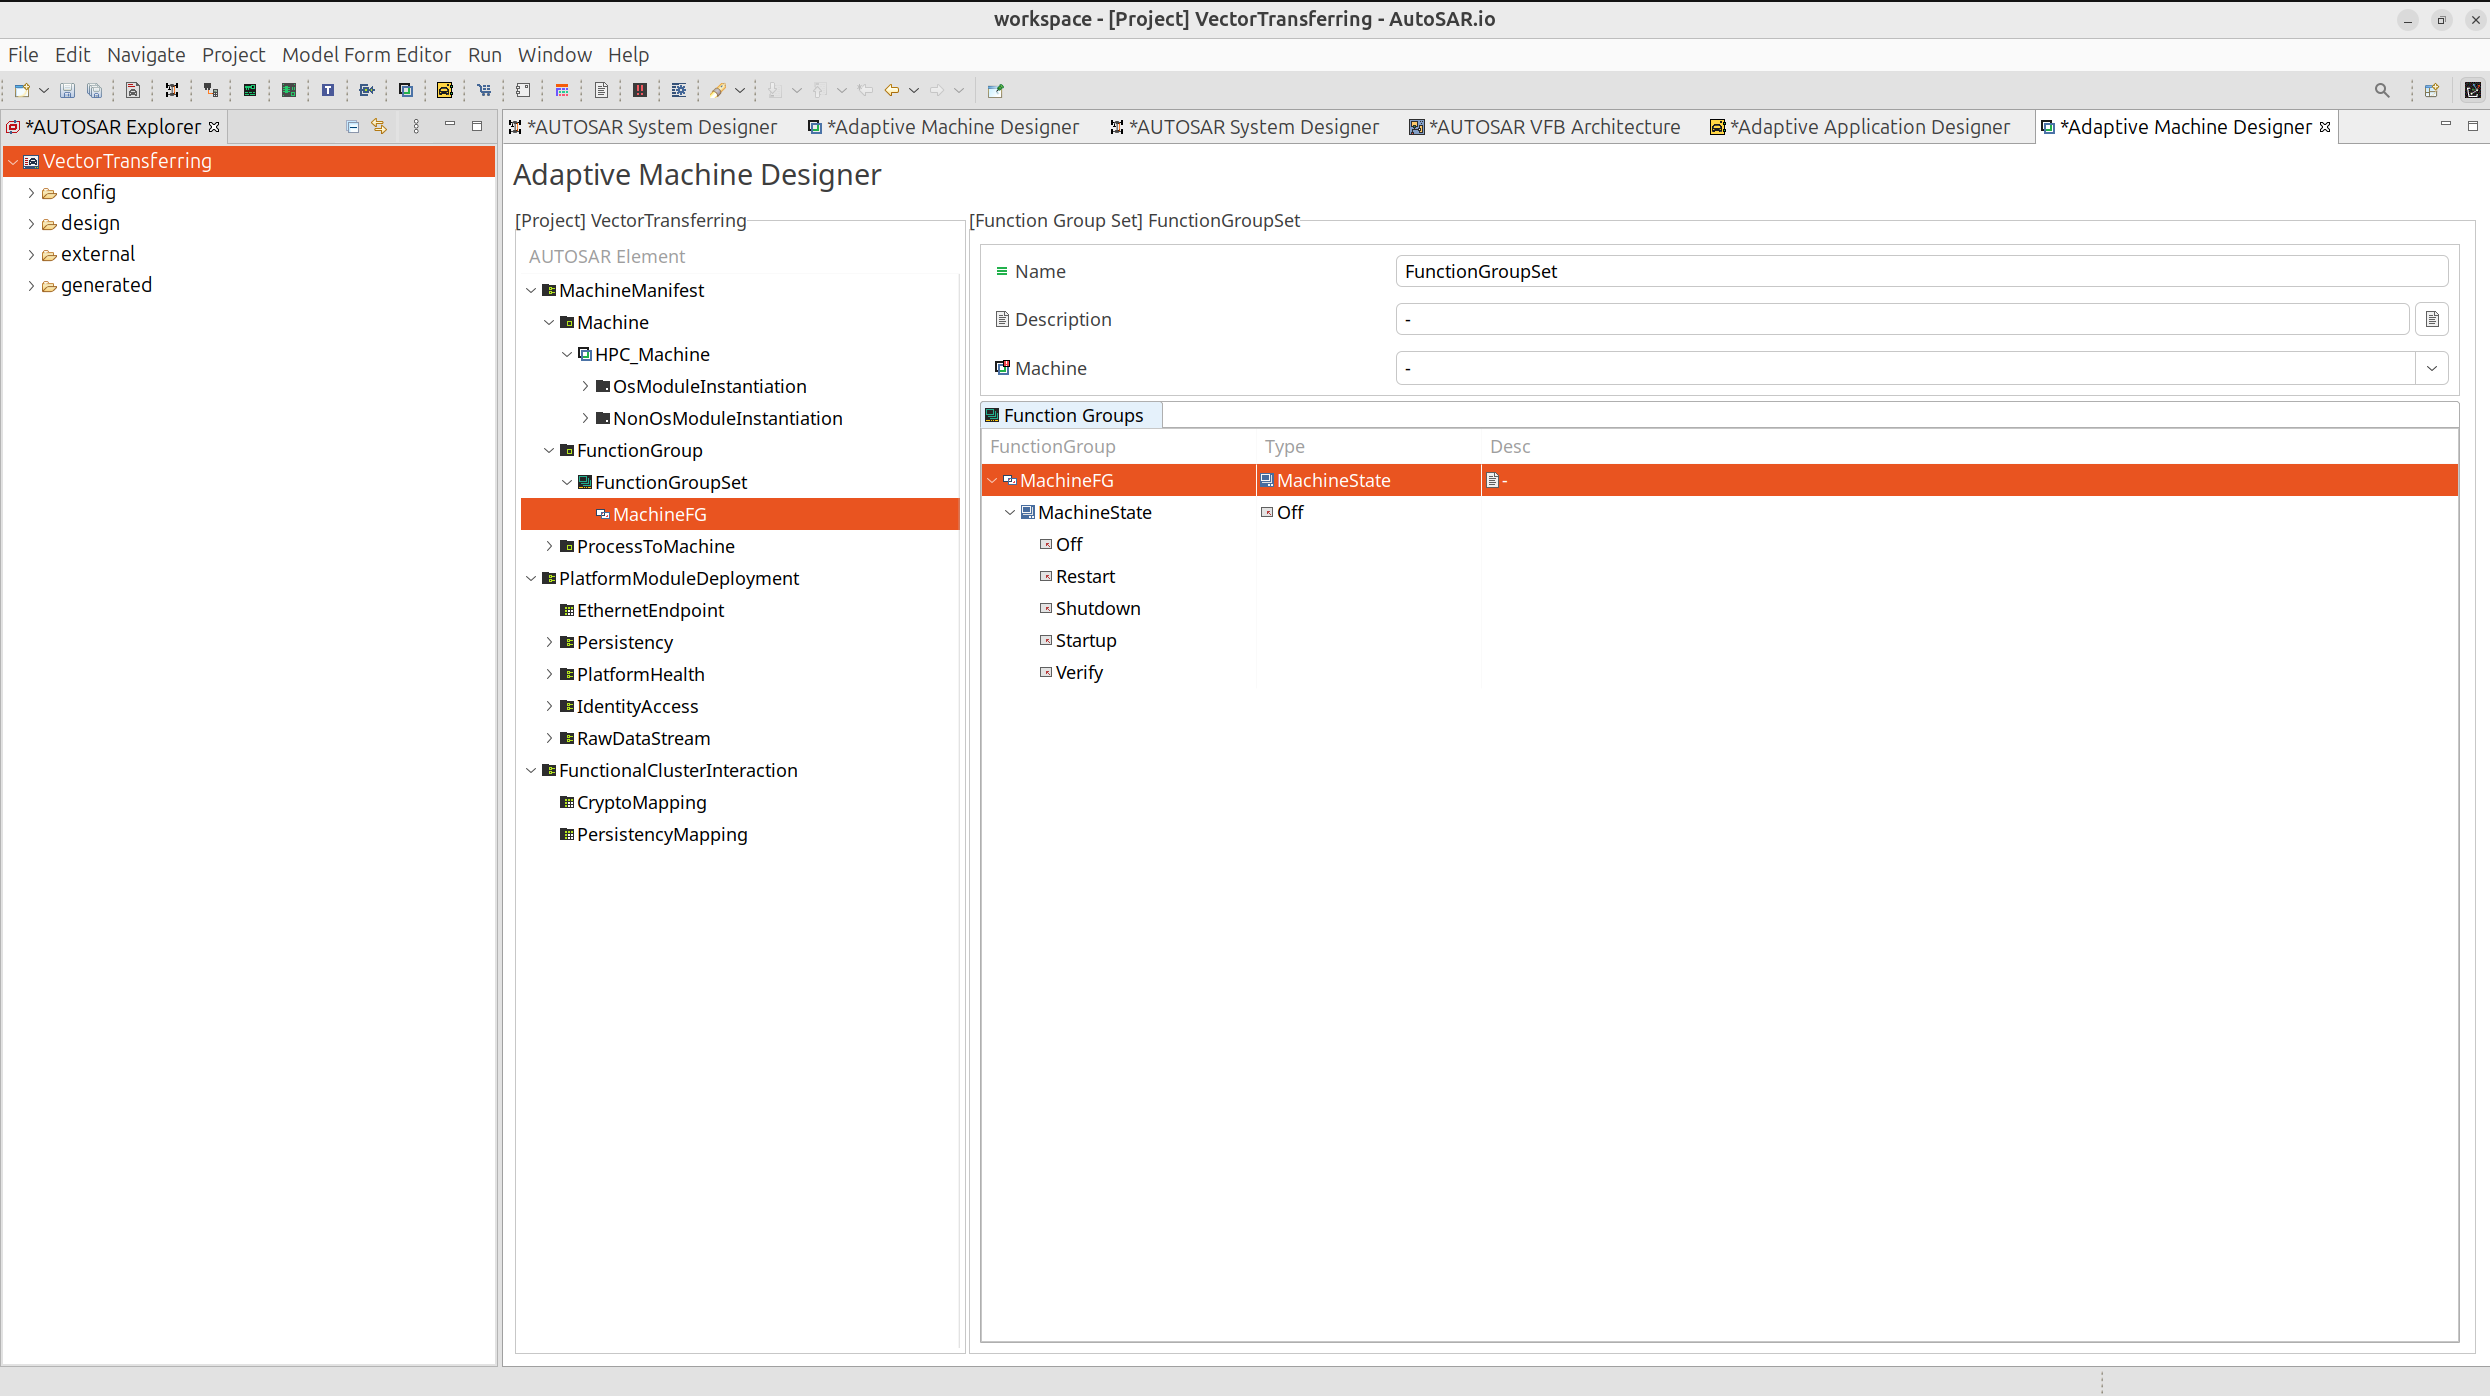
\includegraphics[width=0.75\textwidth]{Images/chap3/image_methodology/machineDesign/configMachineFG.png}
    \vspace{0.5cm}
    \caption{Machine Function Group States Configuration}
    \label{fig:machine_fg_config}
\end{figure}

The figure \ref{fig:machine_fg_config} presents the configuration of the machine function group for the HPC\_Machine in the Adaptive Machine Designer. A function group named MachineFG is defined with the MachineState type, which includes states such as Off, Startup, Verify, Restart, and Shutdown. This configuration governs how the machine progresses through its operational lifecycle, ensuring that platform services and applications are activated and controlled according to well defined system states during runtime execution.

% Final Machine Manifest
\begin{figure}[H]
    \centering
    
\includegraphics[width=0.75\textwidth]{Images/chap3/image_methodology/machineDesign/machineManifest.png}
    \vspace{0.5cm}
    \caption{Machine Manifest for Adaptive AUTOSAR Deployment}
    \label{fig:machine_manifest}
\end{figure}

The figure \ref{fig:machine_manifest} presents the Machine Manifest of the HPC\_Machine as defined in the Adaptive Machine Designer. This manifest consolidates all machine level configurations by referencing the previously defined Machine Design, including the SOME/IP Service Discovery endpoint with the multicast address 224.0.0.1 and port 30490, as well as the Ethernet connector bound to the eth0 interface. In addition, user defined connectors and inter process communication settings are integrated, forming a complete description of the communication capabilities of the target machine.

Furthermore, the manifest specifies essential execution and platform related properties such as trusted platform execution mode, default application timeout, and processor configuration. The processor section defines the available CPU resources and core assignment, while function group and process to machine mappings establish how applications are bound to machine states at runtime. By combining communication, execution, and lifecycle information into a single artifact, the Machine Manifest serves as the final deployment blueprint for Adaptive AUTOSAR applications.

% Configure Operating System platform module
\begin{figure}[H]
    \centering
    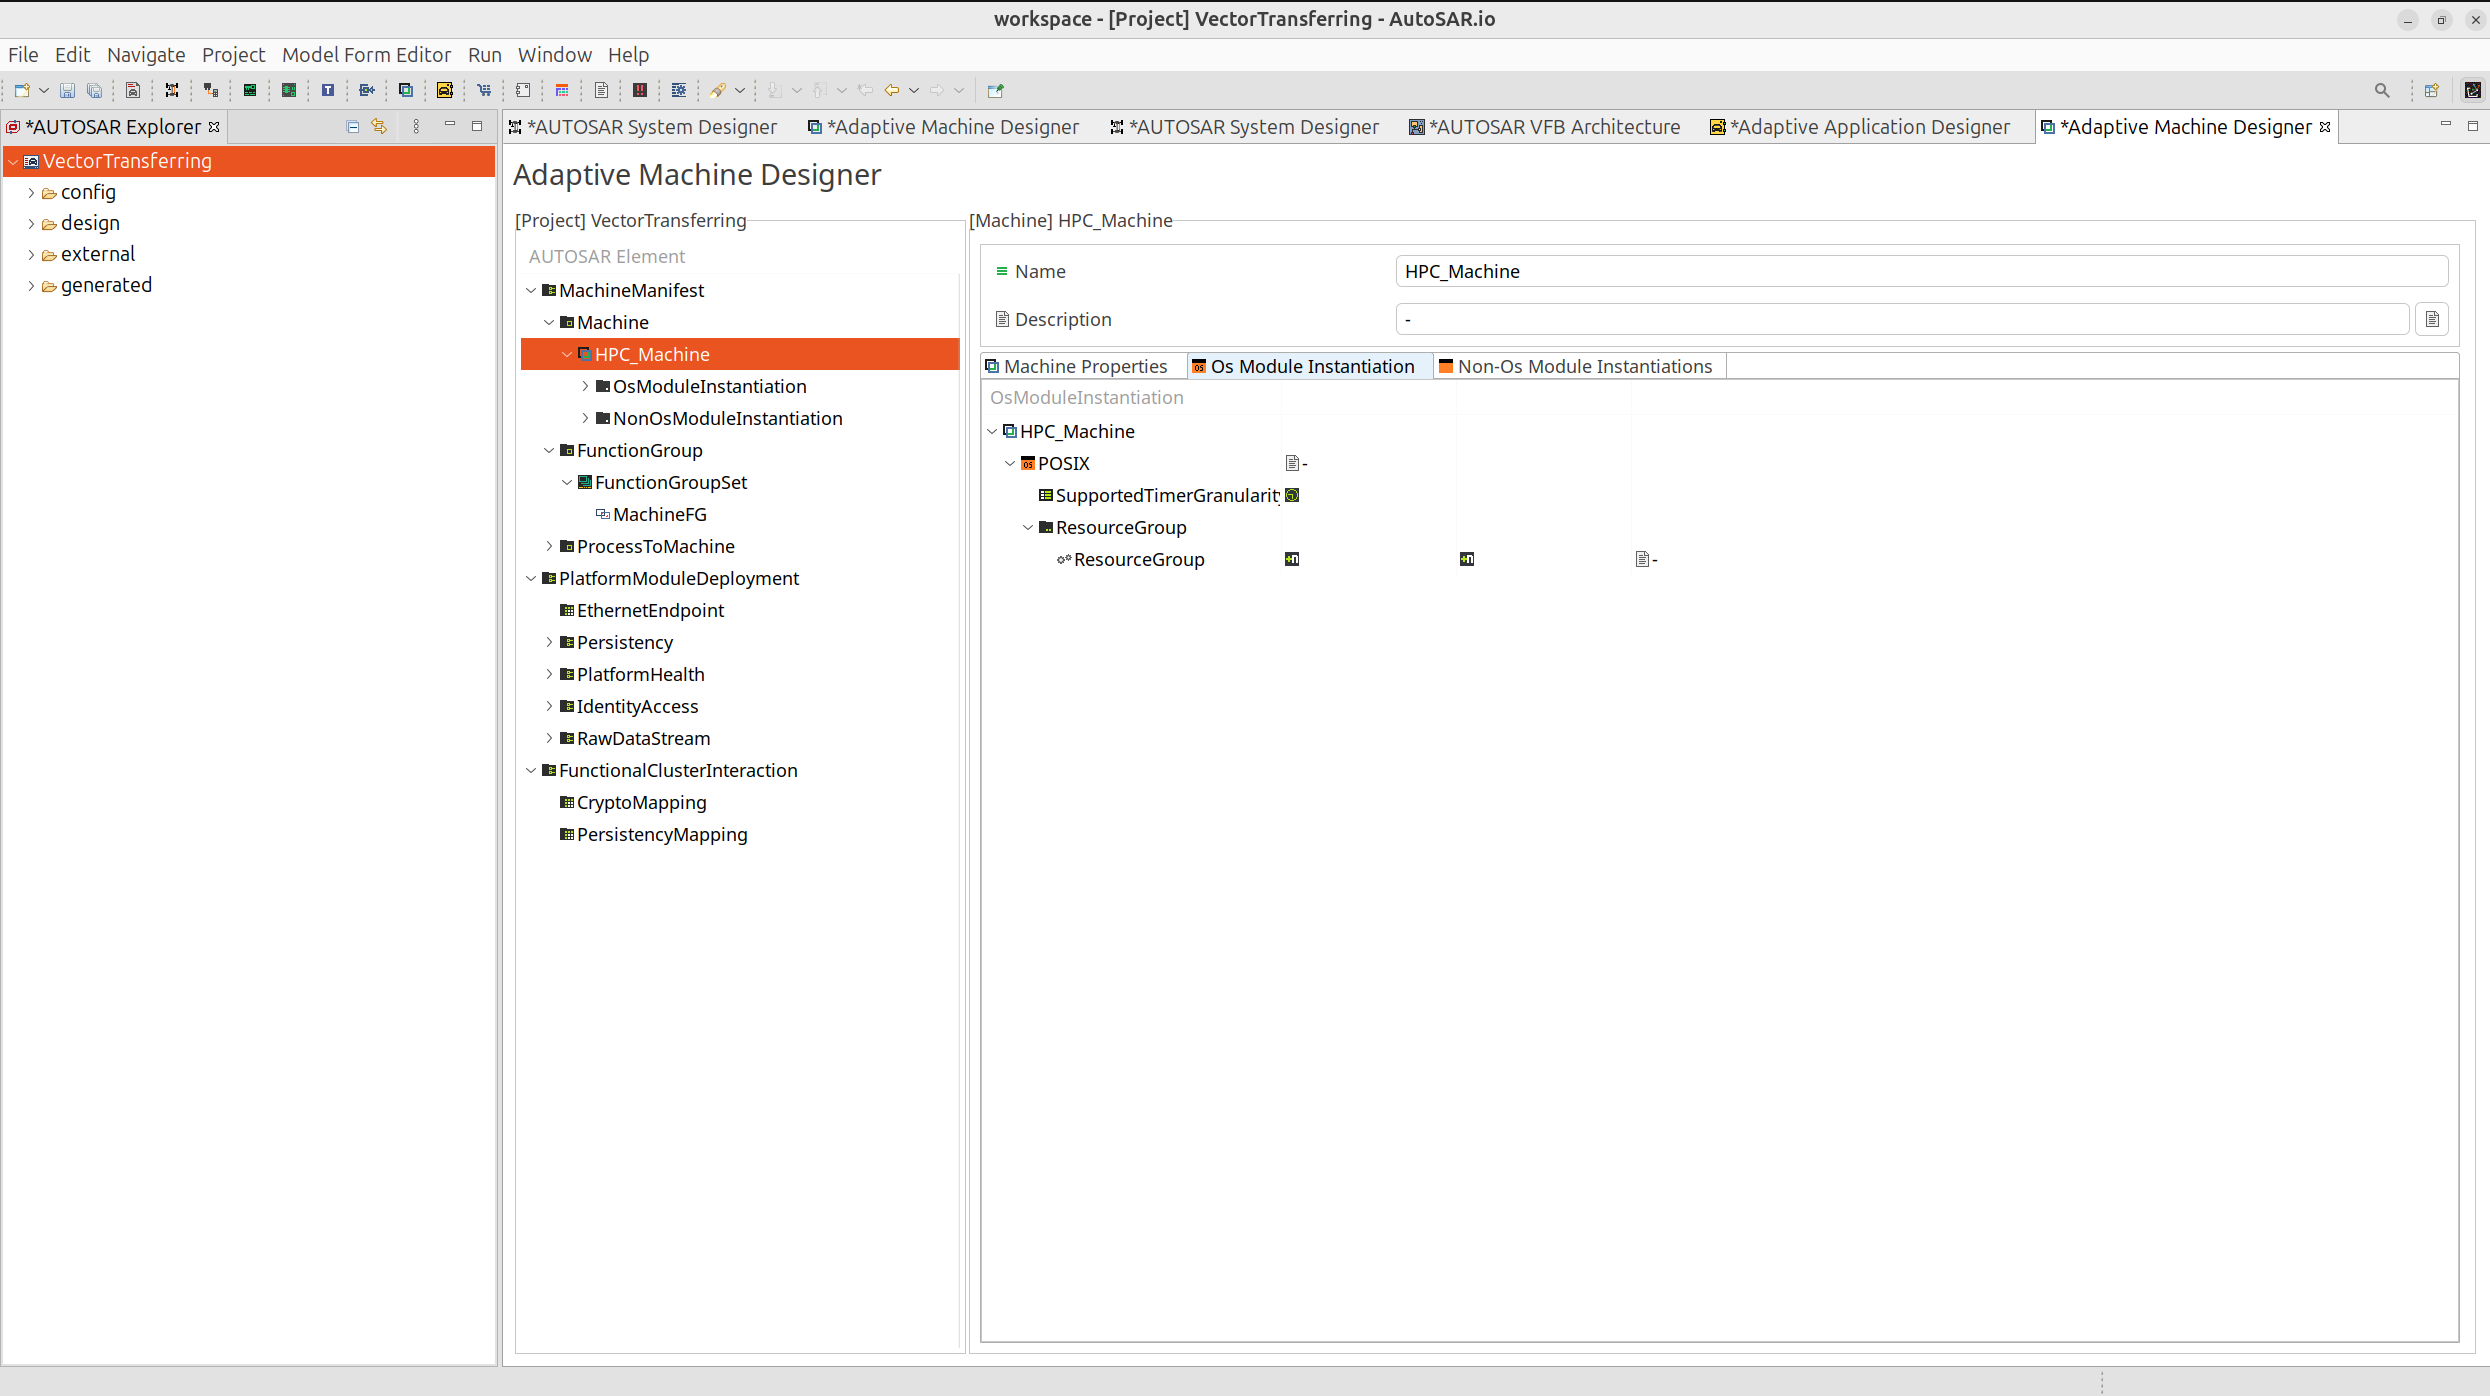
\includegraphics[width=0.75\textwidth]{Images/chap3/image_methodology/machineDesign/configOSModule.png}
    \vspace{0.5cm}
    \caption{Operating System Platform Module Configuration}
    \label{fig:machine_os_module}
\end{figure}

Figure~\ref{fig:machine_os_module} shows the operating system platform module configuration for the target machine named HPC\_Machine in the Adaptive Machine Designer. The POSIX based operating system module is instantiated to define the execution environment for Adaptive AUTOSAR applications, including supported timer granularity and resource group settings. This configuration establishes the fundamental runtime services required for process scheduling and resource management on the target machine.

% Configure non-OS platform modules
\begin{figure}[H]
    \centering
    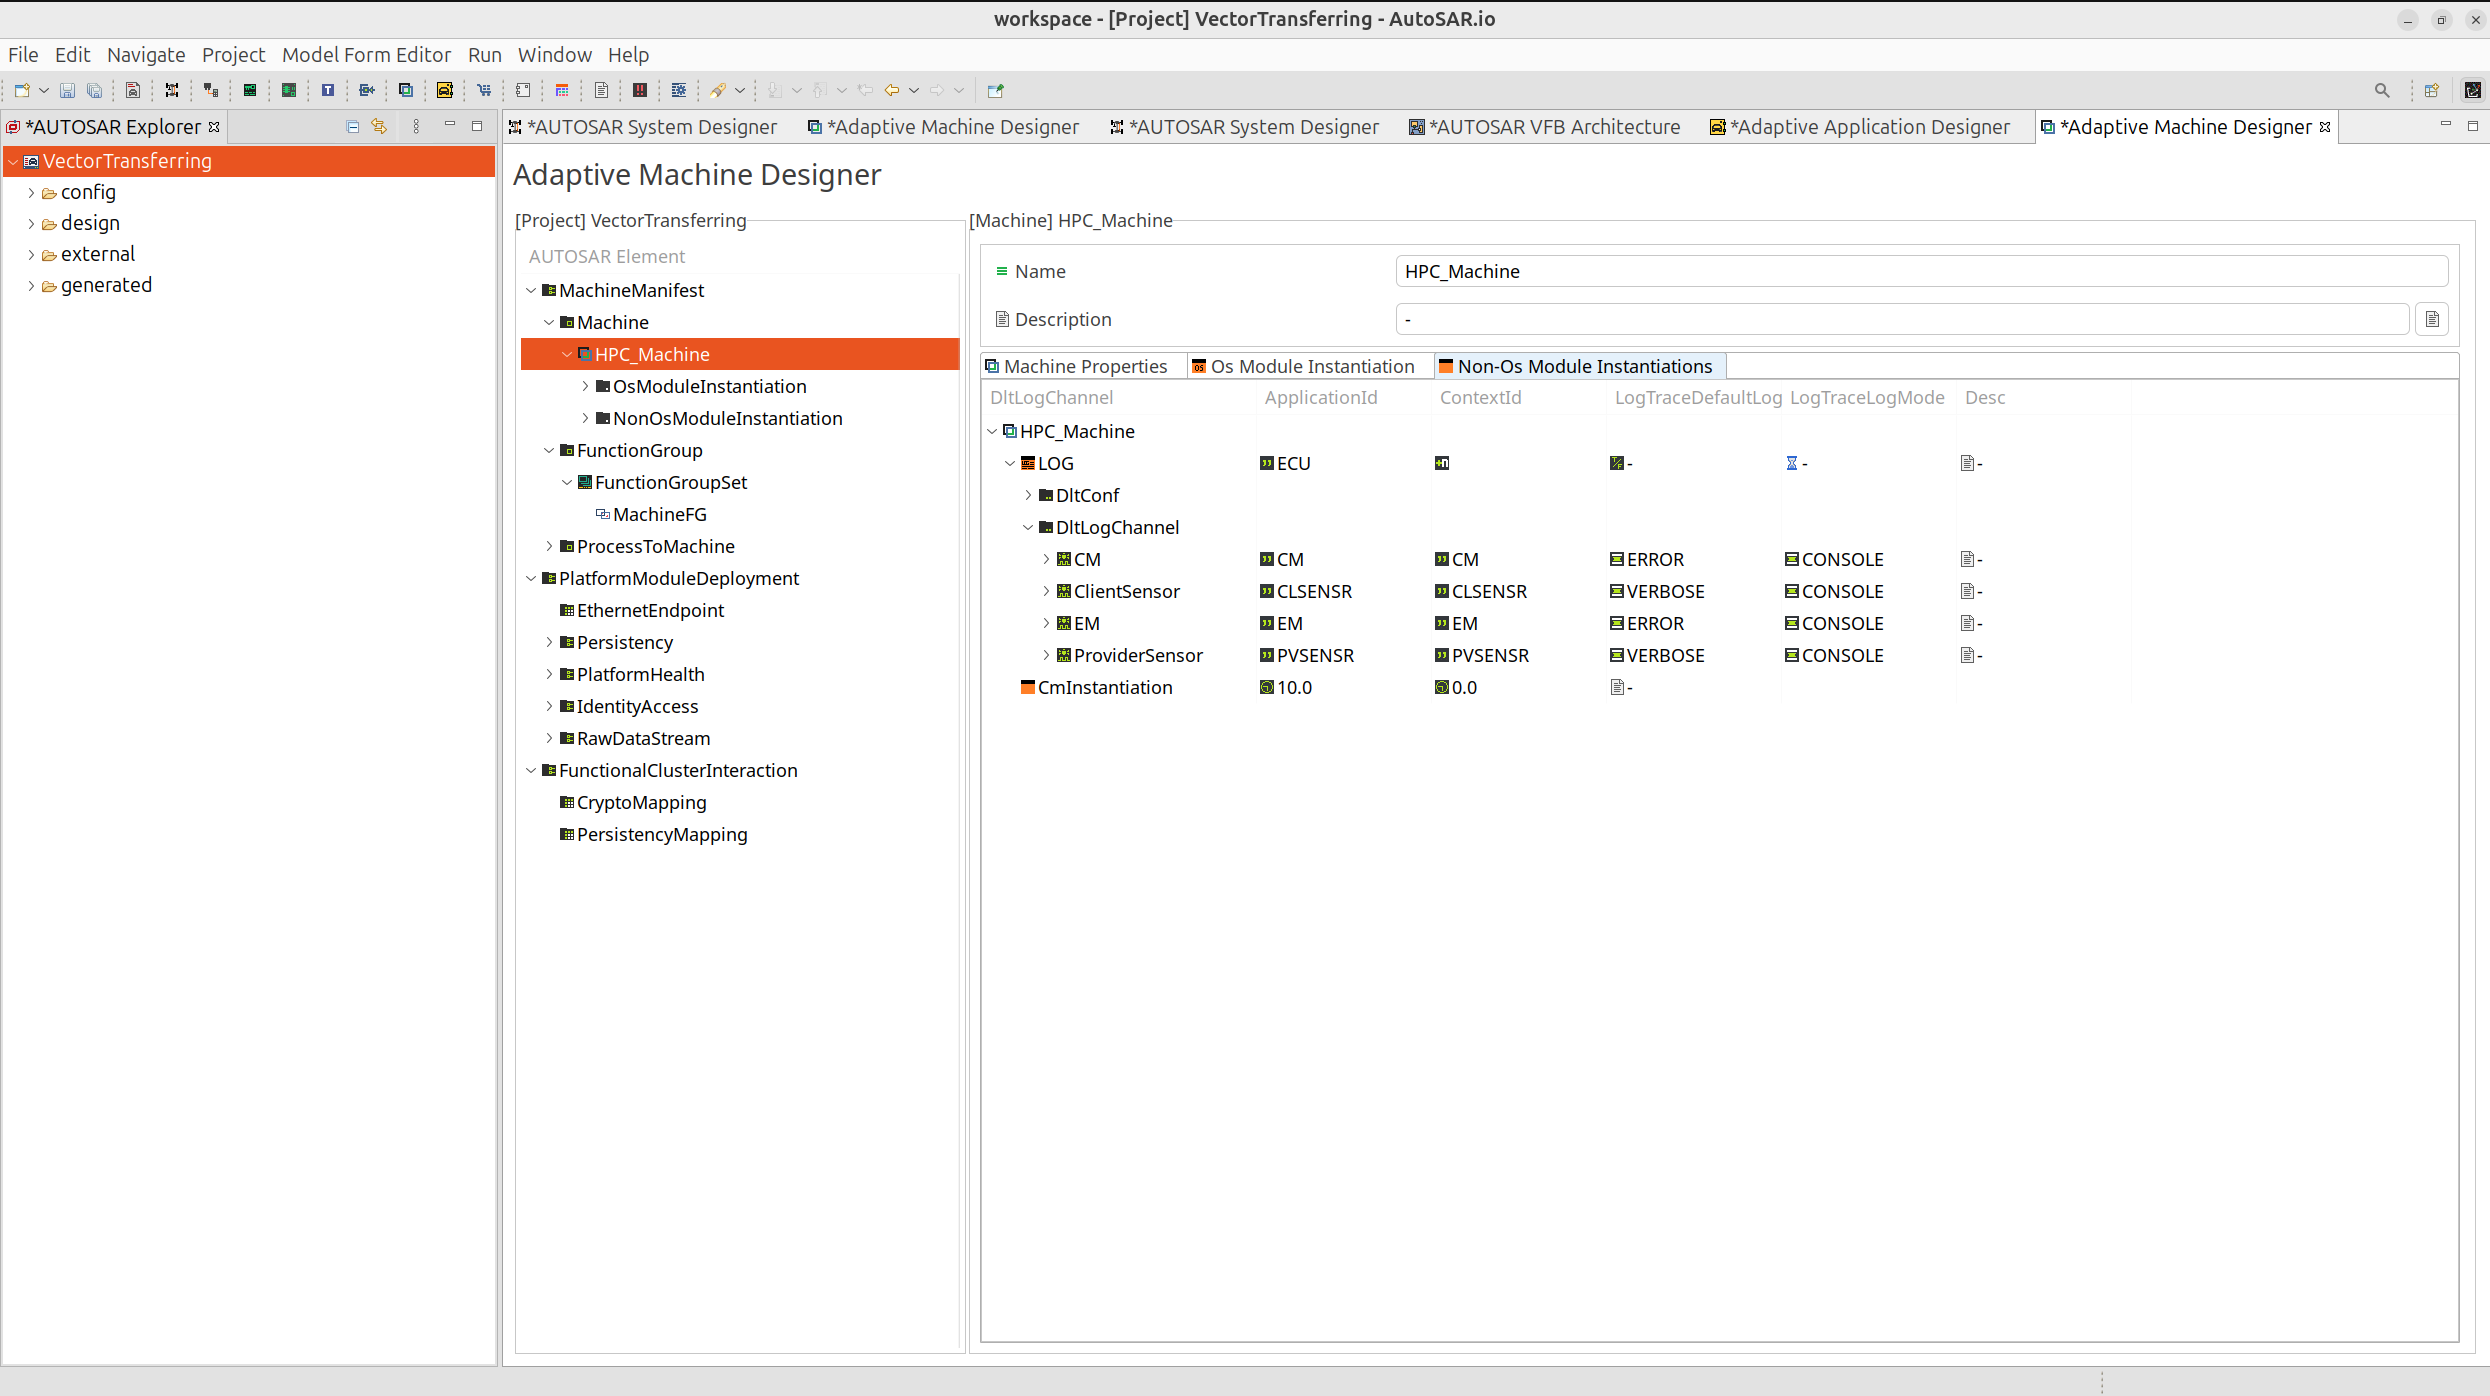
\includegraphics[width=0.75\textwidth]{Images/chap3/image_methodology/machineDesign/configNonOS.png}
    \vspace{0.5cm}
    \caption{Configuration of Non-OS Platform Modules}
    \label{fig:machine_non_os_module}
\end{figure}

Figure~\ref{fig:machine_non_os_module} presents the configuration of Diagnostic Log and Trace for the HPC\_Machine in the Adaptive Machine Designer. Several log channels are defined for different software entities, including ECU, ClientSensor, EM, and ProviderSensor, each mapped to a distinct ApplicationId and ContextId. Log levels such as ERROR and VERBOSE are specified, and the output is directed to the console, allowing developers to monitor application execution and diagnose runtime behavior.

In addition, the configuration highlights the role of CMInstantiation, which represents the Communication Management daemon responsible for inter process communication on the Adaptive Platform. This daemon enables different processes to exchange messages and supports the transport of diagnostic data between applications and platform services. By instantiating the communication manager at the machine level, the system ensures that logging, tracing, and service communication operate coherently across all running processes.

\subsubsection{Service Interface Design and Mapping}

% Define data types for service interfaces
\begin{figure}[H]
    \centering
    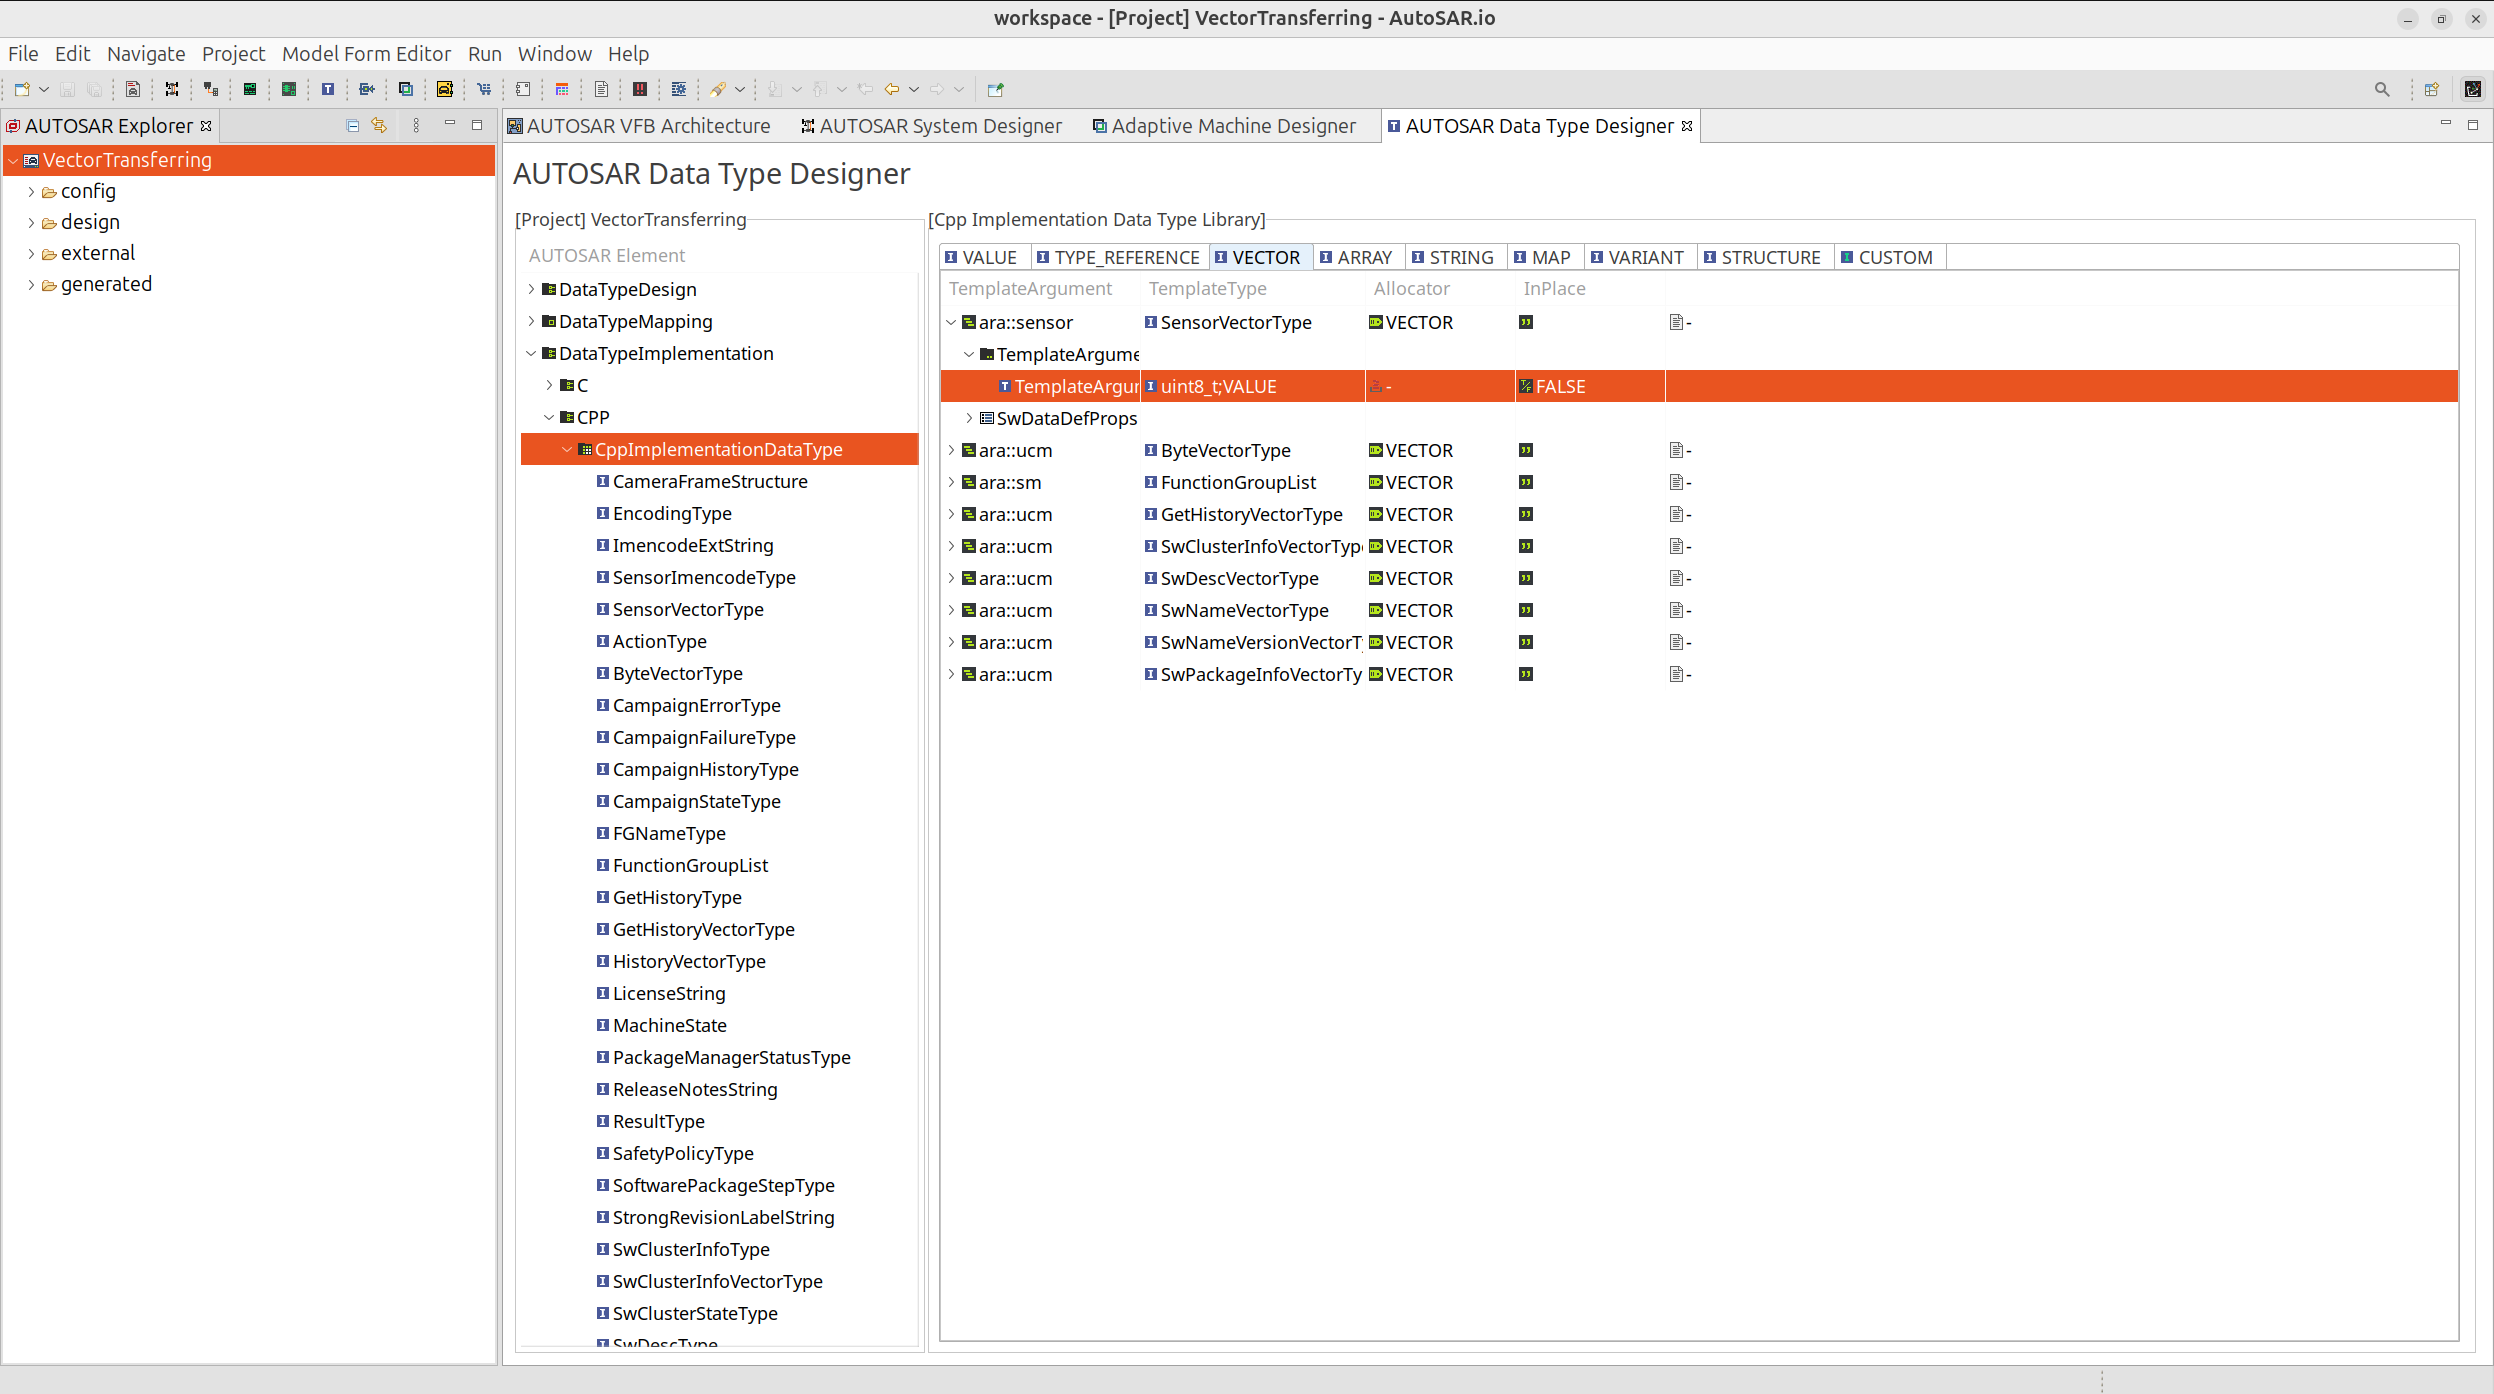
\includegraphics[width=0.75\textwidth]{Images/chap3/image_methodology/serviceInterfaceDesign/dataType.png}
    \vspace{0.5cm}
    \caption{Definition of Data Types for Service Interfaces}
    \label{fig:service_datatype}
\end{figure}

The figure~\ref{fig:service_datatype} shows the specification of C++ data types used to support service interfaces in the Adaptive AUTOSAR environment. Several vector based types are defined using template arguments, where primitive elements such as \texttt{uint8\_t} are combined to represent structured service data. These type definitions provide a clear and reusable foundation for data exchange between service providers and consumers, ensuring consistency and type safety during service oriented communication.

% Define service interface
\begin{figure}[H]
    \centering
    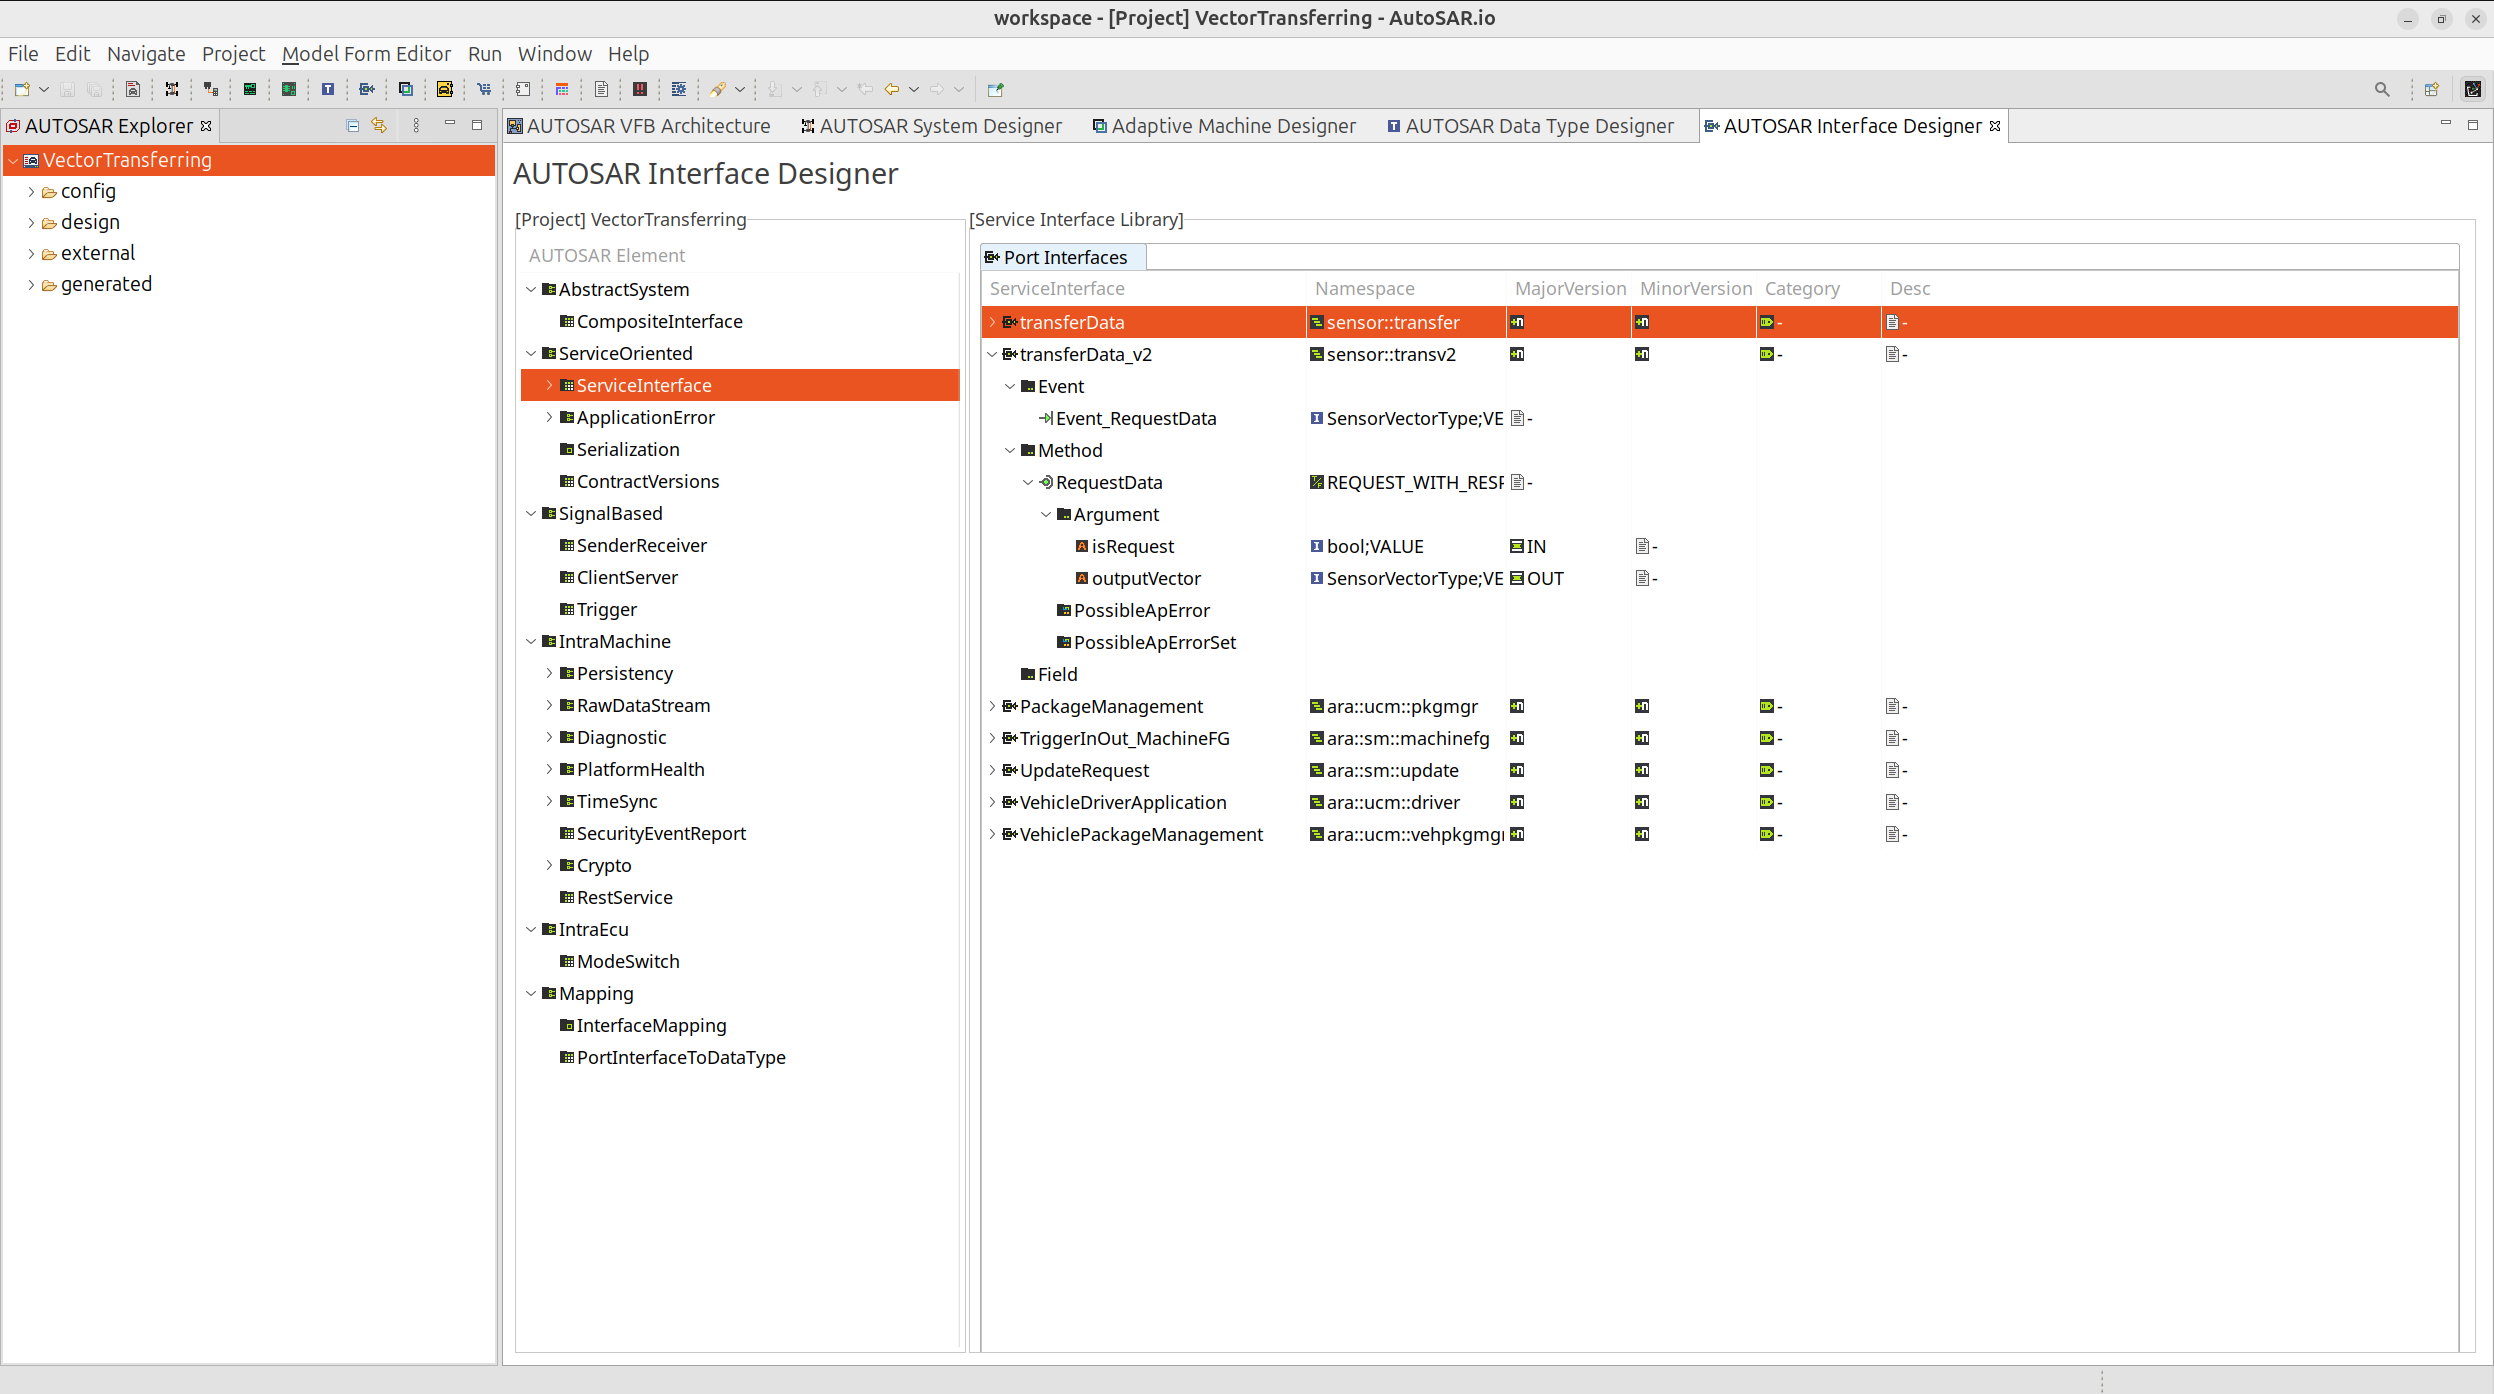
\includegraphics[width=0.75\textwidth]{Images/chap3/image_methodology/serviceInterfaceDesign/defineServiceInterface.png}
    \vspace{0.5cm}
    \caption{Service Interface Definition in Adaptive AUTOSAR}
    \label{fig:service_interface_definition}
\end{figure}

Figure~\ref{fig:service_interface_definition} illustrates the definition of a service oriented interface in the AUTOSAR Interface Designer. The service interface named \texttt{transferData\_v2} is specified within the \texttt{sensor::transv2} namespace and versioned to support interface evolution. It exposes both an event and a method, where the event enables asynchronous notification of data availability, while the method defines a request response interaction pattern for controlled data transmission between applications.

In addition, the interface description includes detailed method arguments and data flow directions. The \texttt{RequestData} method accepts an input parameter that influences the request behavior and produces an output vector based on the previously defined sensor data type. The event is associated with the same data representation (\texttt{Event\_RequestData}), allowing consumers to receive updates without explicitly issuing a request. Possible application errors are also declared to handle exceptional conditions during execution. As shown in Figure~\ref{fig:service_interface_definition}, this interface design supports both reactive and on demand communication between service providers and consumers in the Adaptive AUTOSAR system.


% Service deployment configuration
\begin{figure}[H]
    \centering
    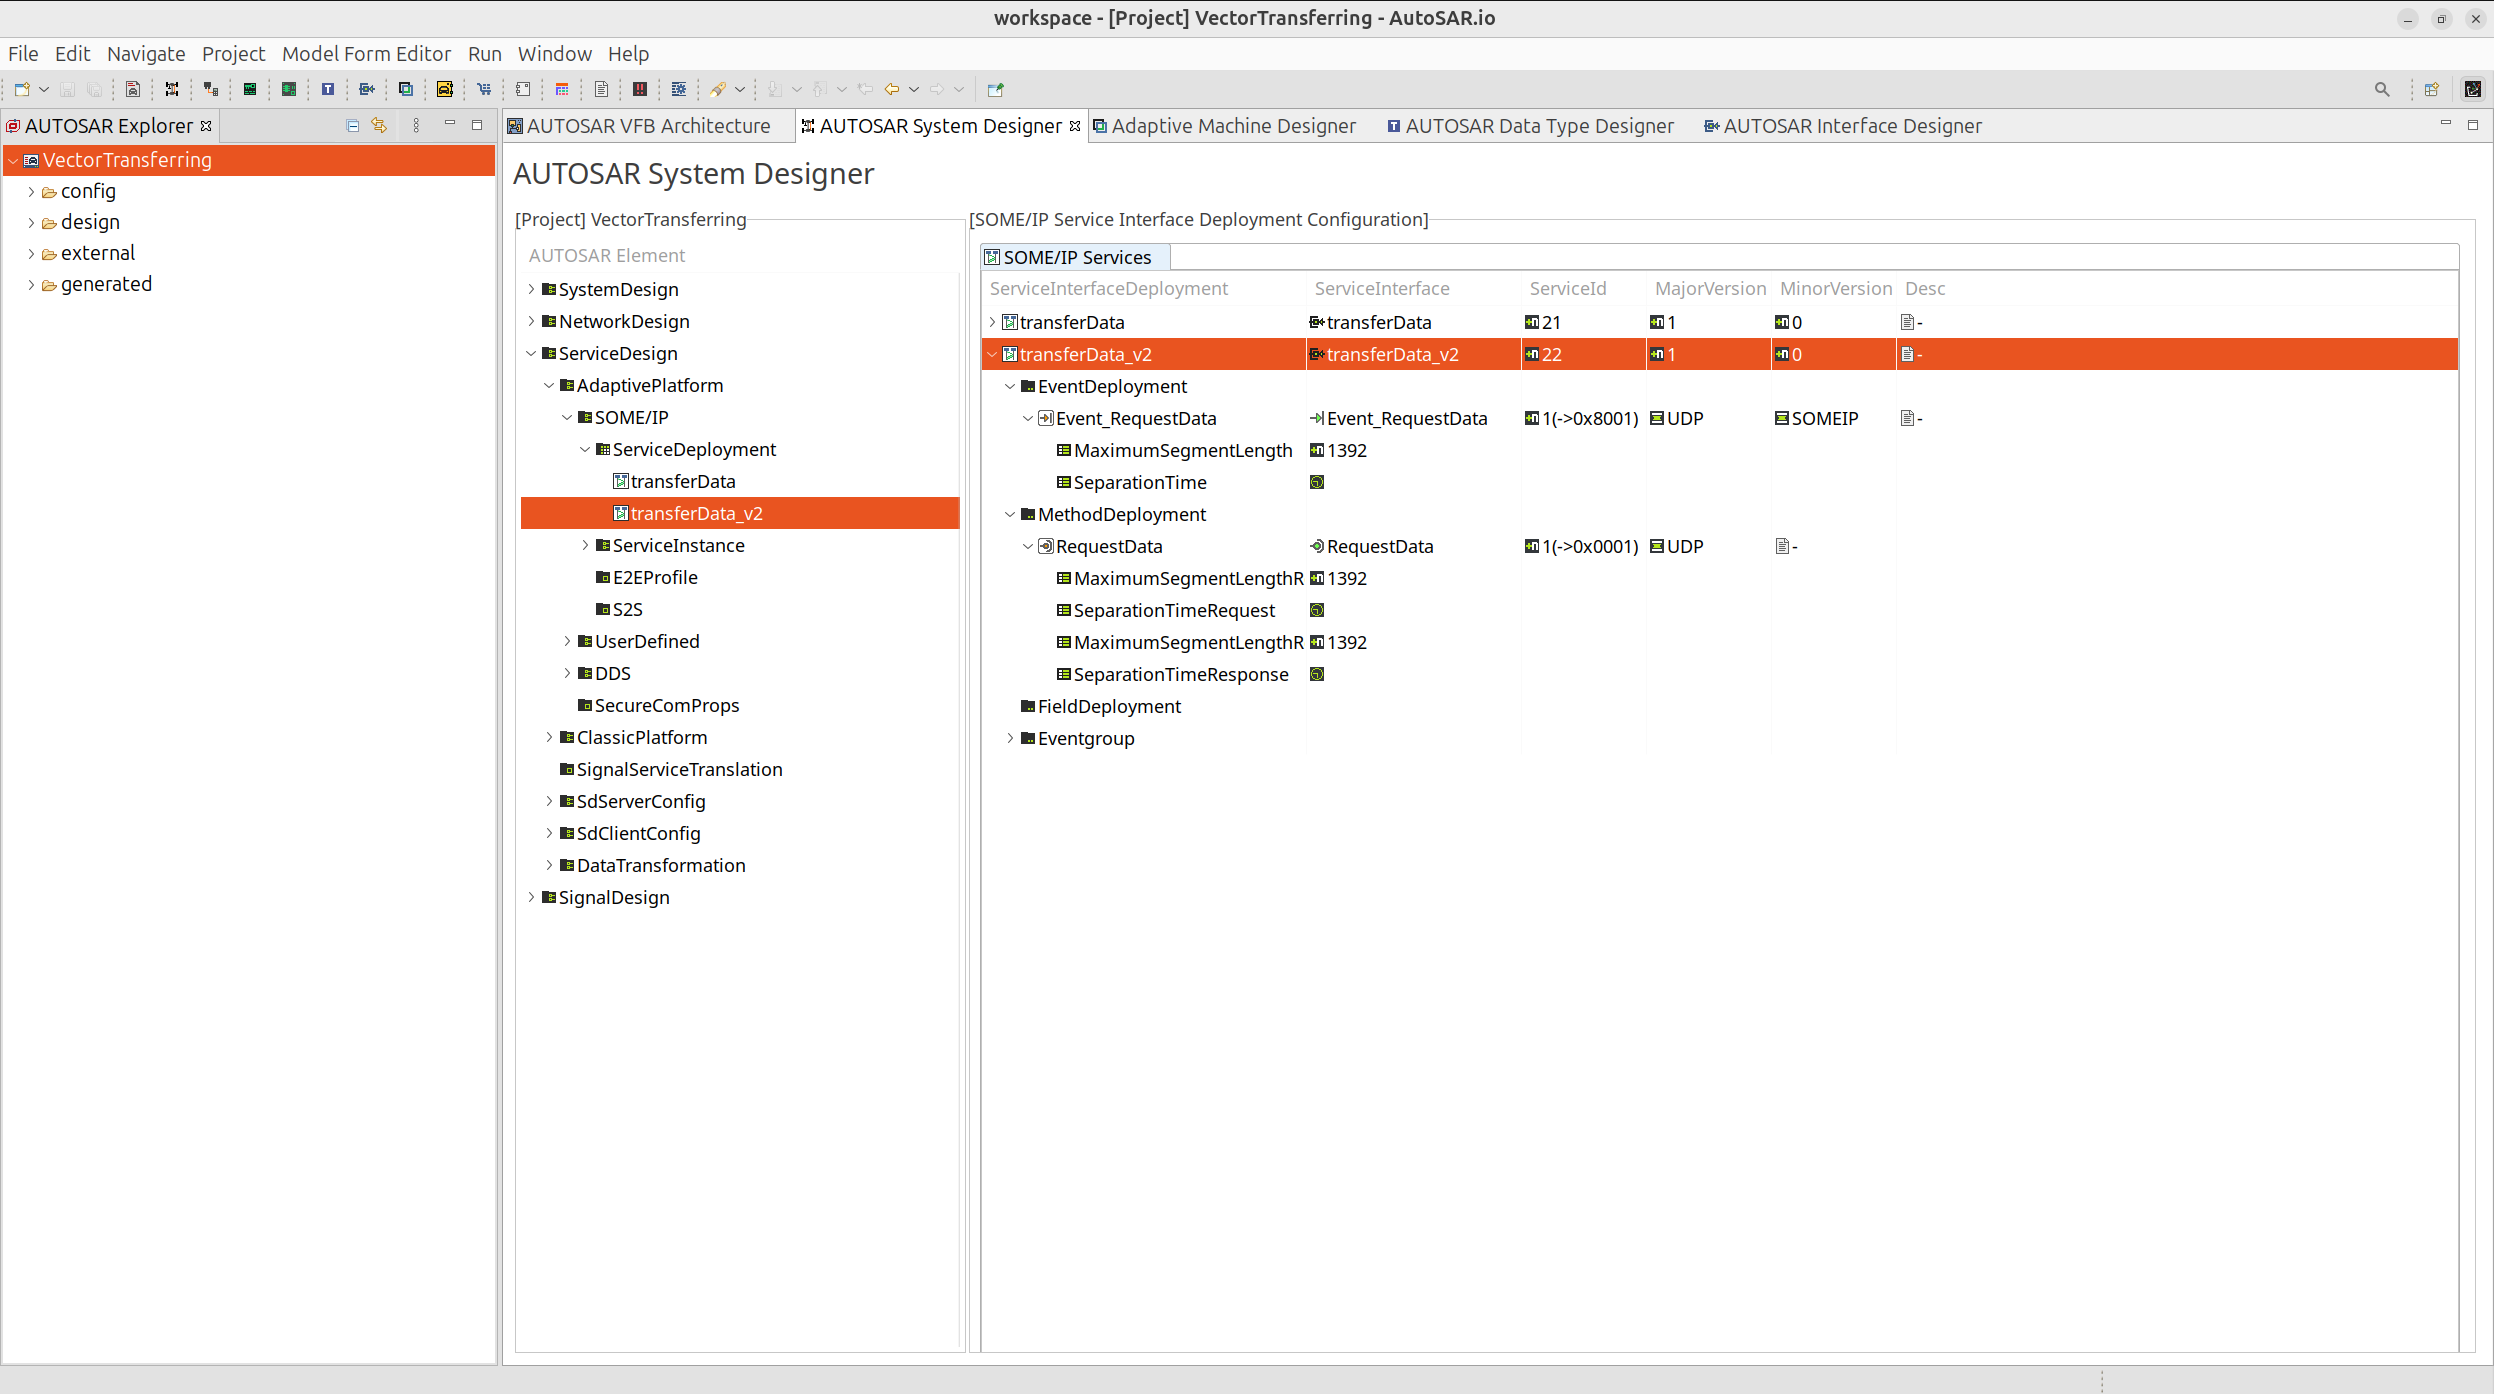
\includegraphics[width=0.75\textwidth]{Images/chap3/image_methodology/serviceInterfaceDesign/serviceDeployment.png}
    \vspace{0.5cm}
    \caption{Service Deployment Configuration}
    \label{fig:service_deployment}
\end{figure}

Figure~\ref{fig:service_deployment} illustrates the SOME/IP service deployment configuration for the \texttt{transferData\_v2} interface within the AUTOSAR System Designer. In this project, the service is explicitly deployed over SOME/IP with transport protocol (SOME/IP-TP) to support the transmission of large data payloads, such as image frames, between the ProviderSensor and ClientSensor applications.

The service is assigned a unique service identifier and version number and includes both event-based and method-based communication. The event \texttt{Event\_RequestData} is configured to use UDP transport together with a specified \texttt{MaximumSegmentLength}. This parameter plays a critical role in enabling SOME/IP-TP, as it informs the Adaptive AUTOSAR middleware that the transmitted data may exceed the maximum payload size of a single UDP packet and therefore must be segmented and reassembled at the receiver side.

Without configuring the \texttt{MaximumSegmentLength}, the communication would default to standard SOME/IP over UDP, which is suitable only for small messages and is not appropriate for transmitting image data. By explicitly defining this parameter, the deployment ensures that image payloads generated by the ProviderSensor are correctly fragmented, transmitted, and reassembled by the ClientSensor.

In addition to the event deployment, the \texttt{RequestData} method deployment specifies request and response timing parameters, supporting controlled client–server interaction when on-demand data transfer is required. Together, these configurations ensure that the \texttt{transferData\_v2} service can be reliably discovered via Service Discovery and can support both event-driven and request-based communication over SOME/IP-TP during runtime execution.


% Service instance provider configuration
\begin{figure}[H]
    \centering
    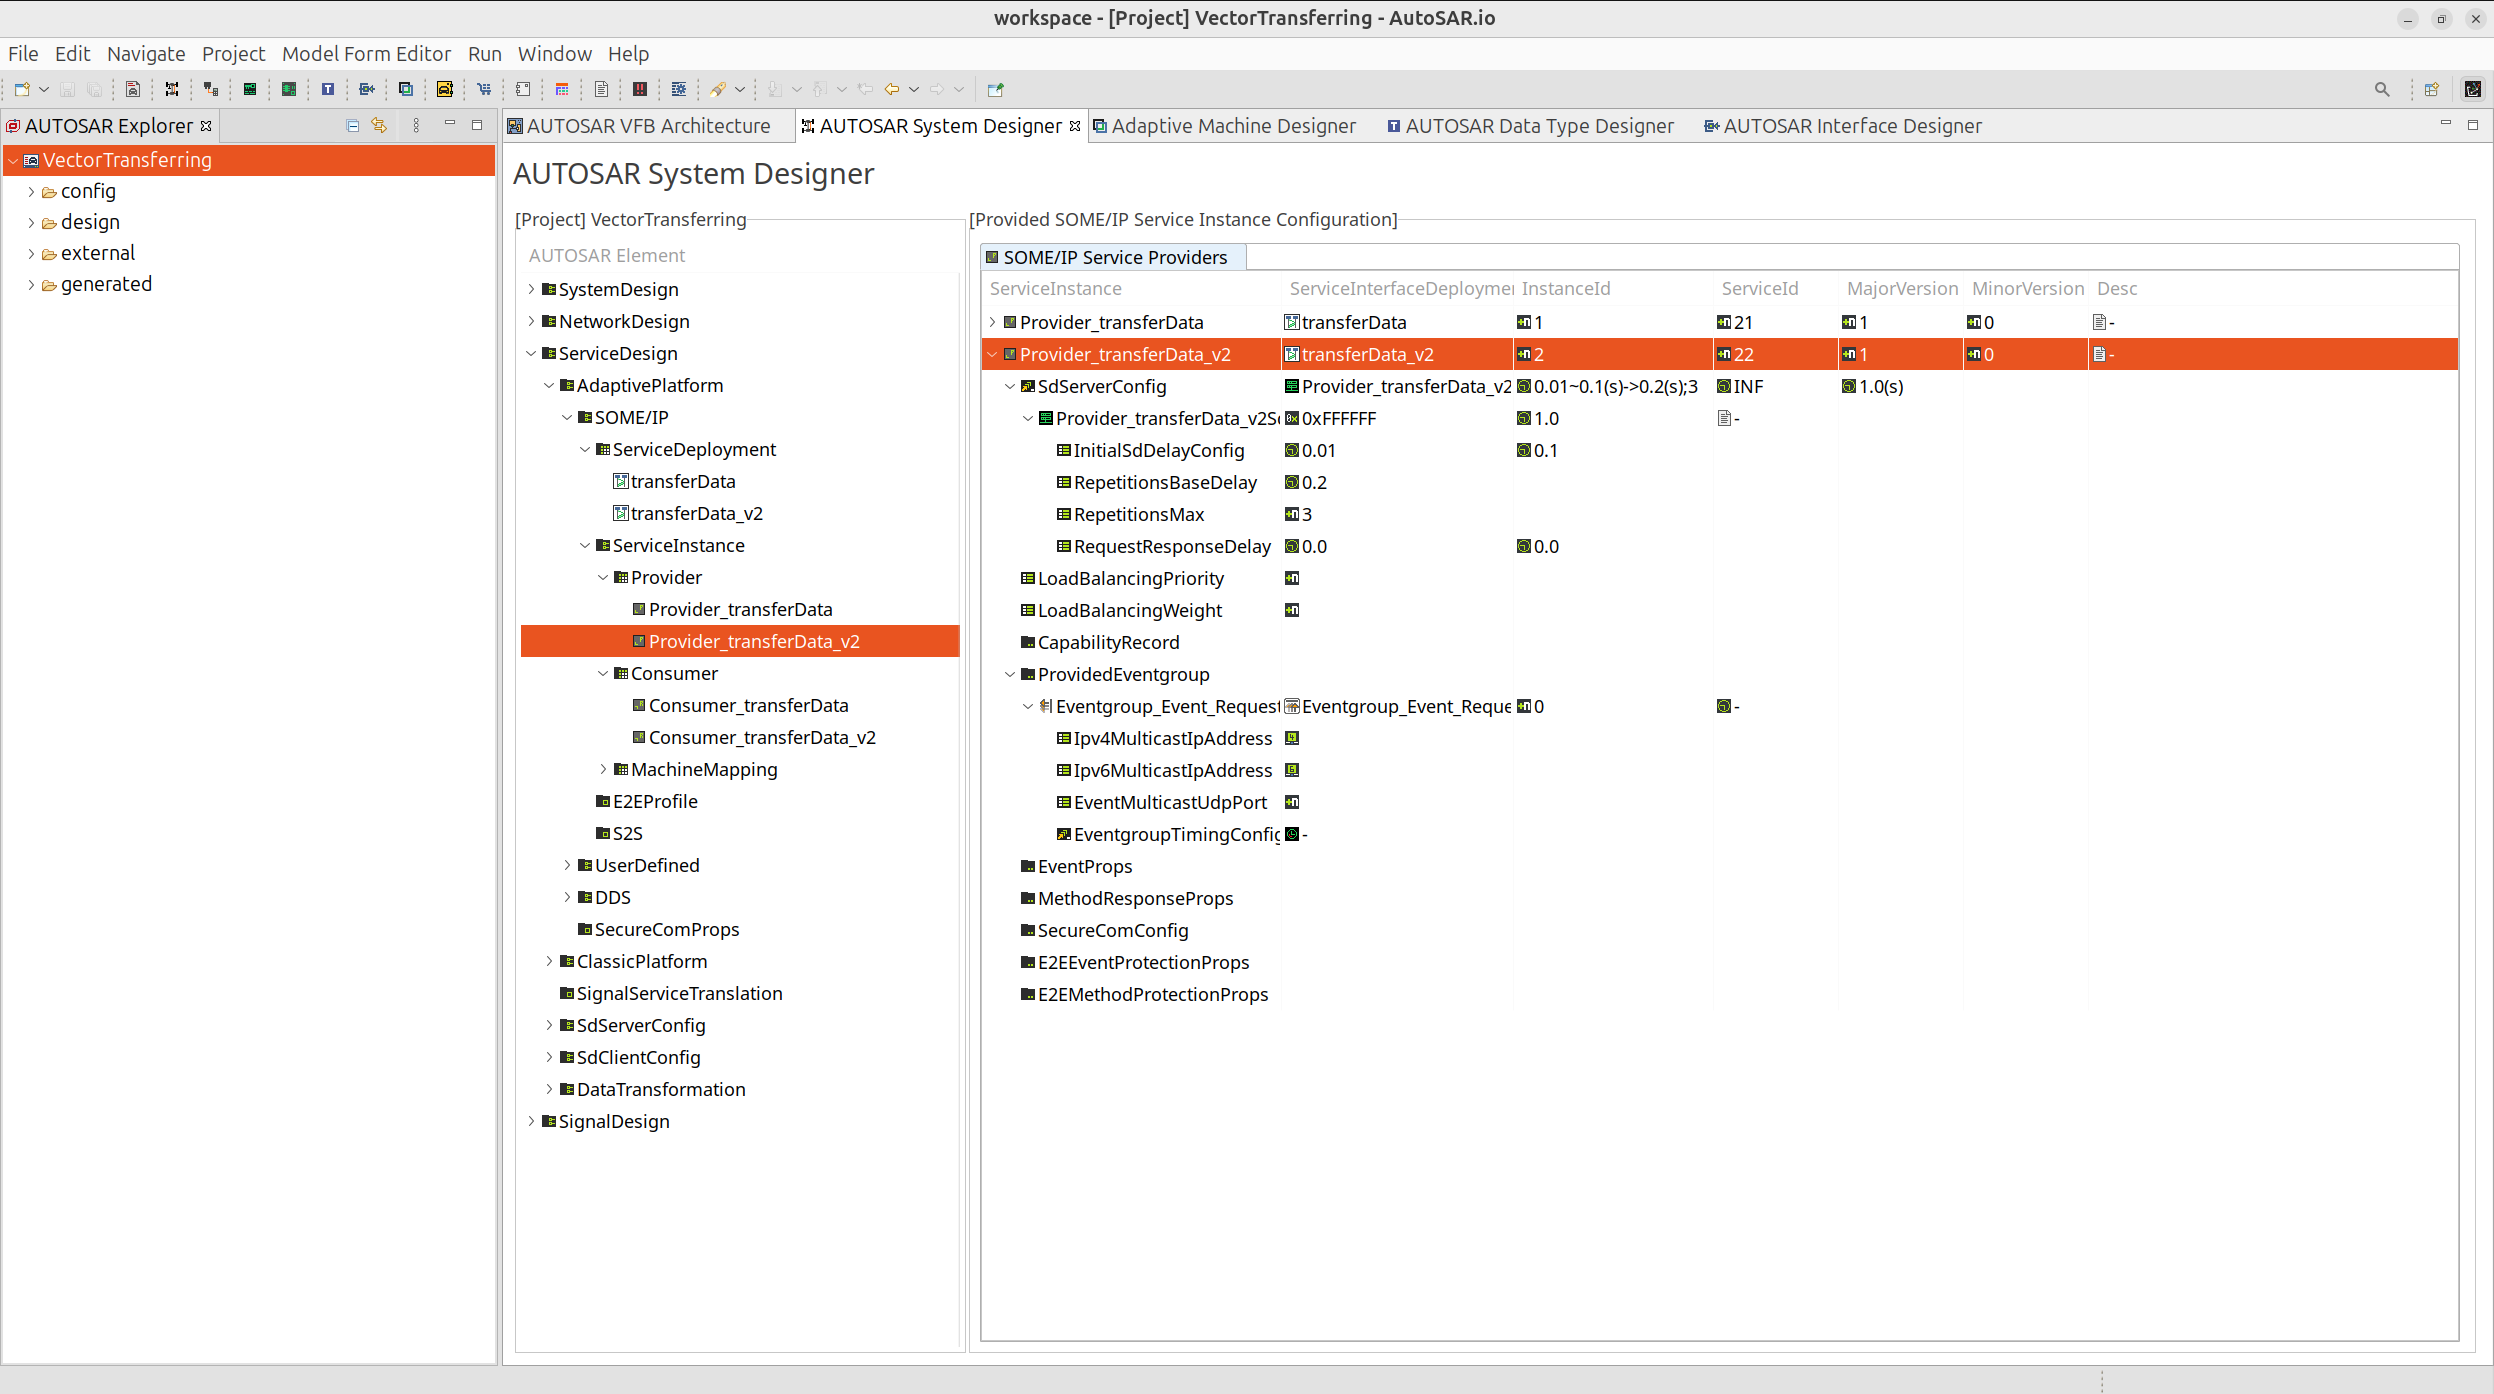
\includegraphics[width=0.75\textwidth]{Images/chap3/image_methodology/serviceInterfaceDesign/serviceInstance_Provider.png}
    \vspace{0.5cm}
    \caption{Service Instance Configuration for Provider}
    \label{fig:service_instance_provider}
\end{figure}

Figure~\ref{fig:service_instance_provider} illustrates the configuration of the SOME/IP service provider for the \texttt{transferData\_v2} interface. The provider instance is bound to a specific service and instance identifier with a defined major and minor version, ensuring compatibility with consuming applications. Server side parameters such as initial service offer delay, repetition base delay, and maximum repetitions are configured to control service availability announcements via Service Discovery. In addition, the provider defines event group settings for data notifications, together with timing and response related properties, which enable reliable dissemination of event based data to subscribed consumers during runtime.

% Service instance consumer configuration
\begin{figure}[H]
    \centering
    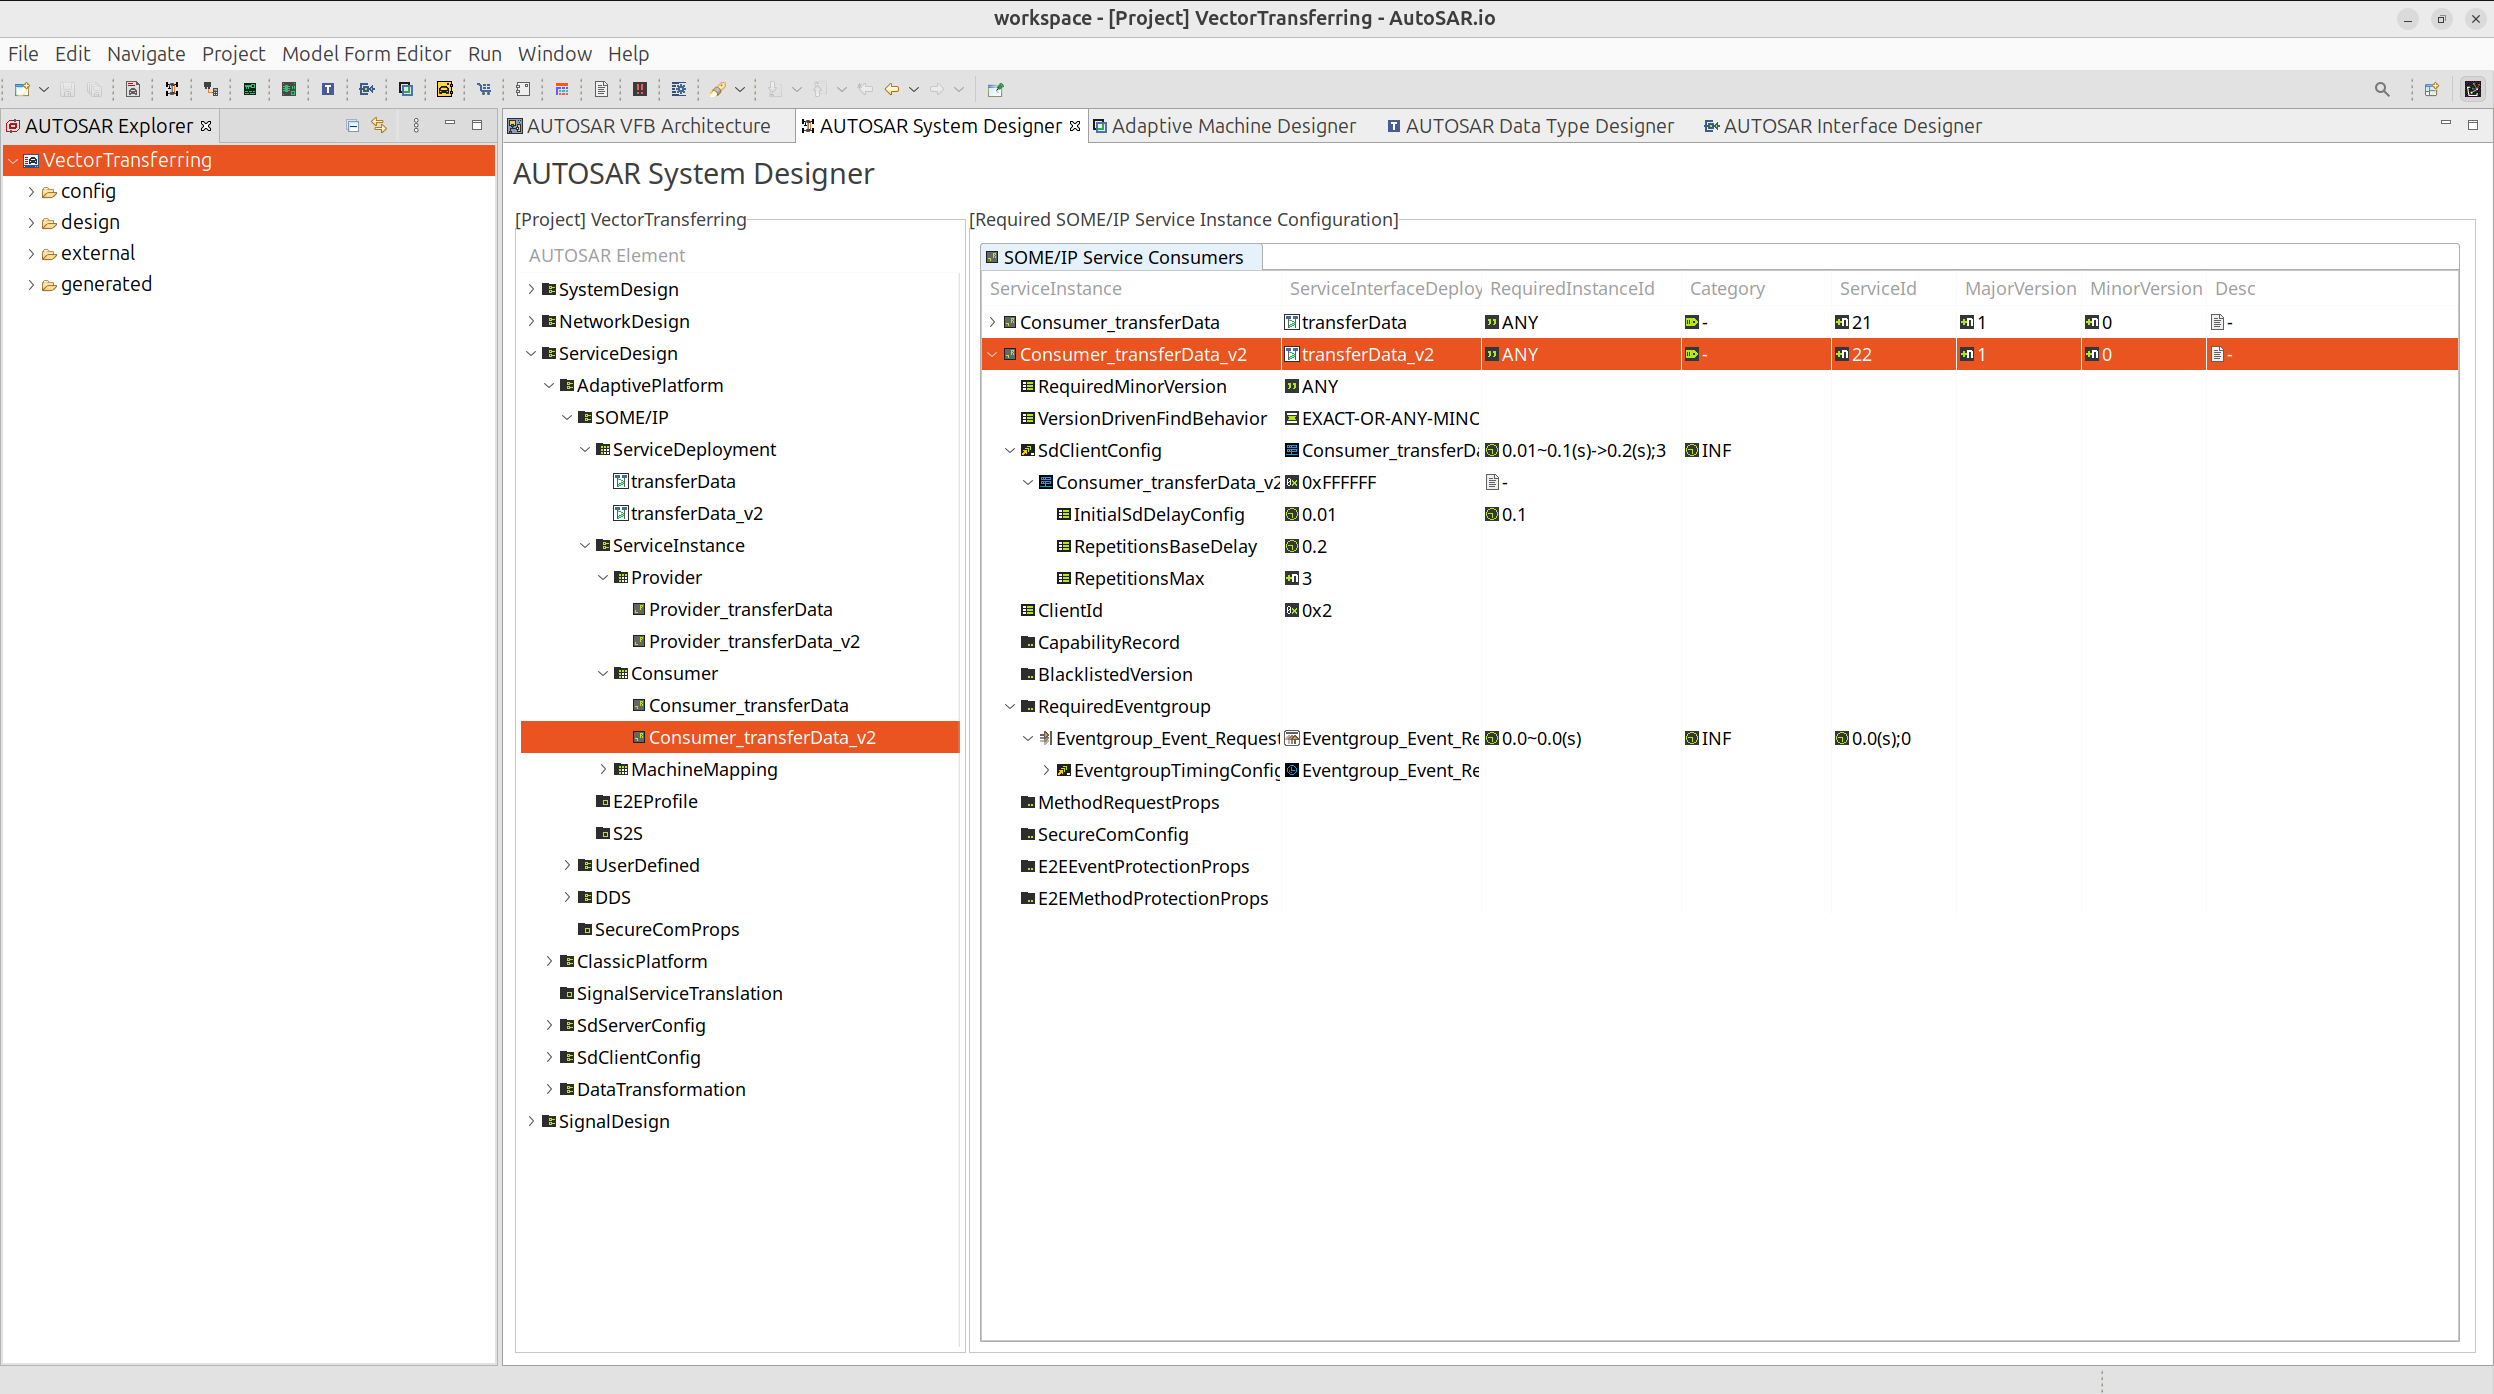
\includegraphics[width=0.75\textwidth]{Images/chap3/image_methodology/serviceInterfaceDesign/serviceInstance_Consumer.png}
    \vspace{0.5cm}
    \caption{Service Instance Configuration for Consumer}
    \label{fig:service_instance_consumer}
\end{figure}

Figure~\ref{fig:service_instance_consumer} presents the configuration of the corresponding SOME/IP service consumer acting as a subscriber to the \texttt{transferData\_v2} service. The consumer specifies flexible version requirements and discovery behavior, allowing it to bind to compatible provider instances at runtime. Client side parameters such as initial request delay, repetition strategy, and event group subscription settings determine how the consumer discovers the service and receives event notifications. Through this configuration, the consumer can dynamically subscribe to published data while maintaining controlled request and subscription behavior within the Adaptive AUTOSAR communication framework.

% Mapping service to machine network endpoint
\begin{figure}[H]
    \centering
    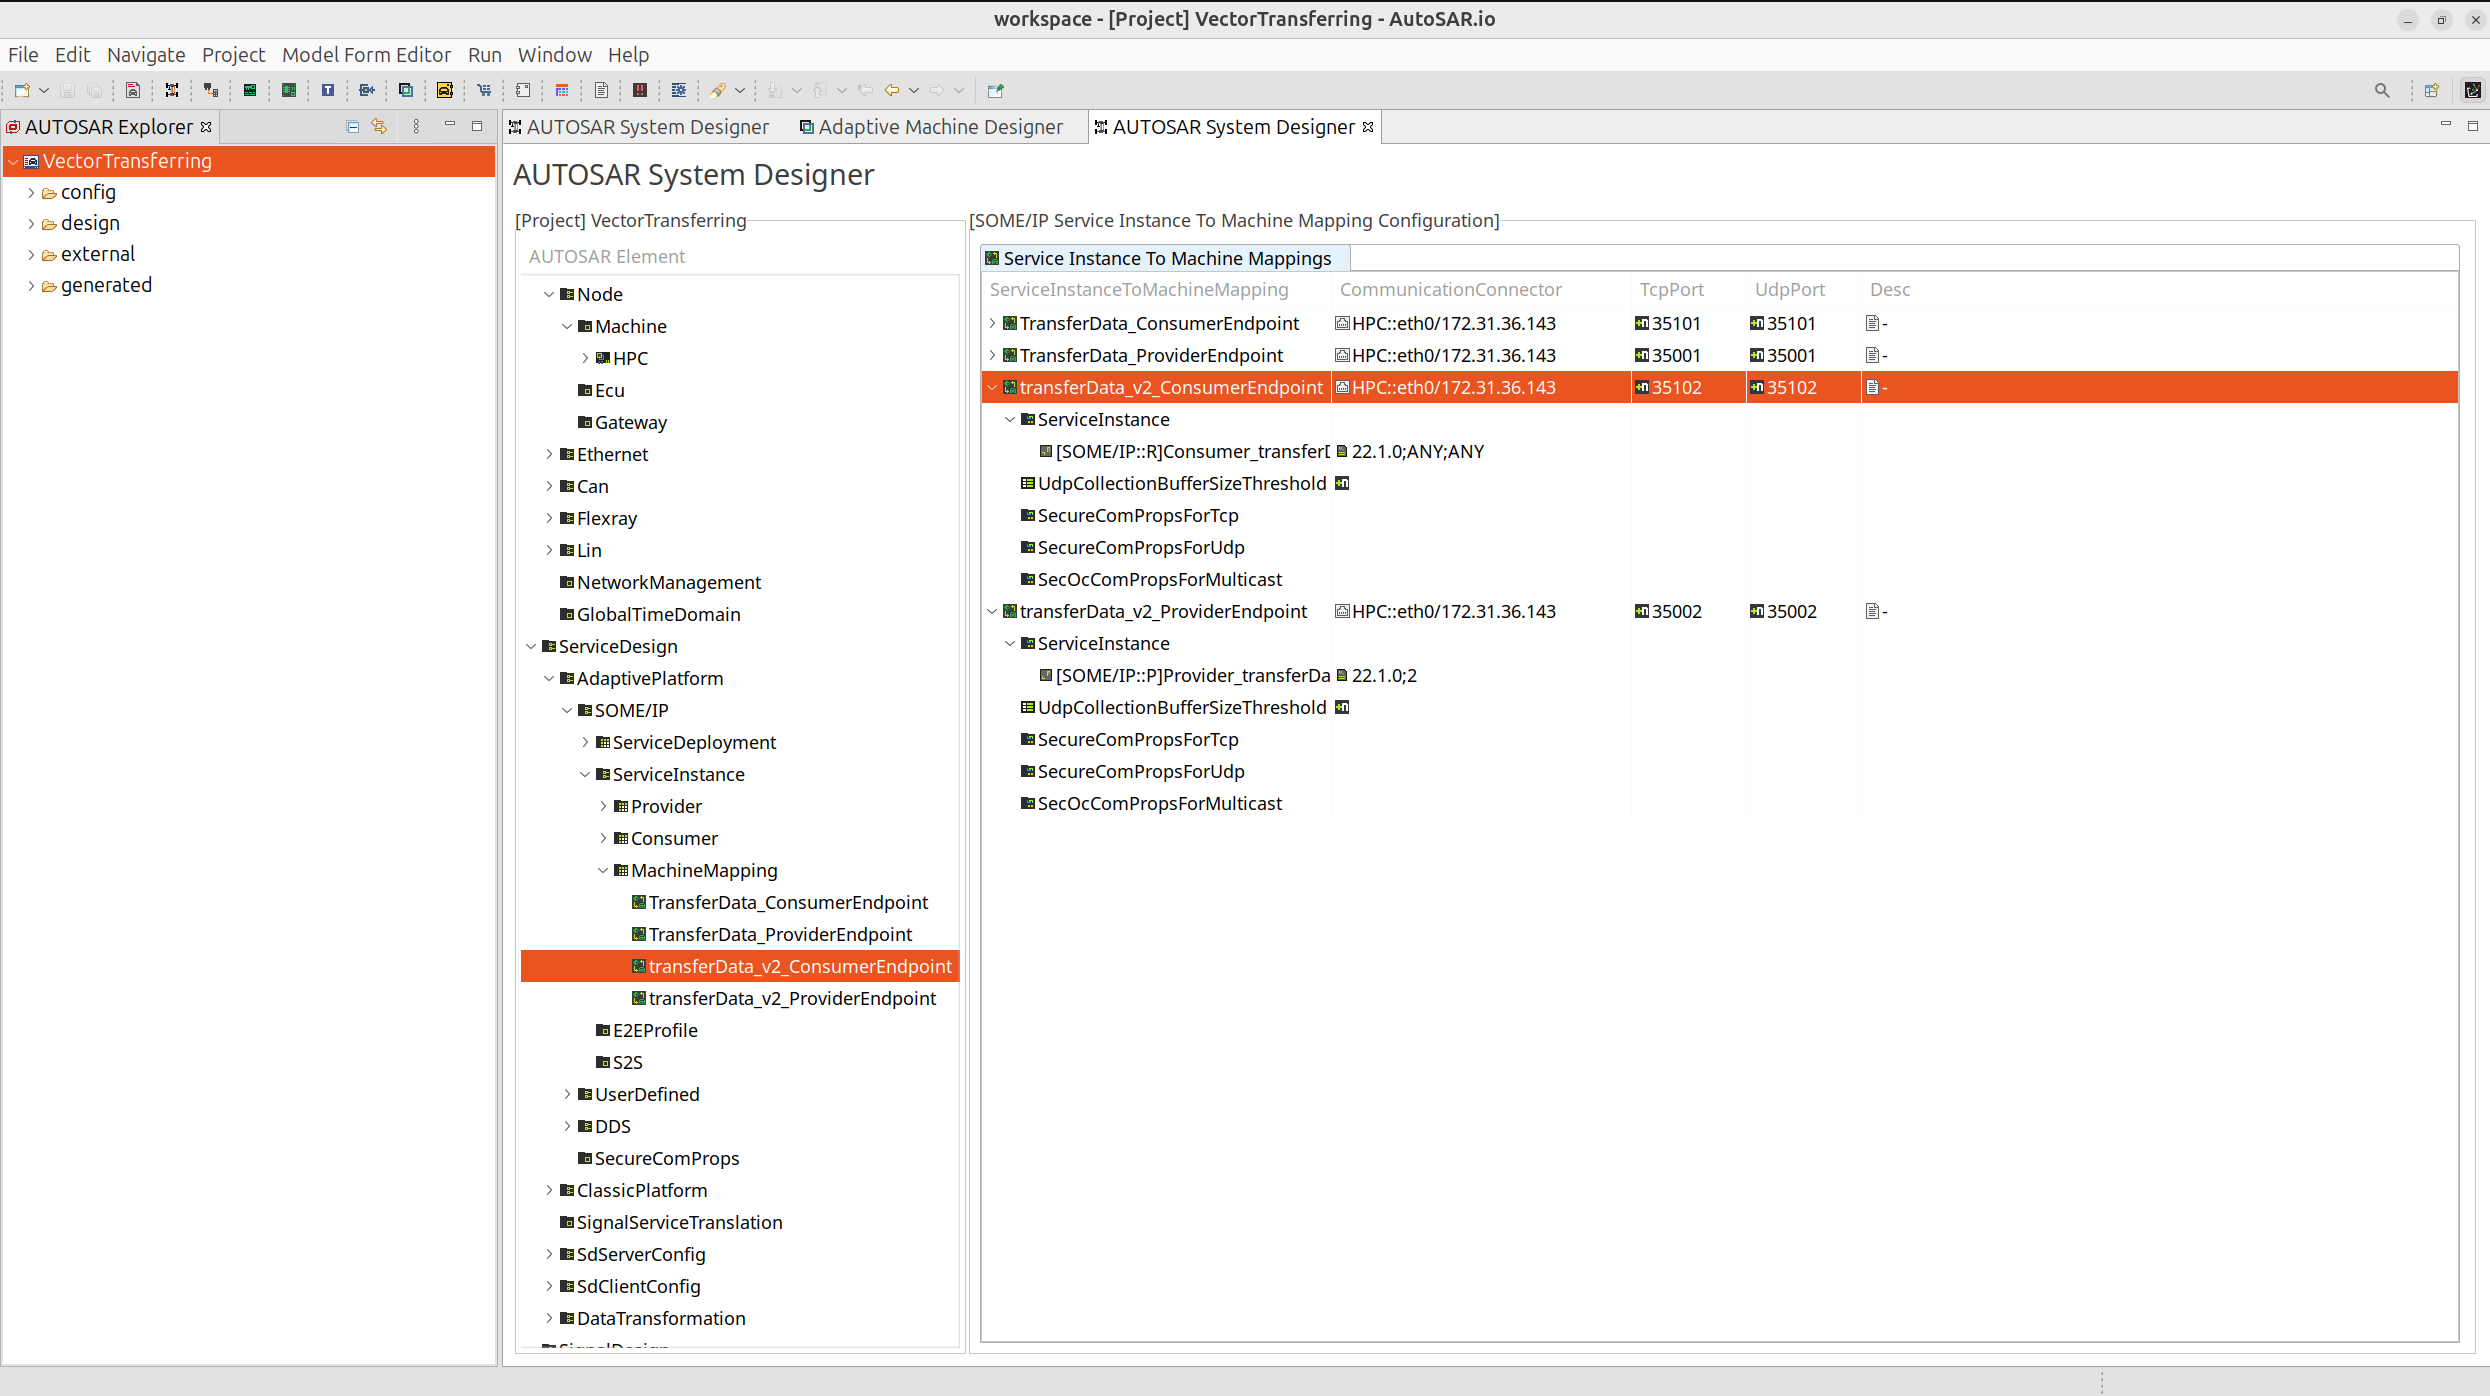
\includegraphics[width=0.75\textwidth]{Images/chap3/image_methodology/serviceInterfaceDesign/serviceMappingMachineEndpoint.png}
    \vspace{0.5cm}
    \caption{Mapping Service Instances to Machine Network Endpoint}
    \label{fig:service_machine_endpoint_mapping}
\end{figure}

Figure~\ref{fig:service_machine_endpoint_mapping} illustrates how the service instances of the \texttt{transferData} and \texttt{transferData\_v2} interfaces are bound to concrete machine network endpoints. Both provider and consumer instances are mapped to the Ethernet communication connector \texttt{HPC:eth0} with the fixed IPv4 address \texttt{172.31.36.143}, ensuring that all service communication is routed through a well defined network interface. Distinct TCP and UDP port numbers are assigned to each service instance, allowing concurrent data exchange while avoiding port conflicts.

This mapping explicitly links abstract service definitions to physical network resources, enabling correct runtime deployment and communication over SOME/IP. By defining separate endpoints for provider and consumer roles, the configuration supports clear role separation and reliable message routing between applications deployed on the same machine or across different nodes in the Adaptive AUTOSAR system.

\begin{figure}[H]
    \centering
    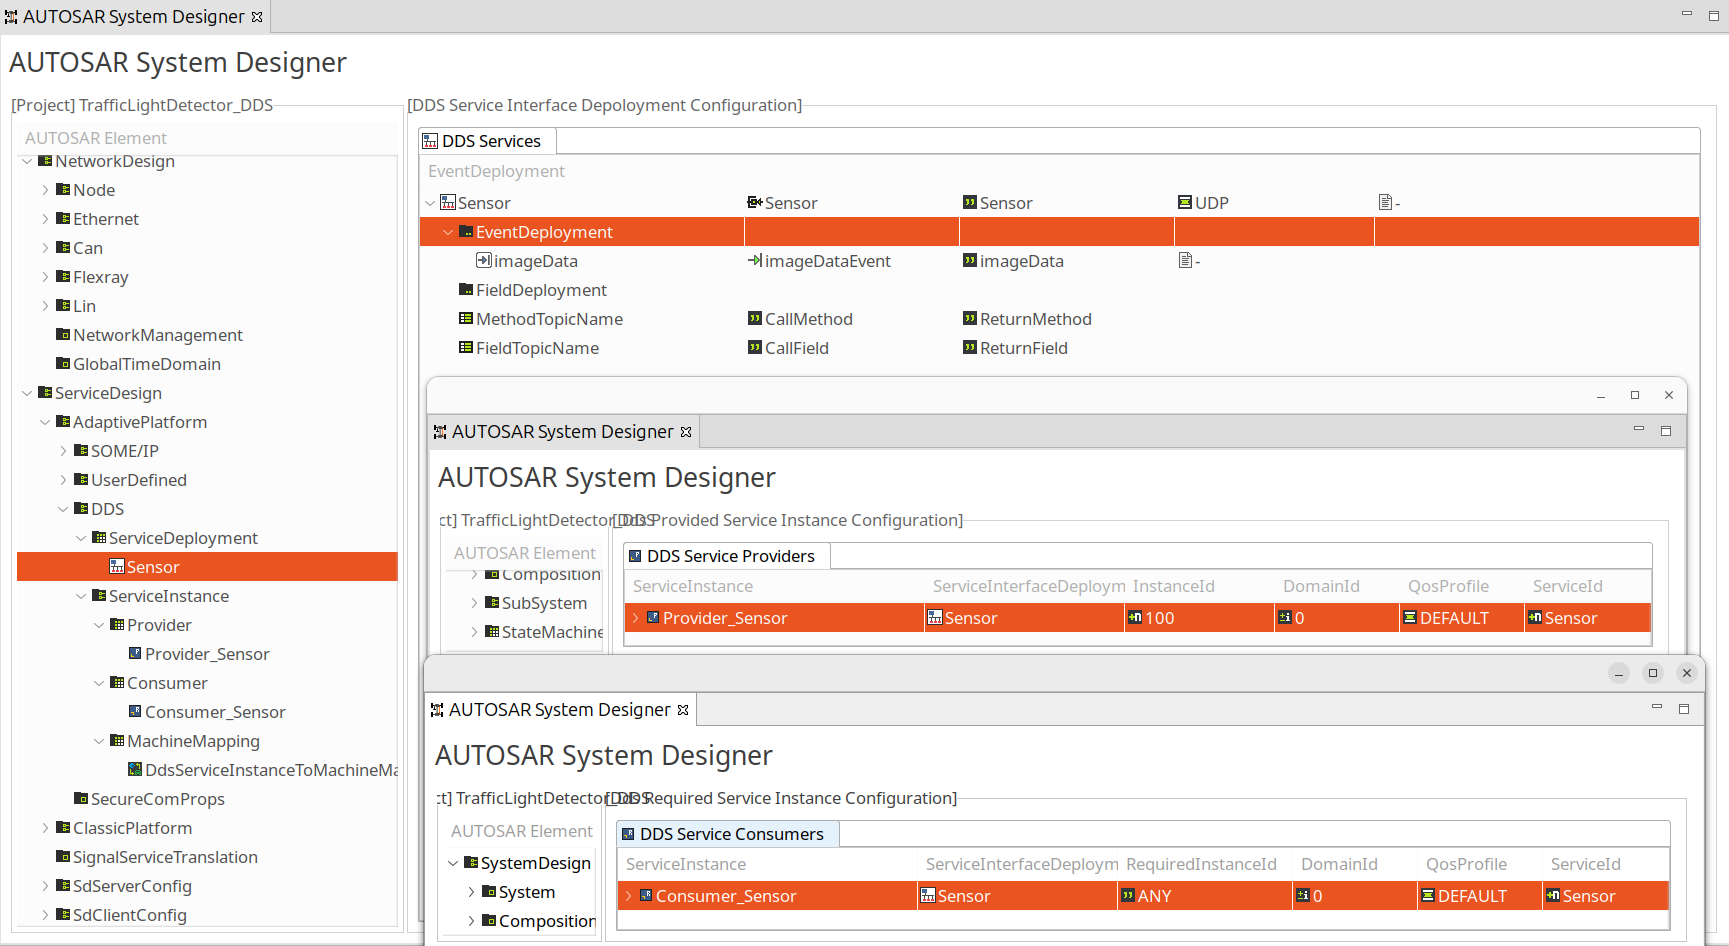
\includegraphics[width=0.75\textwidth]{Images/chap3/image_methodology/serviceInterfaceDesign/DDS_Config.png}
    \vspace{0.5cm}
    \caption{Mapping Service Instances to Machine Network Endpoint}
    \label{fig:dds_config}
\end{figure}

Similarly to the SOME/IP configuration, Figure~\ref{fig:dds_config} presents the DDS-based deployment configuration used for the \texttt{Sensor} service. In the DDS Service Interface Deployment Configuration, the service interface is deployed with the \texttt{imageDataEvent} event and the corresponding DDS topic \texttt{imageData}. The event deployment is configured to use UDP transport, allowing the Provider and Client applications to exchange image and metadata payloads through DDS publish/subscribe communication.

The provided service instance is configured as \texttt{Provider\_Sensor}, bound to the \texttt{Sensor} service deployment with instance-id~\texttt{100}, DDS Domain Id~\texttt{0}, and the \texttt{DEFAULT} QoS profile. The required service instance is configured as \texttt{Consumer\_Sensor}, also bound to the same \texttt{Sensor} service deployment, but with required instance-id~\texttt{ANY}. This configuration allows the Client application to discover and subscribe to the Provider service instance dynamically within the same DDS domain.

Through this DDS configuration, the abstract AUTOSAR service definition is mapped to concrete DDS communication entities, including service deployment, topic, event, provider instance, consumer instance, domain identifier, and QoS profile. This mapping is essential for the implemented prototype because the runtime communication between \texttt{ProviderSensor} and \texttt{ClientSensor} is realized through DDS rather than SOME/IP. As a result, the system can publish \texttt{imageDataEvent} samples on the \texttt{imageData} topic and deliver the \texttt{GpsJpegWireHeader + JPEG} payload from the Provider to the Client in a service-oriented and configurable manner.

\subsubsection{Application Design}

% Modeling Adaptive Application
\begin{figure}[H]
    \centering
    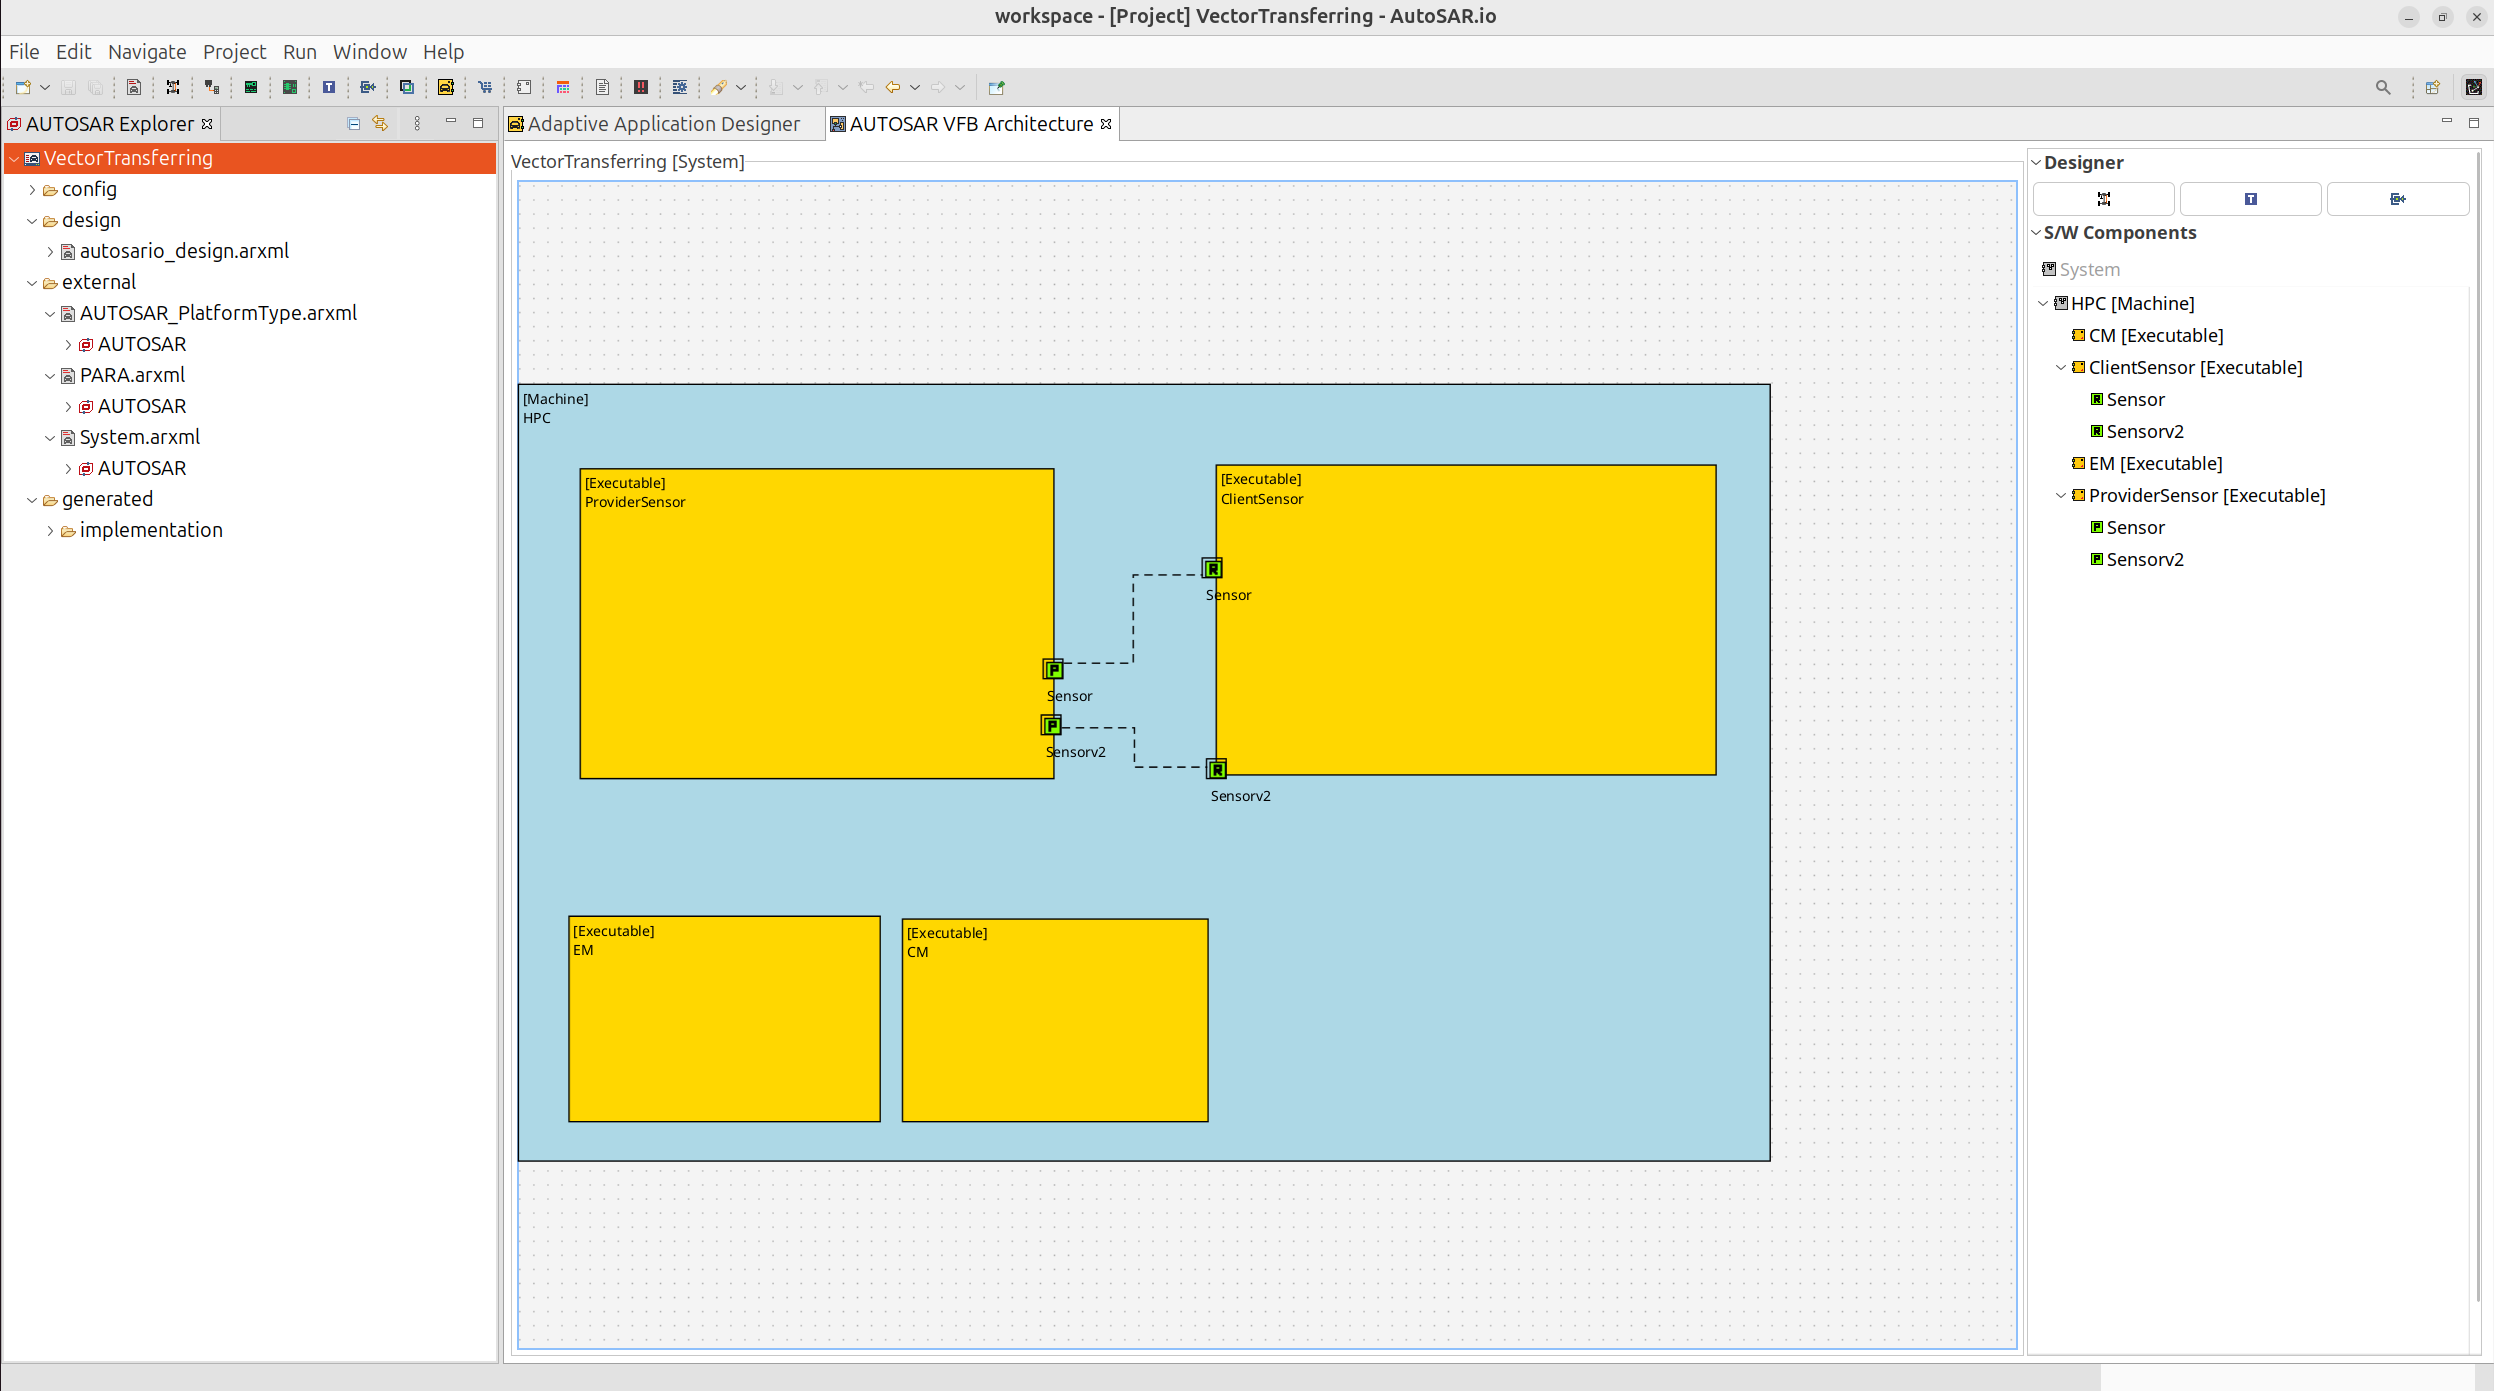
\includegraphics[width=0.75\textwidth]{Images/chap3/image_methodology/applicationDesign/modelingApplication.png}
    \vspace{0.5cm}
    \caption{Modeling of Adaptive Application}
    \label{fig:modeling_application}
\end{figure}

Figure~\ref{fig:modeling_application} shows the Adaptive Application modeling view, where users define the overall application architecture by assigning application executables to a specific machine. In this workspace, the target machine \texttt{HPC} is selected as the deployment context, and multiple executables such as \texttt{ProviderSensor}, \texttt{ClientSensor}, \texttt{CM}, and \texttt{EM} are instantiated within it. Logical connections between executables are visually represented through ports, allowing designers to describe interaction relationships at the architectural level. This model serves as a central design step that links application executables with the underlying machine, providing a clear and structured representation of how software components are organized and deployed in an Adaptive AUTOSAR system.


% Configure Provider Executable Properties
\begin{figure}[H]
    \centering
    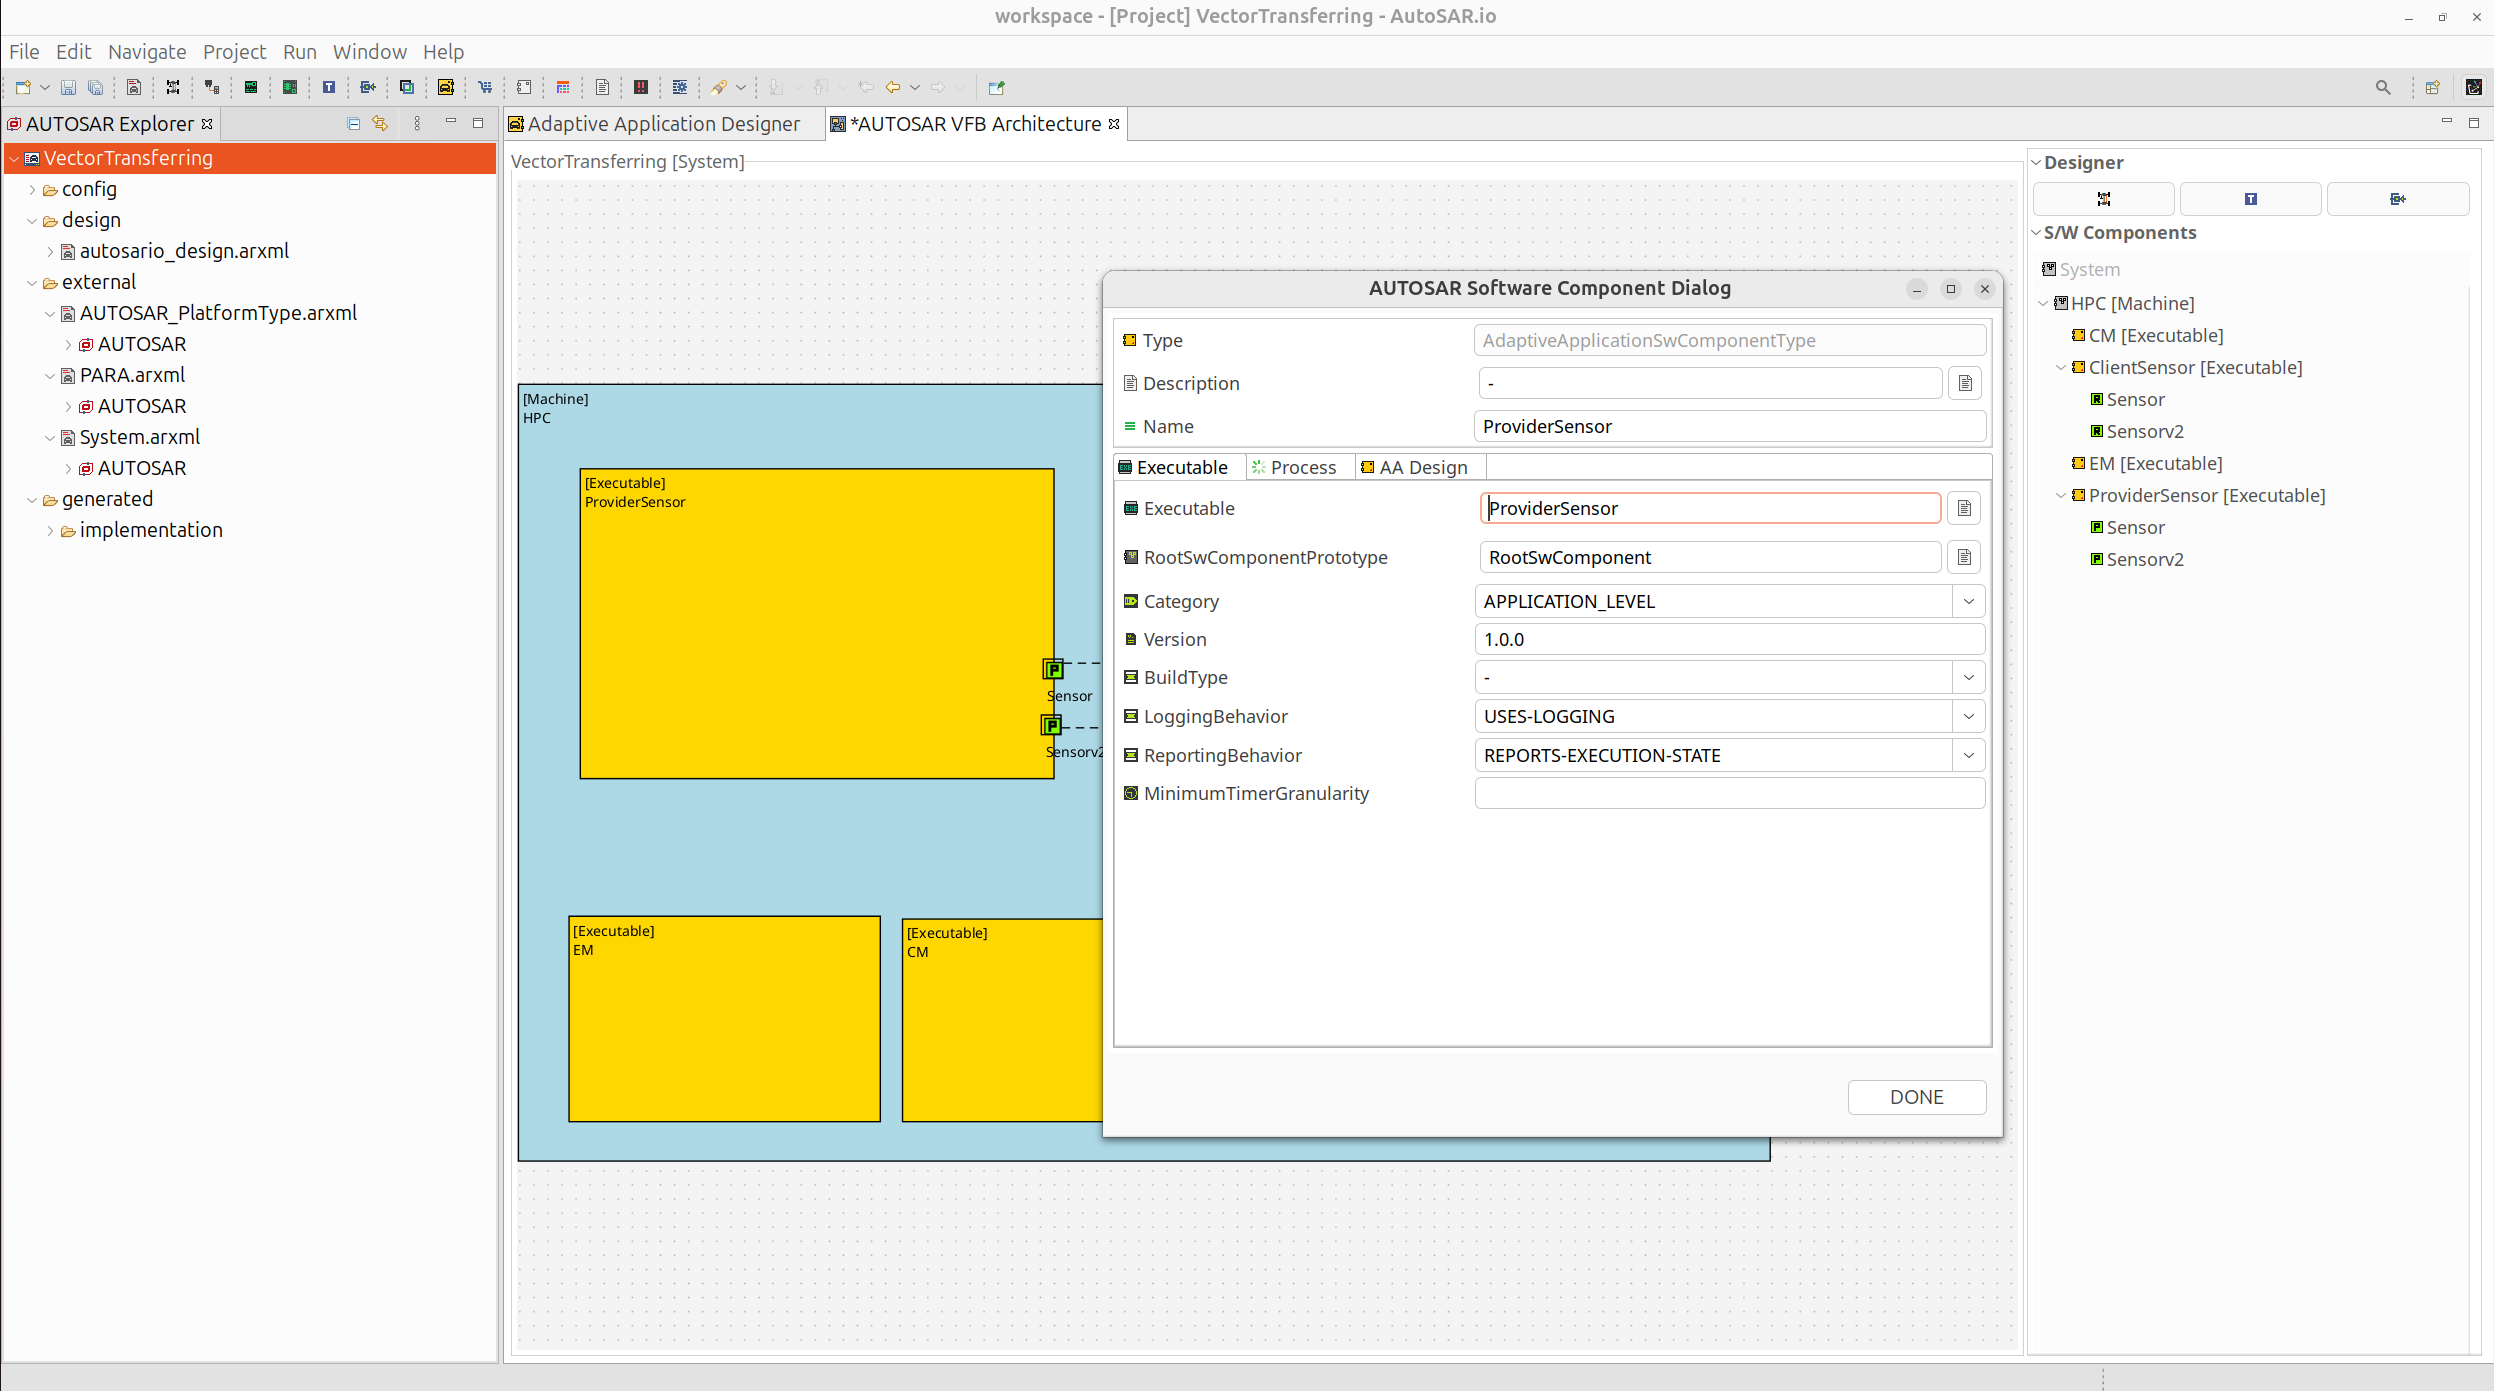
\includegraphics[width=0.75\textwidth]{Images/chap3/image_methodology/applicationDesign/providerExProperties.png}
    \vspace{0.5cm}
    \caption{Configuration of Provider Executable Properties}
    \label{fig:app_provider_executable_properties}
\end{figure}

Figure~\ref{fig:app_provider_executable_properties} presents the configuration of the provider application executable within the Adaptive Application Designer. In this view, the executable \texttt{ProviderSensor} is defined as an application level software component with a specific version and logging behavior. Key properties such as execution category, reporting behavior, and minimum timer granularity are configured to control runtime characteristics and observability. By assigning these attributes, the provider executable is clearly identified as a service offering entity and is prepared to integrate with the Adaptive AUTOSAR execution environment in a consistent and manageable manner.

% Map Provider Ports to Service Interface
\begin{figure}[H]
    \centering
    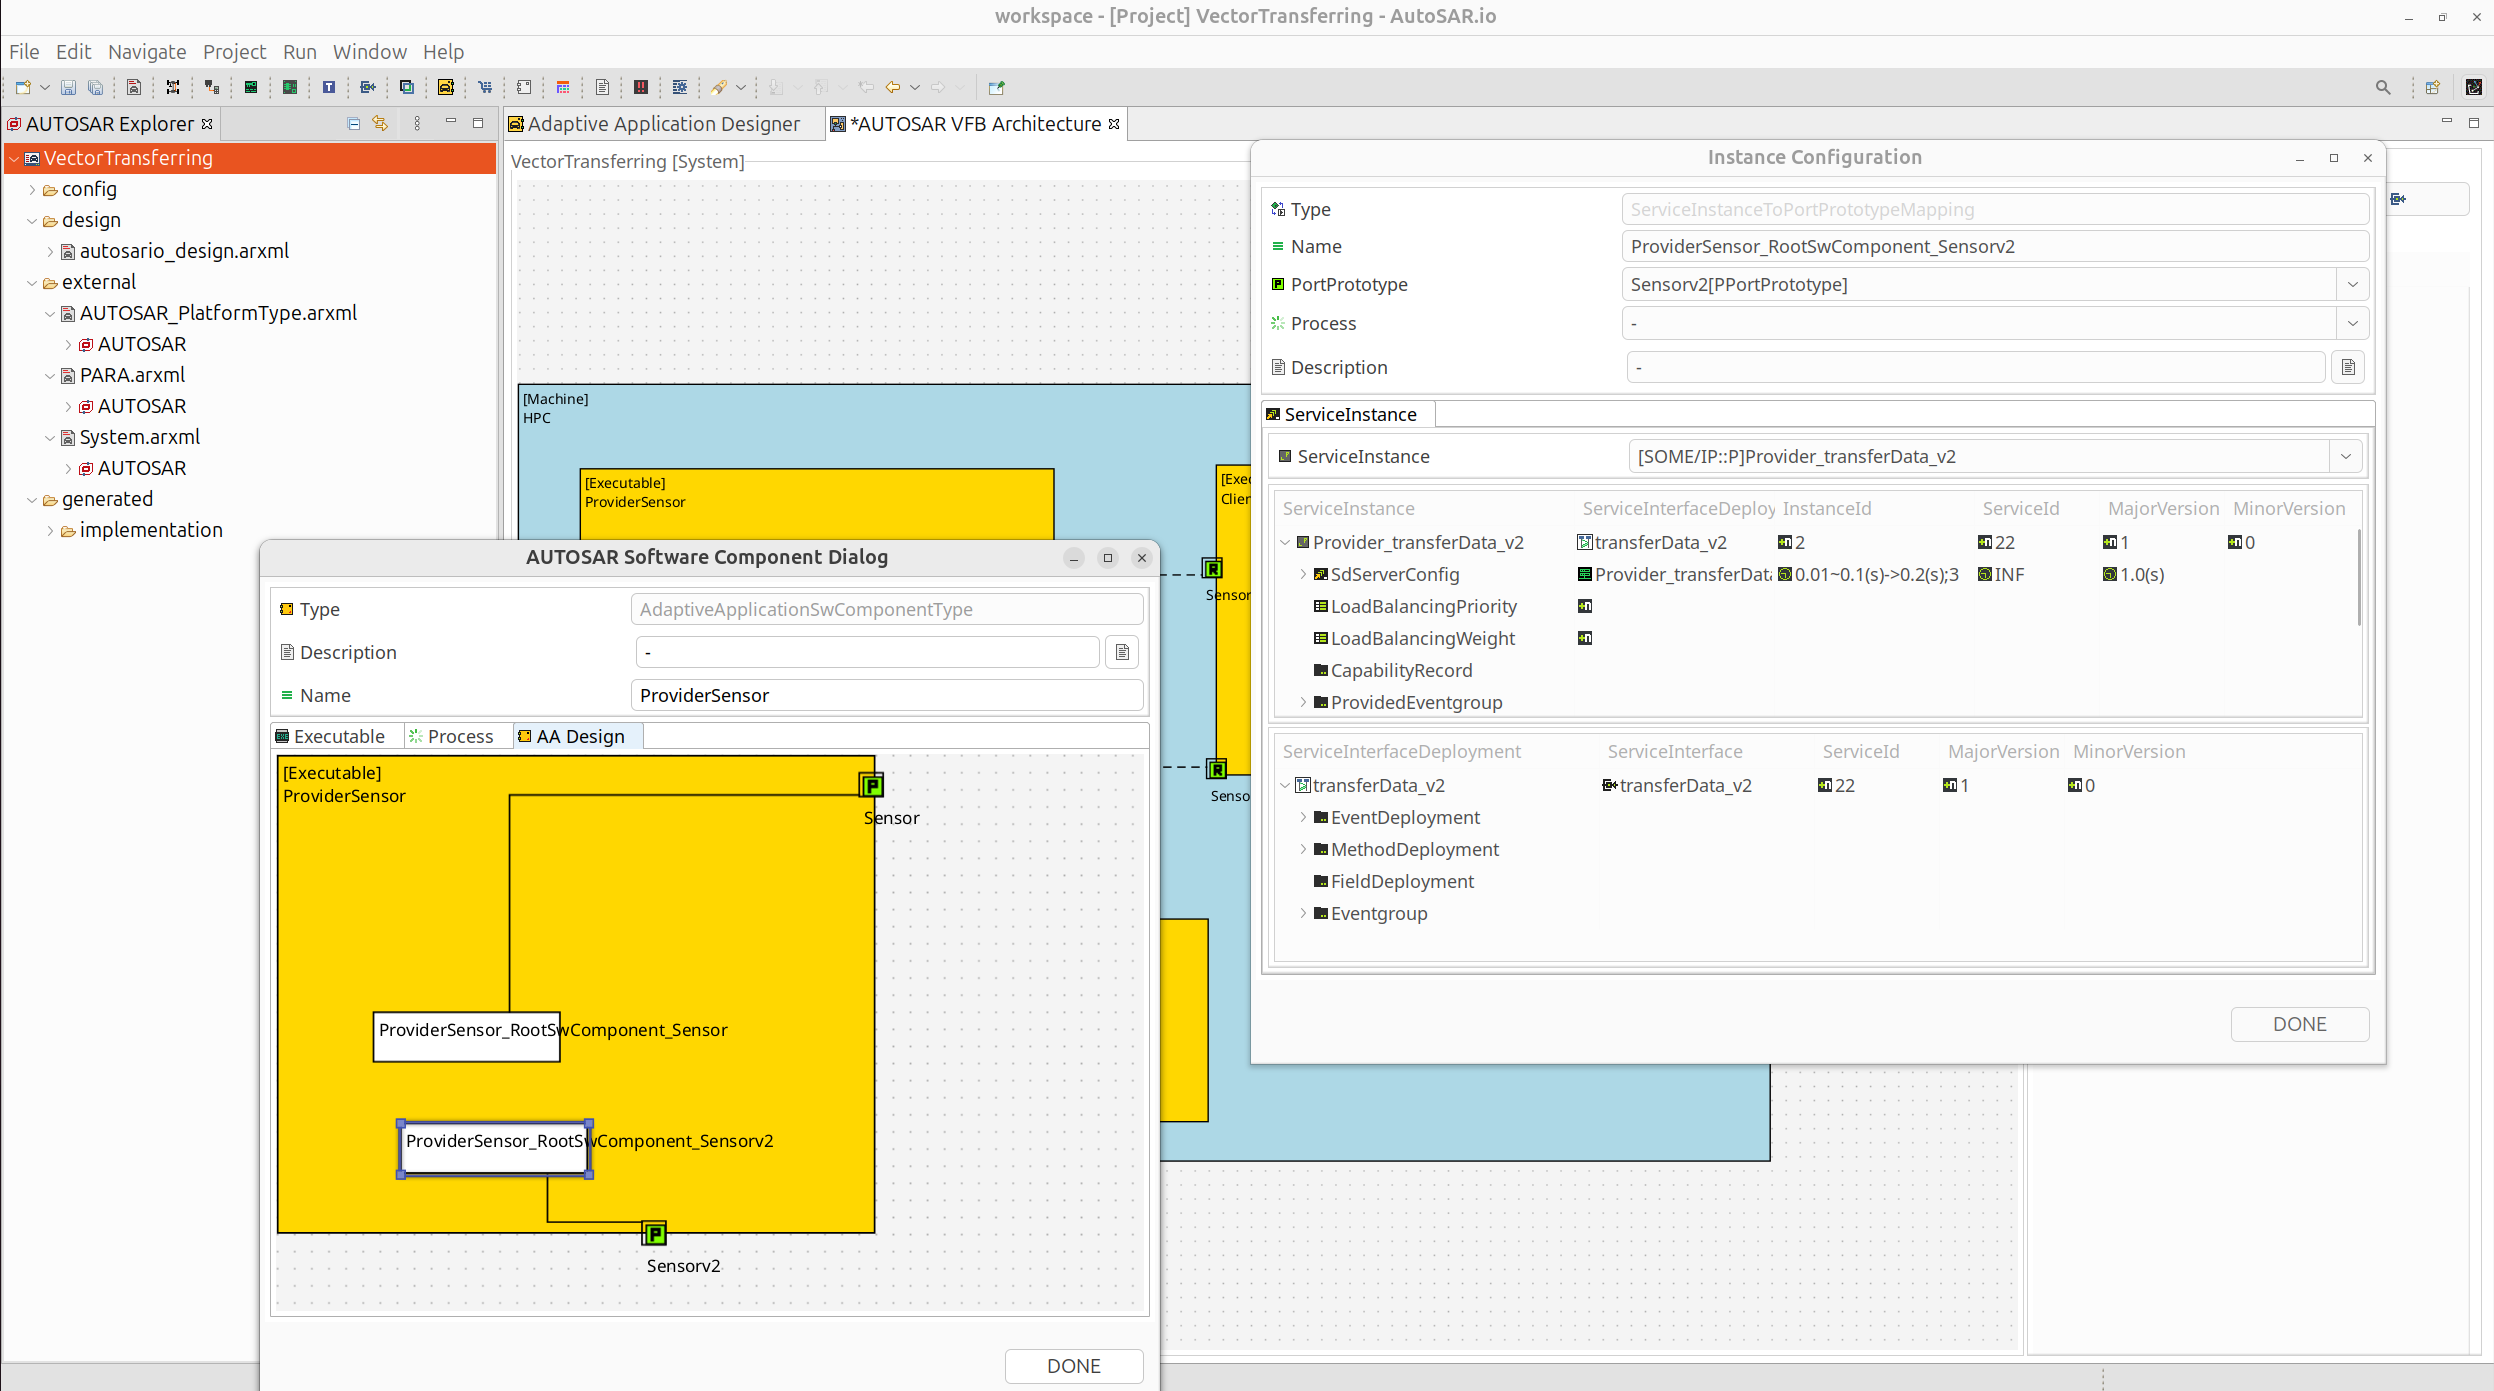
\includegraphics[width=0.75\textwidth]{Images/chap3/image_methodology/applicationDesign/mappingPortProviderEx.png}
    \vspace{0.5cm}
    \caption{Mapping Provider Ports to Service Interface}
    \label{fig:app_mapping_provider_ports}
\end{figure}

Figure~\ref{fig:app_mapping_provider_ports} illustrates the association between the provider executable ports and the previously defined AUTOSAR software component. In this step, the ports of the \texttt{ProviderSensor} executable are mapped to the corresponding port prototypes of the Adaptive Application Software Component that has already been specified in the AUTOSAR model. This configuration establishes a clear link between the executable instance and its software component definition, ensuring that the executable correctly realizes the component’s provided interfaces. As a result, the application implementation becomes consistent with the AUTOSAR architectural model before being bound to concrete service instances and communication middleware.


% Configure Subscriber Executable Properties
\begin{figure}[H]
    \centering
    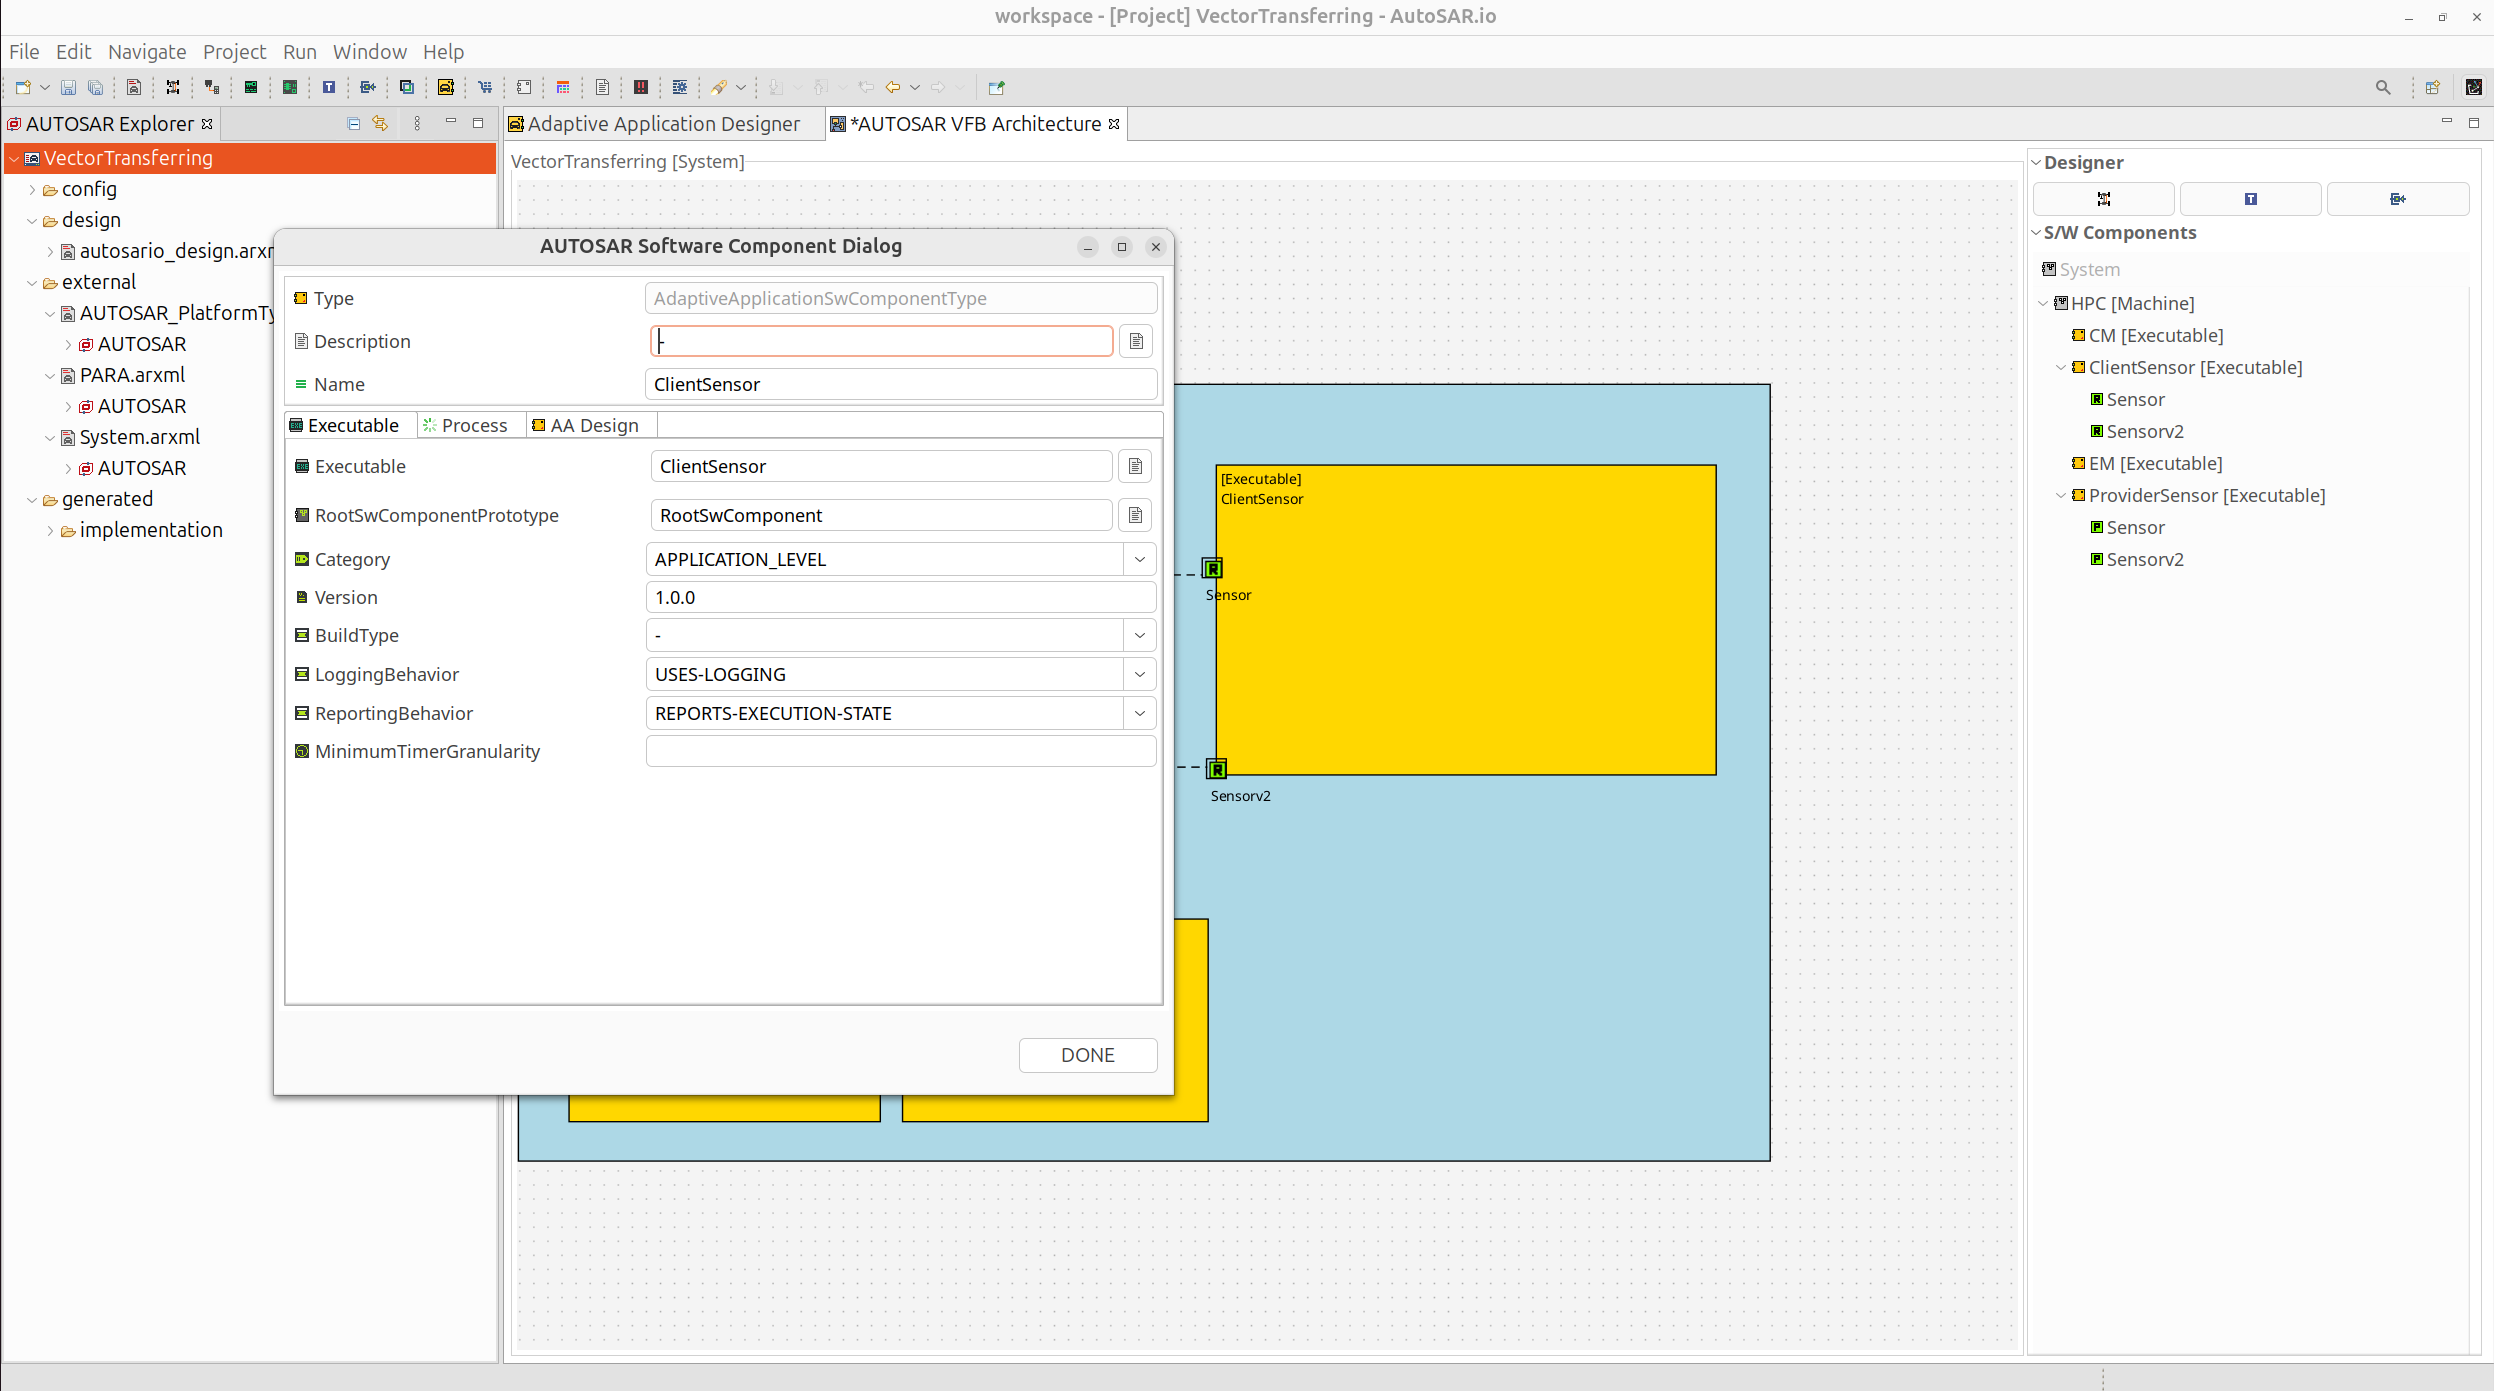
\includegraphics[width=0.75\textwidth]{Images/chap3/image_methodology/applicationDesign/subscriberExProperties.png}
    \vspace{0.5cm}
    \caption{Configuration of Subscriber Executable Properties}
    \label{fig:app_subscriber_executable_properties}
\end{figure}

Figure~\ref{fig:app_subscriber_executable_properties} illustrates the definition of the \texttt{ClientSensor} executable as an adaptive application software component. In this step, the executable is characterized at the application level by specifying its name, version, category, and runtime behavior such as logging and execution state reporting. This configuration formally registers the client application in the AUTOSAR model and establishes it as a runnable entity that can participate in service oriented communication.

% Map Client Ports to Service Interface
\begin{figure}[H]
    \centering
    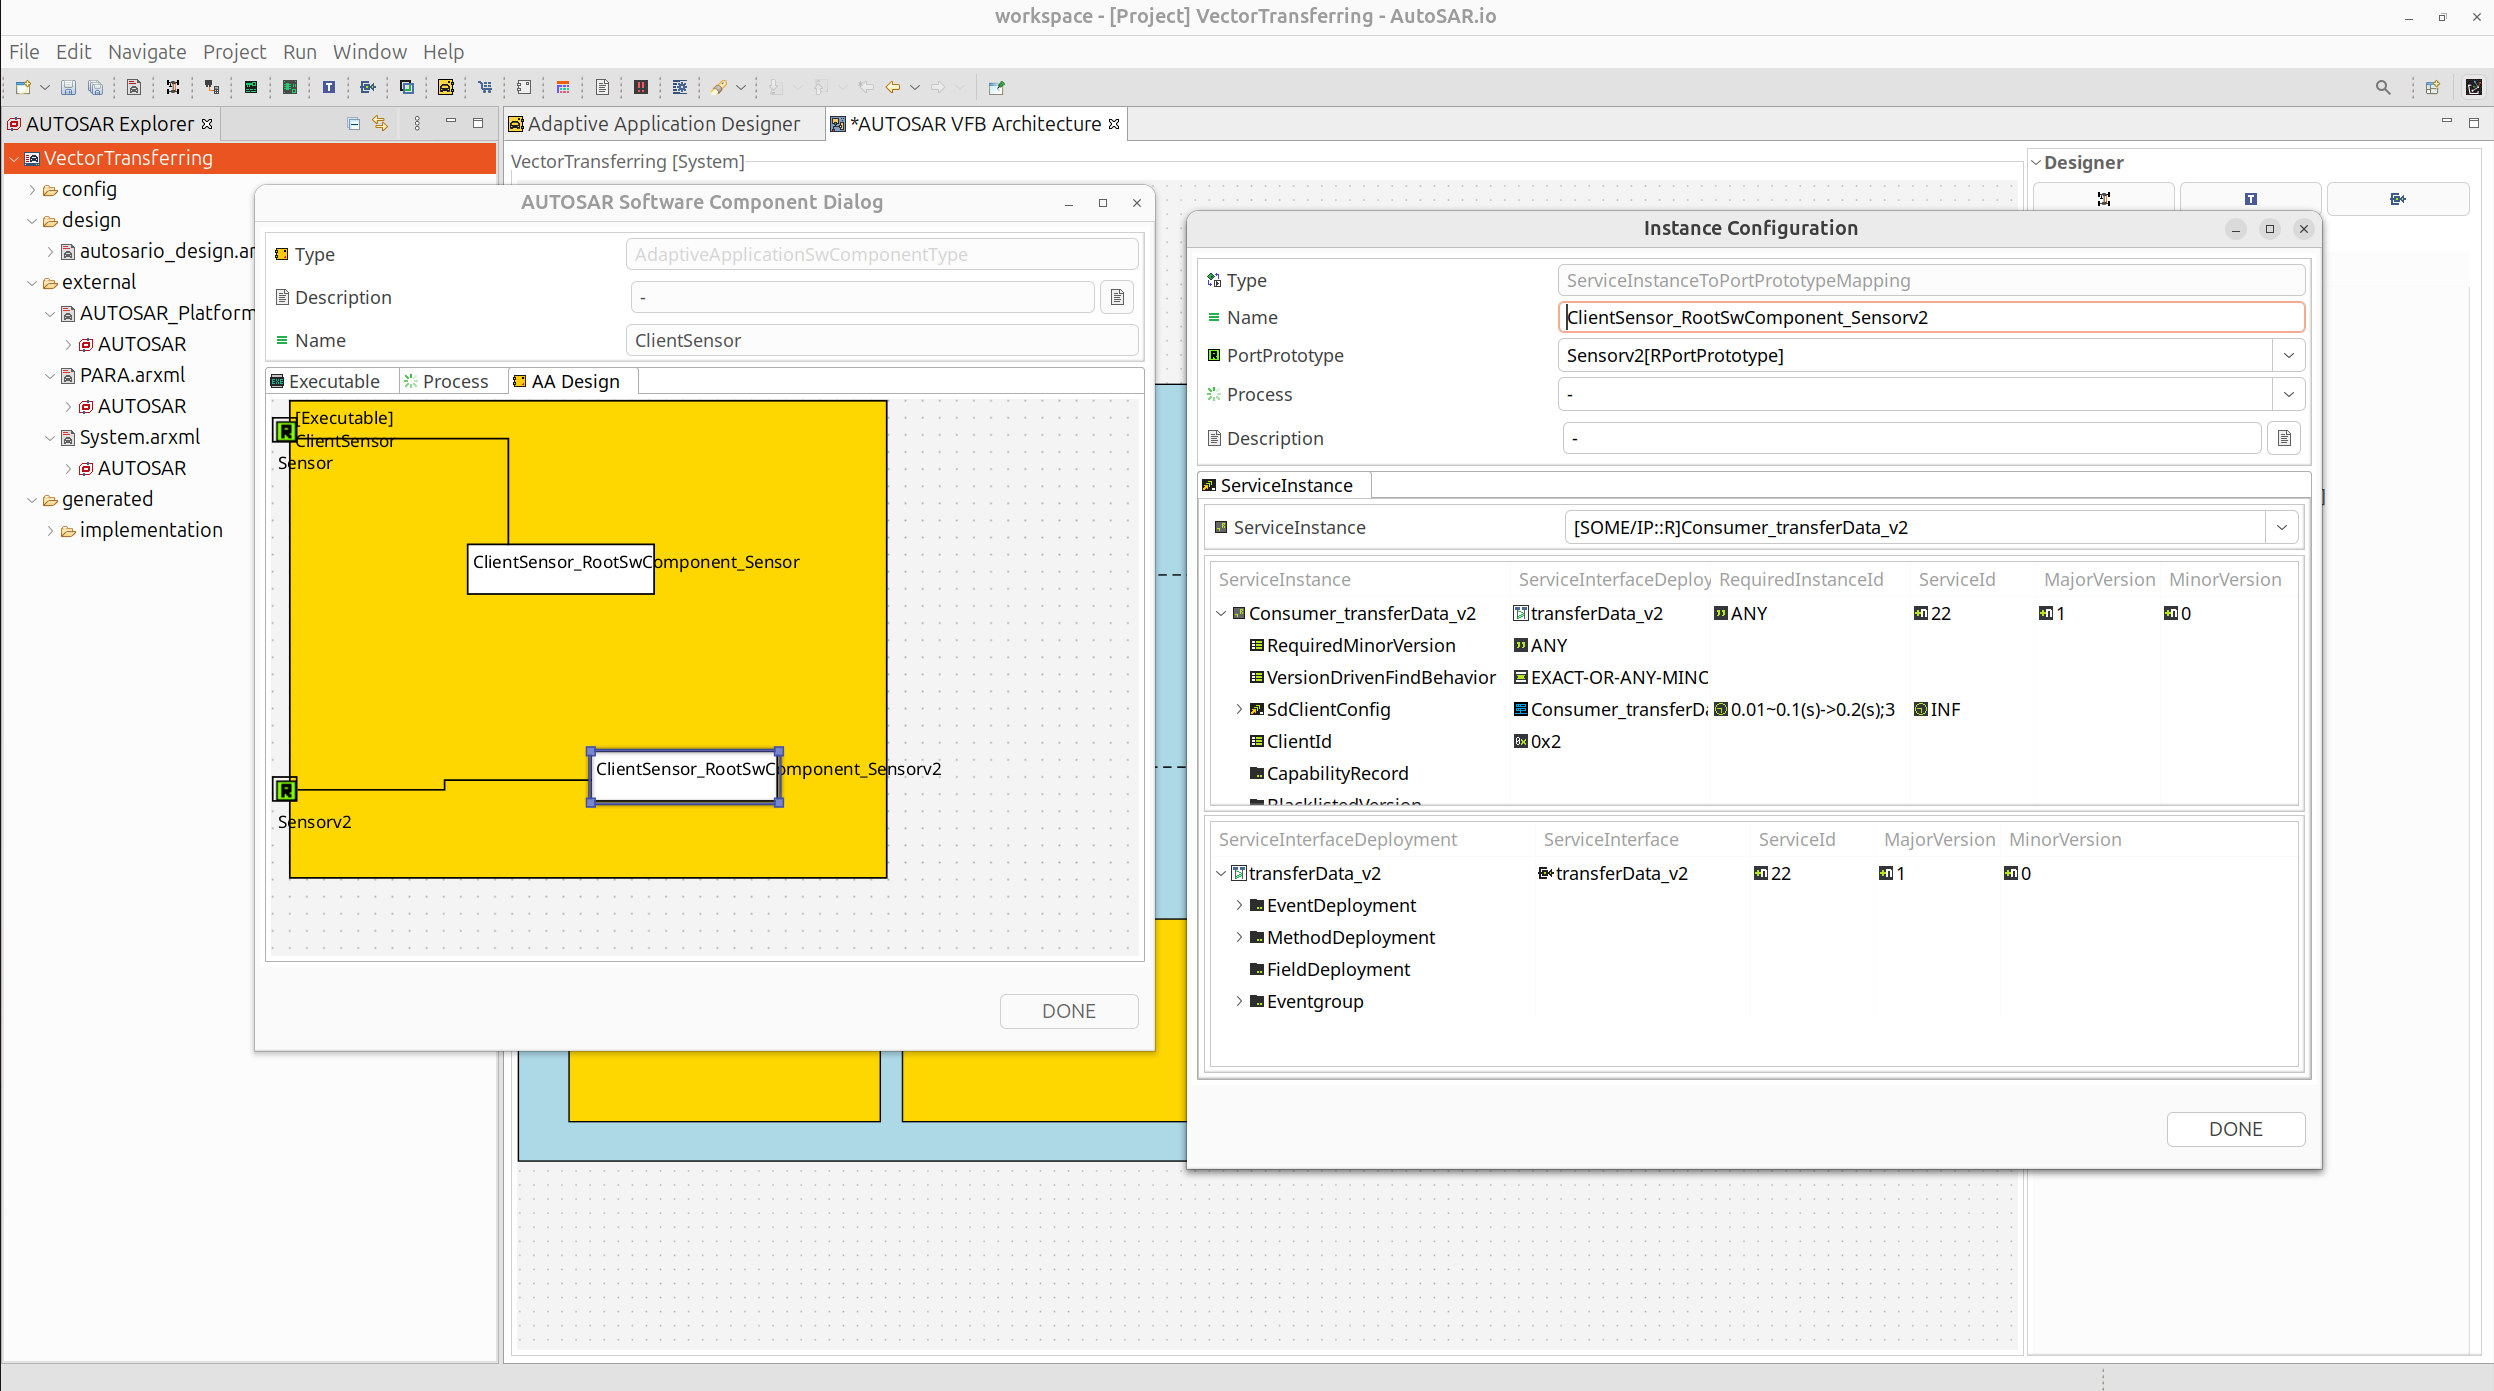
\includegraphics[width=0.75\textwidth]{Images/chap3/image_methodology/applicationDesign/mappingPortClientEx.png}
    \vspace{0.5cm}
    \caption{Mapping Client Ports to Service Interface}
    \label{fig:app_mapping_client_ports}
\end{figure}

As shown in Figure~\ref{fig:app_mapping_client_ports}, the required ports of the \texttt{ClientSensor} software component are then associated with the corresponding port prototypes defined in the AUTOSAR architecture. This association links the client implementation to the abstract interface contracts specified at design time, without directly binding it to network level details. By completing this step, the client executable is structurally aligned with the AUTOSAR software component model, enabling subsequent binding to concrete service instances during service deployment and machine mapping.

% Configure Application Startup Behavior
\begin{figure}[H]
    \centering
    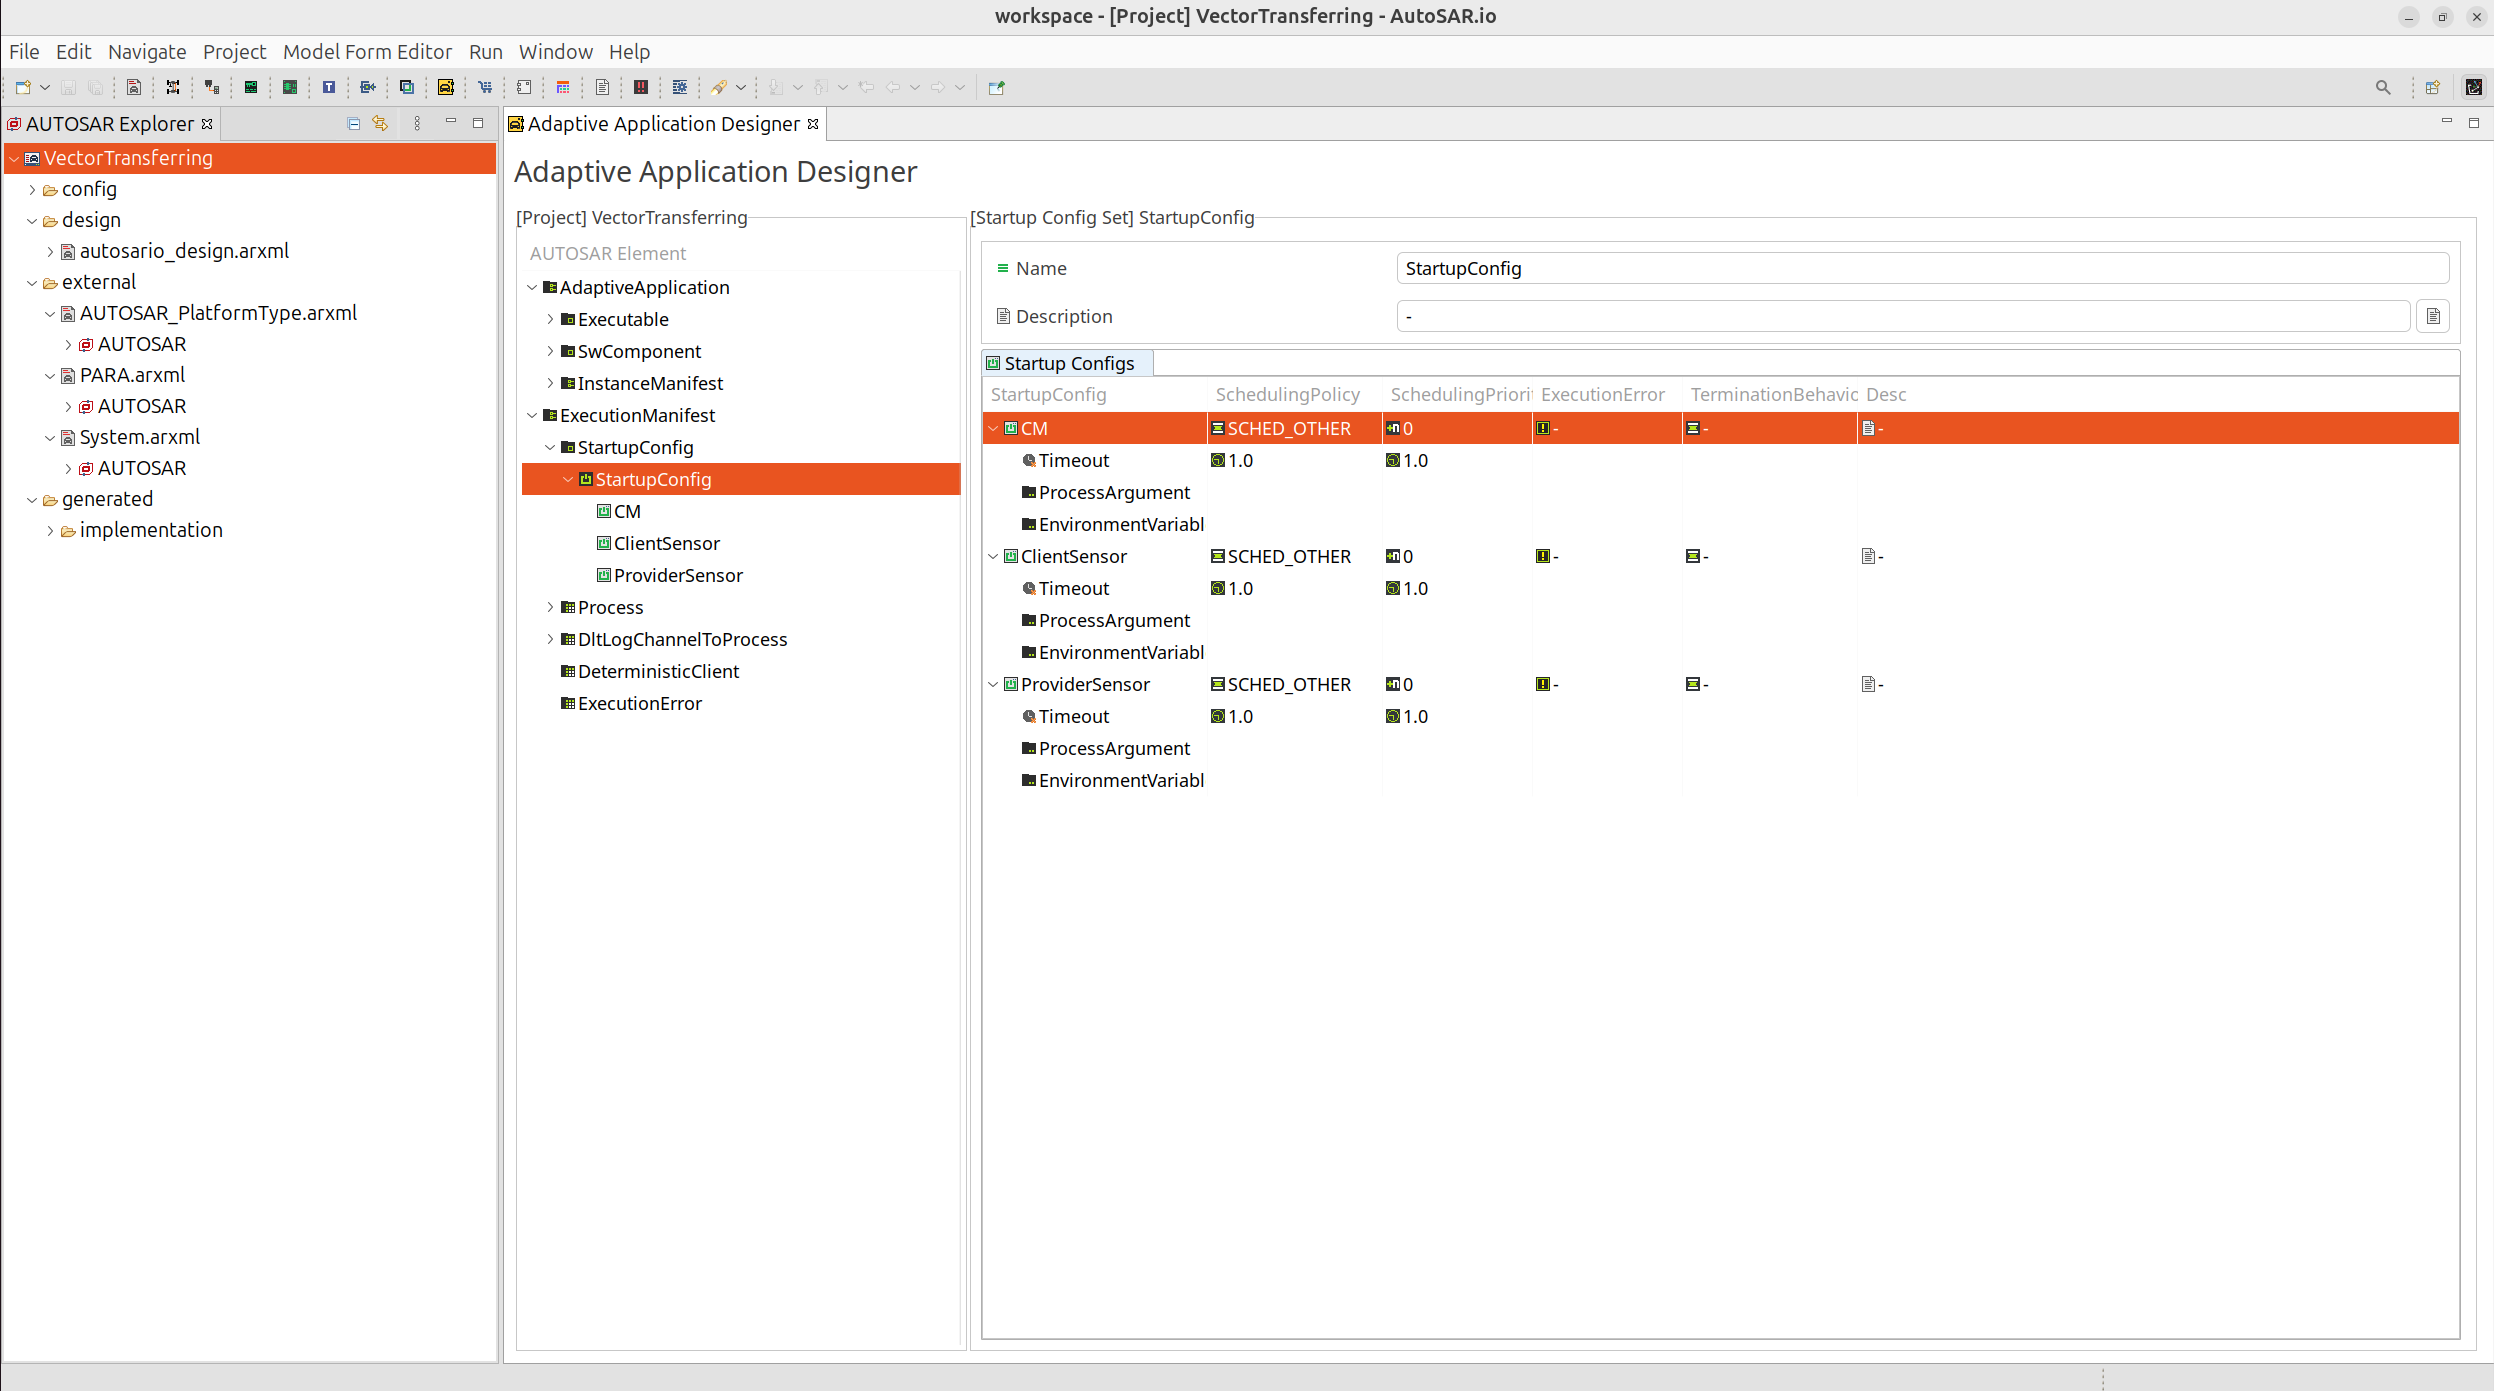
\includegraphics[width=0.75\textwidth]{Images/chap3/image_methodology/applicationDesign/configureStartupConfigure.png}
    \vspace{0.5cm}
    \caption{Configuration of Application Startup Behavior}
    \label{fig:app_startup_configuration}
\end{figure}

Figure~\ref{fig:app_startup_configuration} illustrates the startup configuration set that governs how adaptive application processes are initialized on the target platform. Each process, including \texttt{CM}, \texttt{ClientSensor}, and \texttt{ProviderSensor}, is assigned a scheduling policy and priority, ensuring consistent execution behavior under the POSIX based operating environment. The use of a unified scheduling class allows the platform to manage multiple applications in a predictable manner during system boot.

In addition, the startup configuration defines timeout values and process level parameters that control execution supervision at launch time. By explicitly specifying these attributes, the system ensures that all applications enter a well defined initial state and comply with platform execution constraints. This configuration plays a critical role in coordinating application startup with function group transitions and provides a stable foundation for subsequent runtime interactions.

% Bind DLT Channels to Application Processes
\begin{figure}[H]
    \centering
    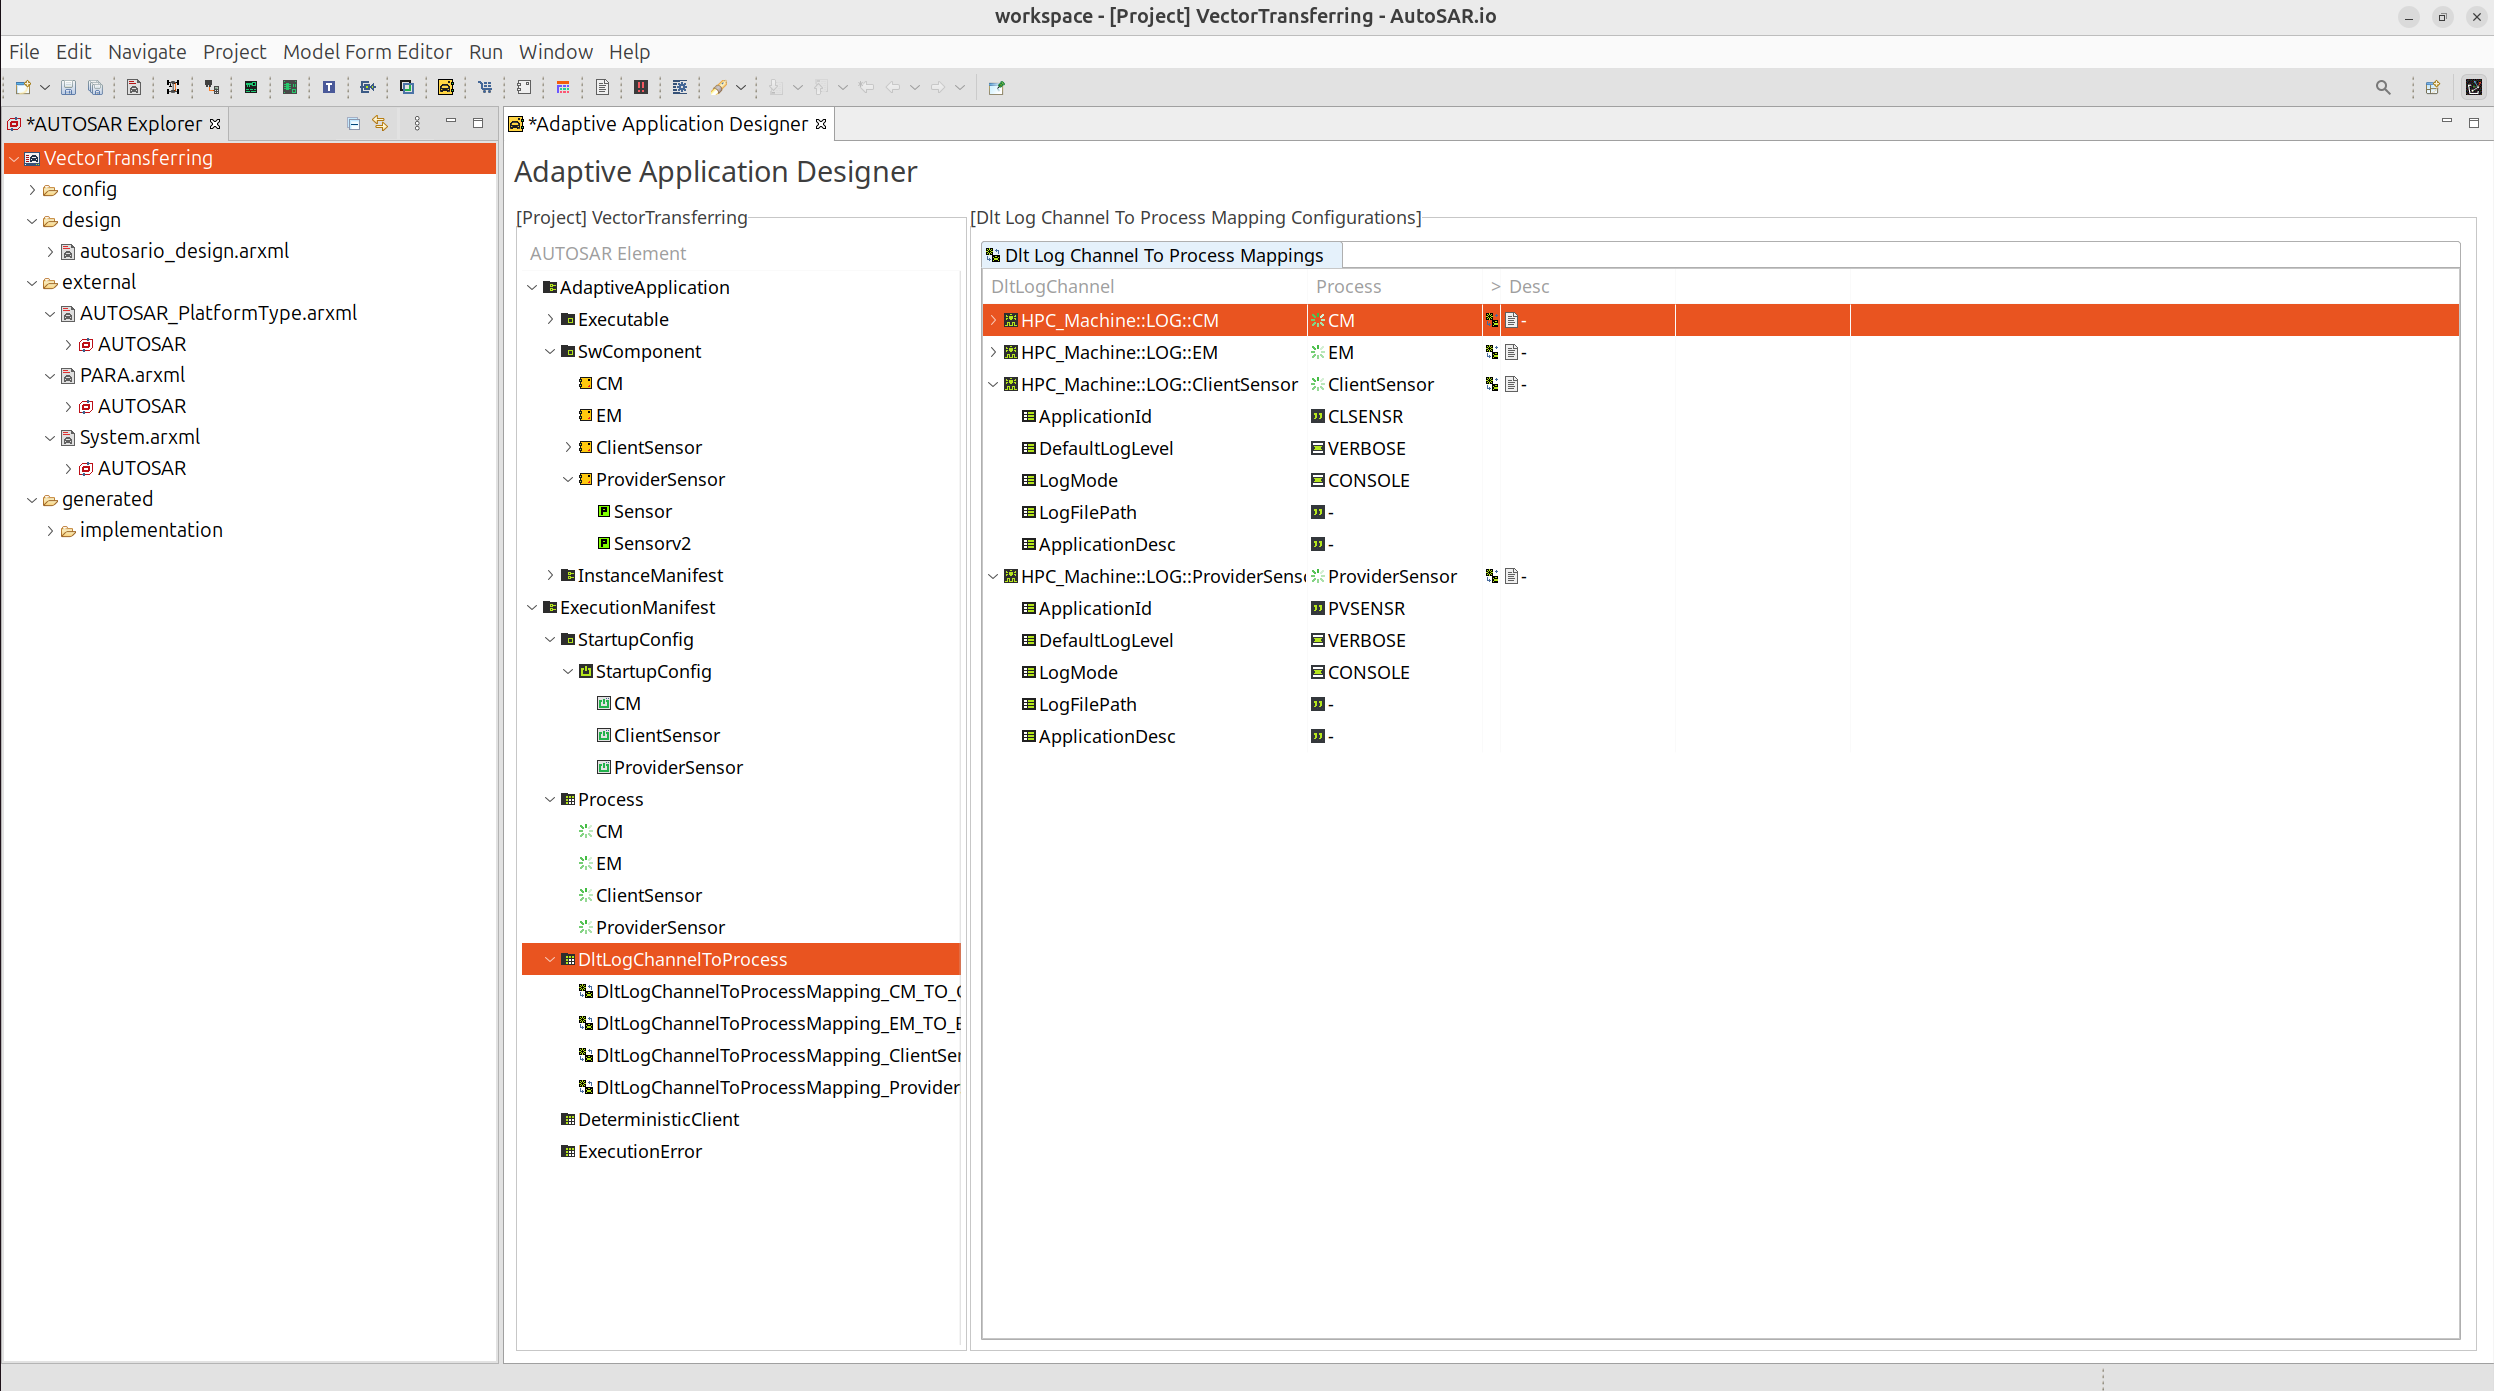
\includegraphics[width=0.75\textwidth]{Images/chap3/image_methodology/applicationDesign/configureDLTChanneltoProcess.png}
    \vspace{0.5cm}
    \caption{Binding Diagnostic Log and Trace Channels to Application Processes}
    \label{fig:app_dlt_process_mapping}
\end{figure}

Figure~\ref{fig:app_dlt_process_mapping} depicts the association between Diagnostic Log and Trace channels and individual application processes. Each process is connected to a specific DLT channel with defined log levels and output modes, enabling consistent monitoring and debugging at runtime. This mapping ensures that diagnostic information is traceable per application, which supports efficient analysis and maintenance in Adaptive AUTOSAR deployments.

% Configure Provider Application Process
\begin{figure}[H]
    \centering
    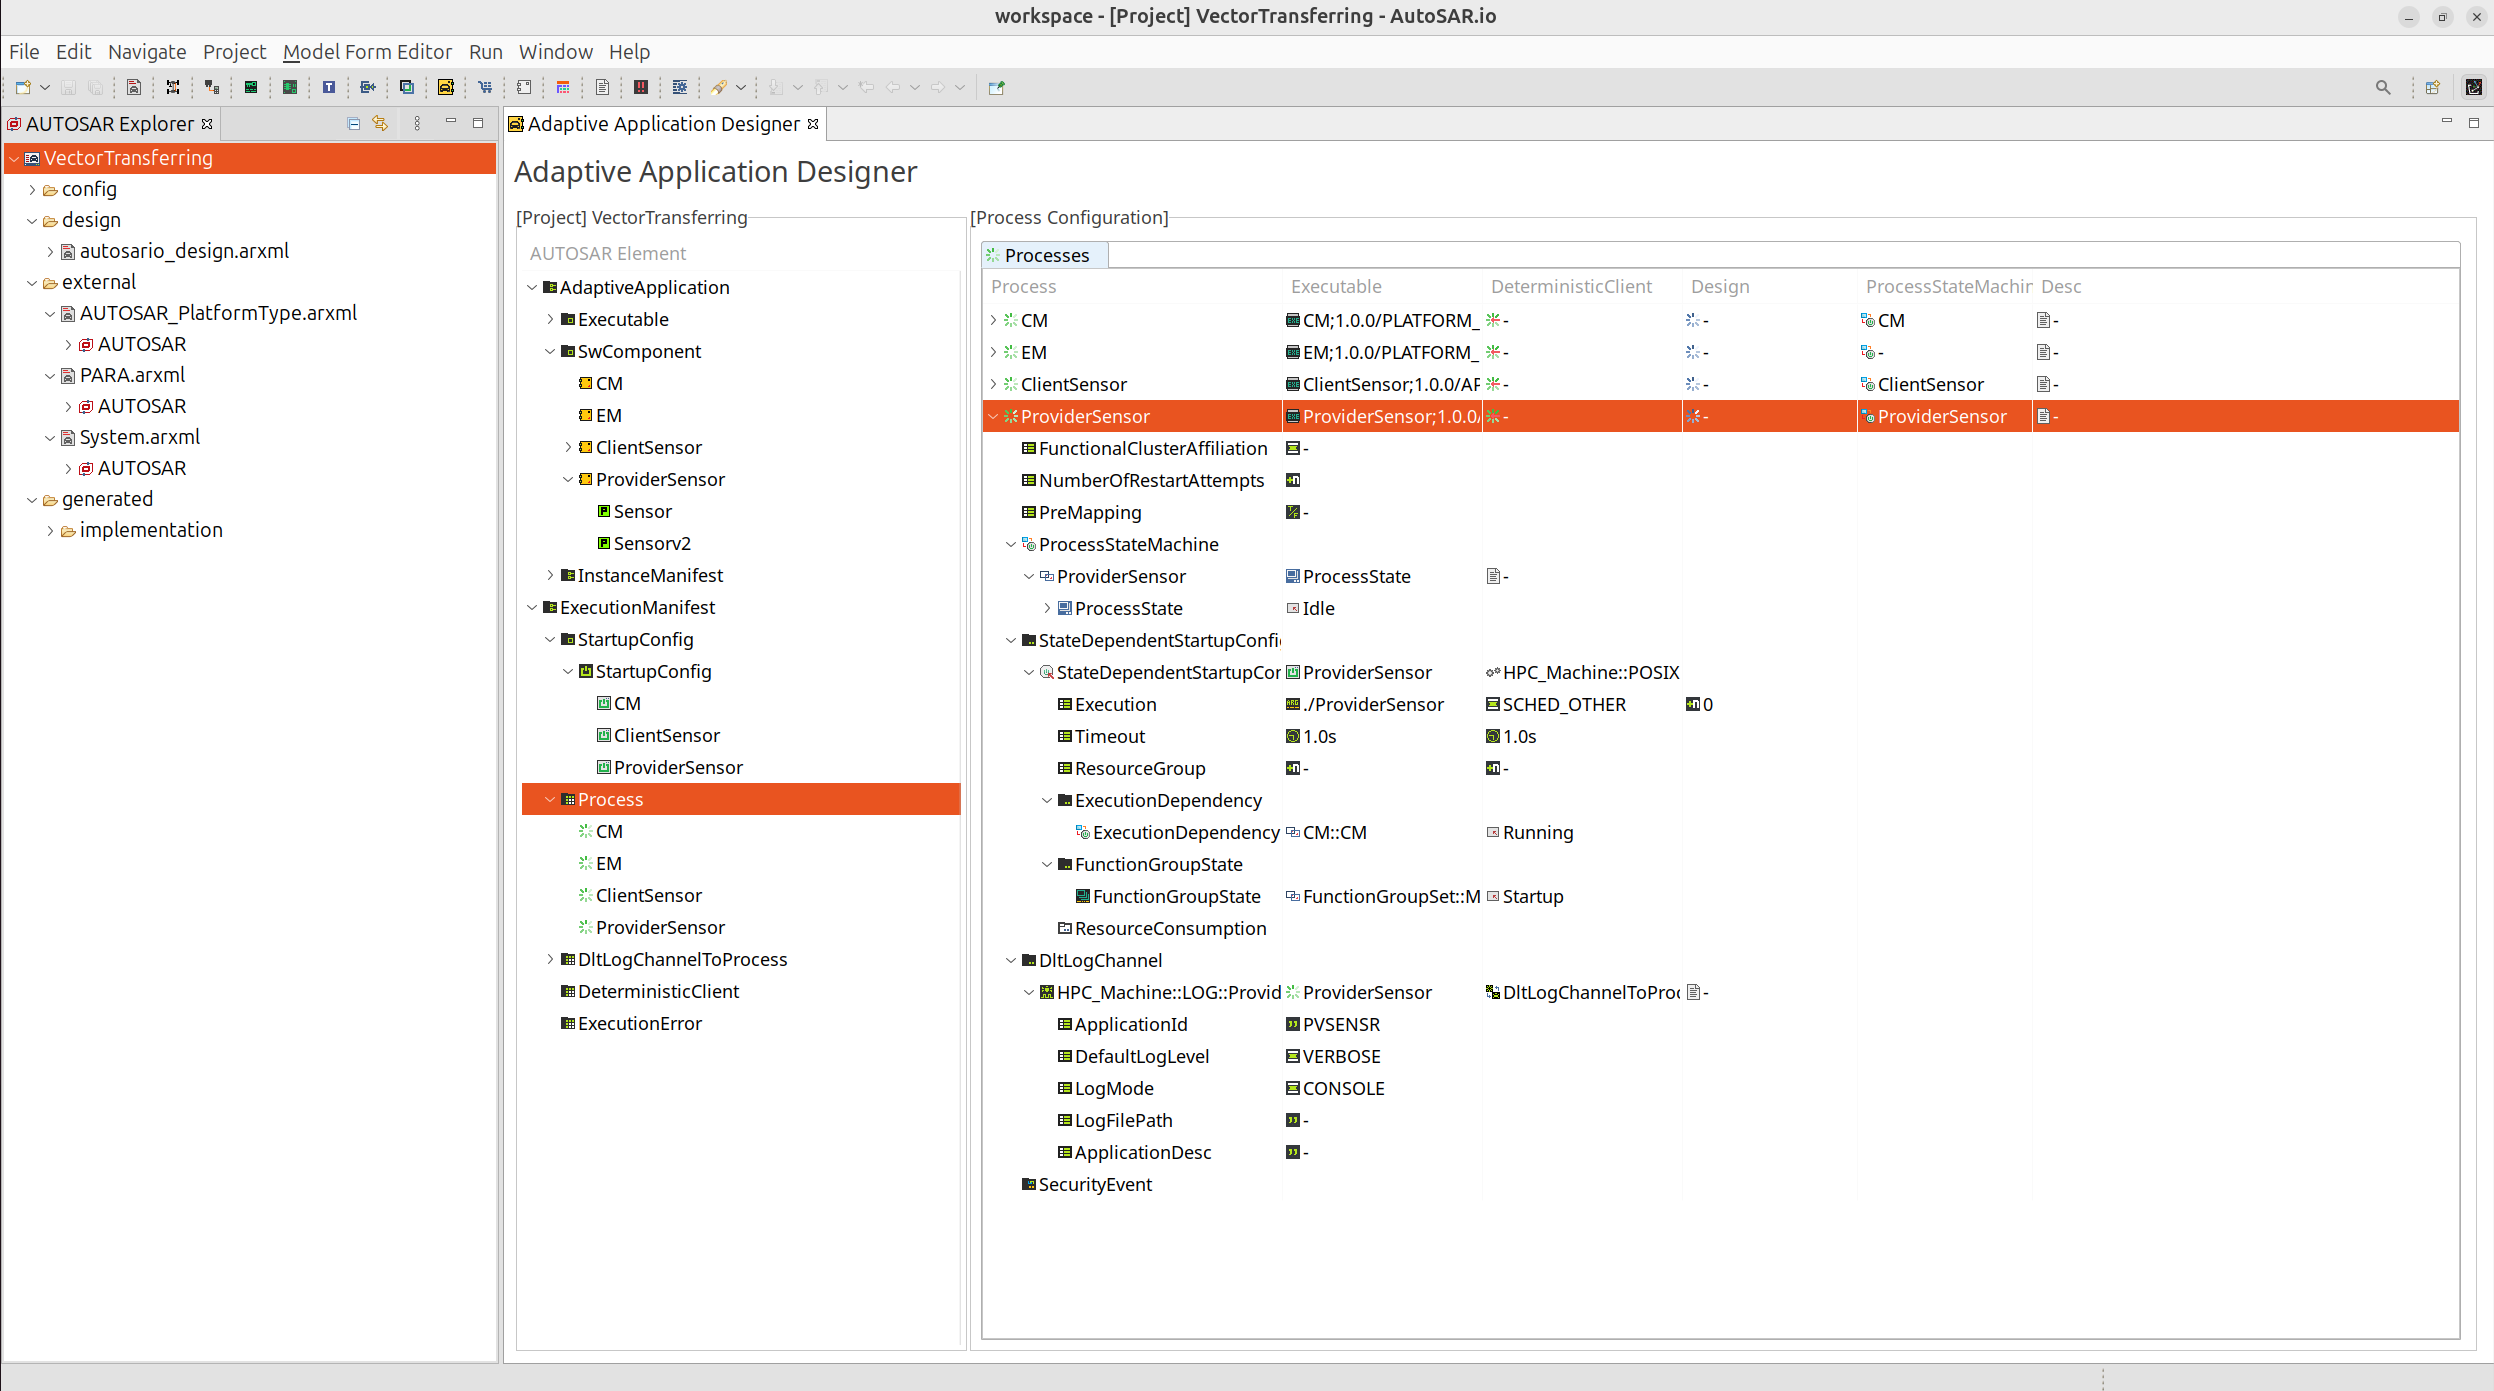
\includegraphics[width=0.75\textwidth]{Images/chap3/image_methodology/applicationDesign/configureProviderProcess.png}
    \vspace{0.5cm}
    \caption{Configuration of Provider Application Process}
    \label{fig:app_provider_process_configuration}
\end{figure}

As illustrated in Figure~\ref{fig:app_provider_process_configuration}, the provider application process is configured by linking the \texttt{ProviderSensor} executable to a dedicated process entity. This step specifies process level attributes such as restart policy, execution dependency, and state machine association, which together describe how the provider behaves during runtime transitions. The configuration clarifies the provider’s role in the execution flow and its dependency on platform level services.

% Configure Client Application Process
\begin{figure}[H]
    \centering
    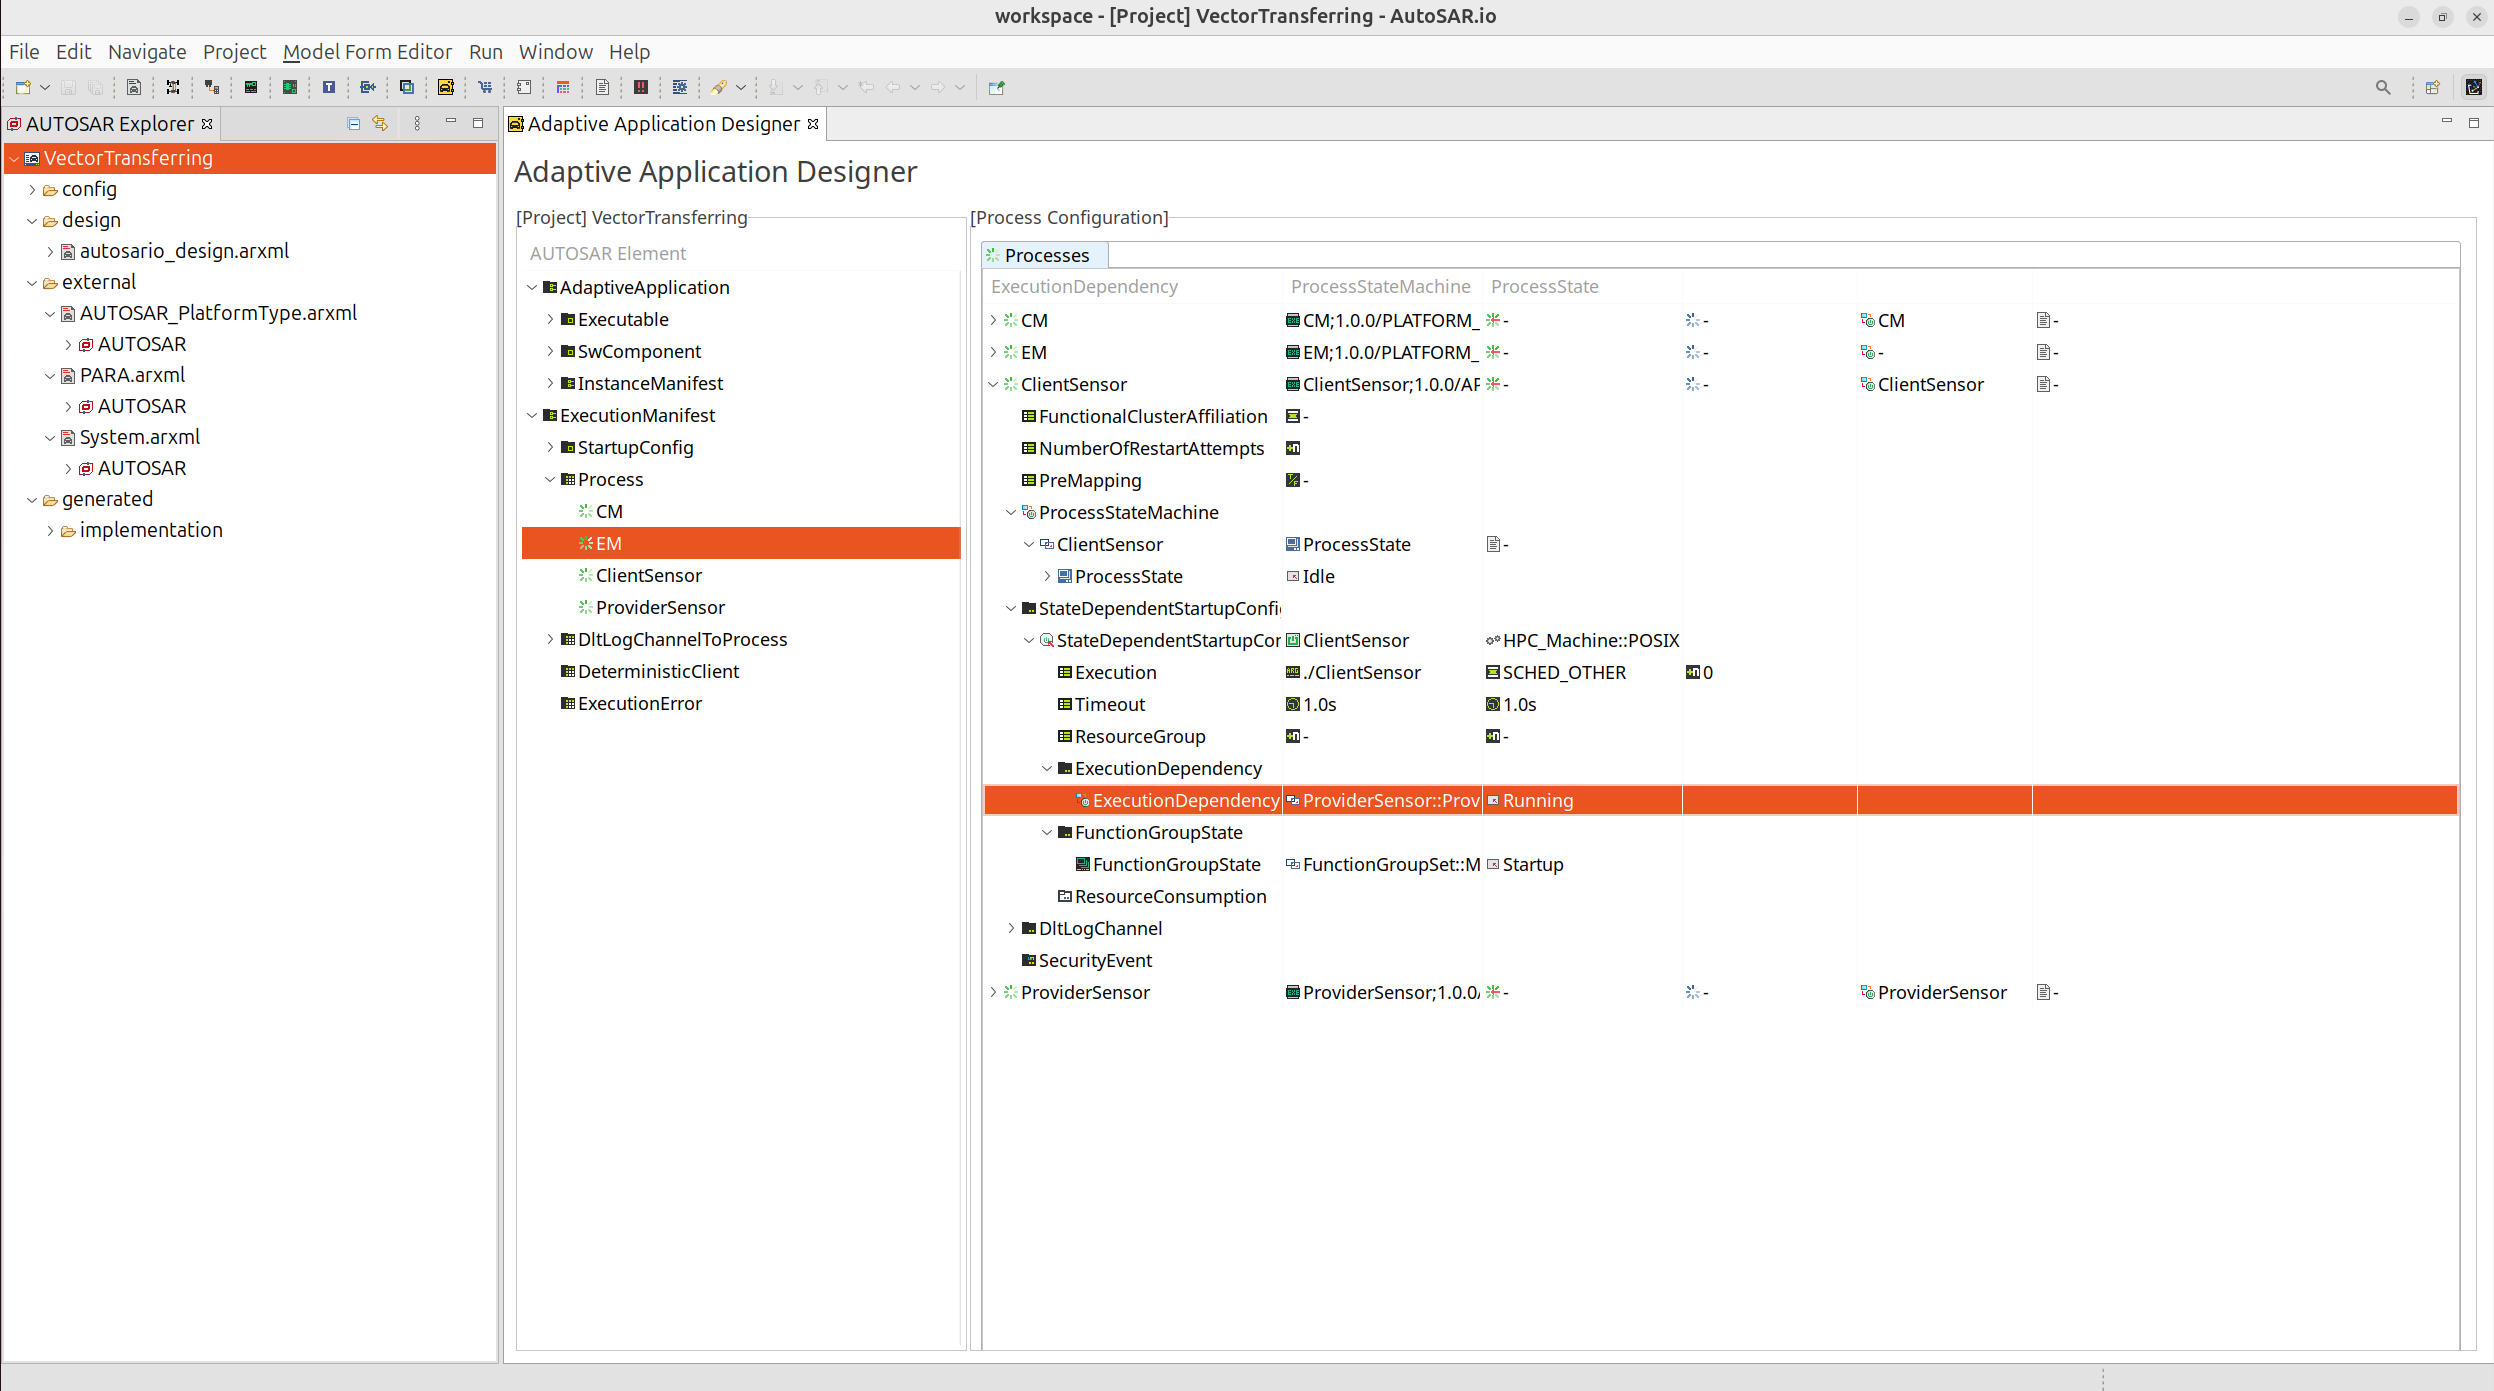
\includegraphics[width=0.75\textwidth]{Images/chap3/image_methodology/applicationDesign/configureClientProcess.png}
    \vspace{0.5cm}
    \caption{Configuration of Client Application Process}
    \label{fig:app_client_process_configuration}
\end{figure}

Figure~\ref{fig:app_client_process_configuration} shows a similar setup for the client application, where the \texttt{ClientSensor} executable is bound to its own process instance. Here, execution states and startup dependencies are defined to ensure that the client is activated only when required conditions are satisfied. This separation at the process level improves modularity and allows independent management of client and provider lifecycles.

% Map Application Processes to Target Machine
\begin{figure}[H]
    \centering
    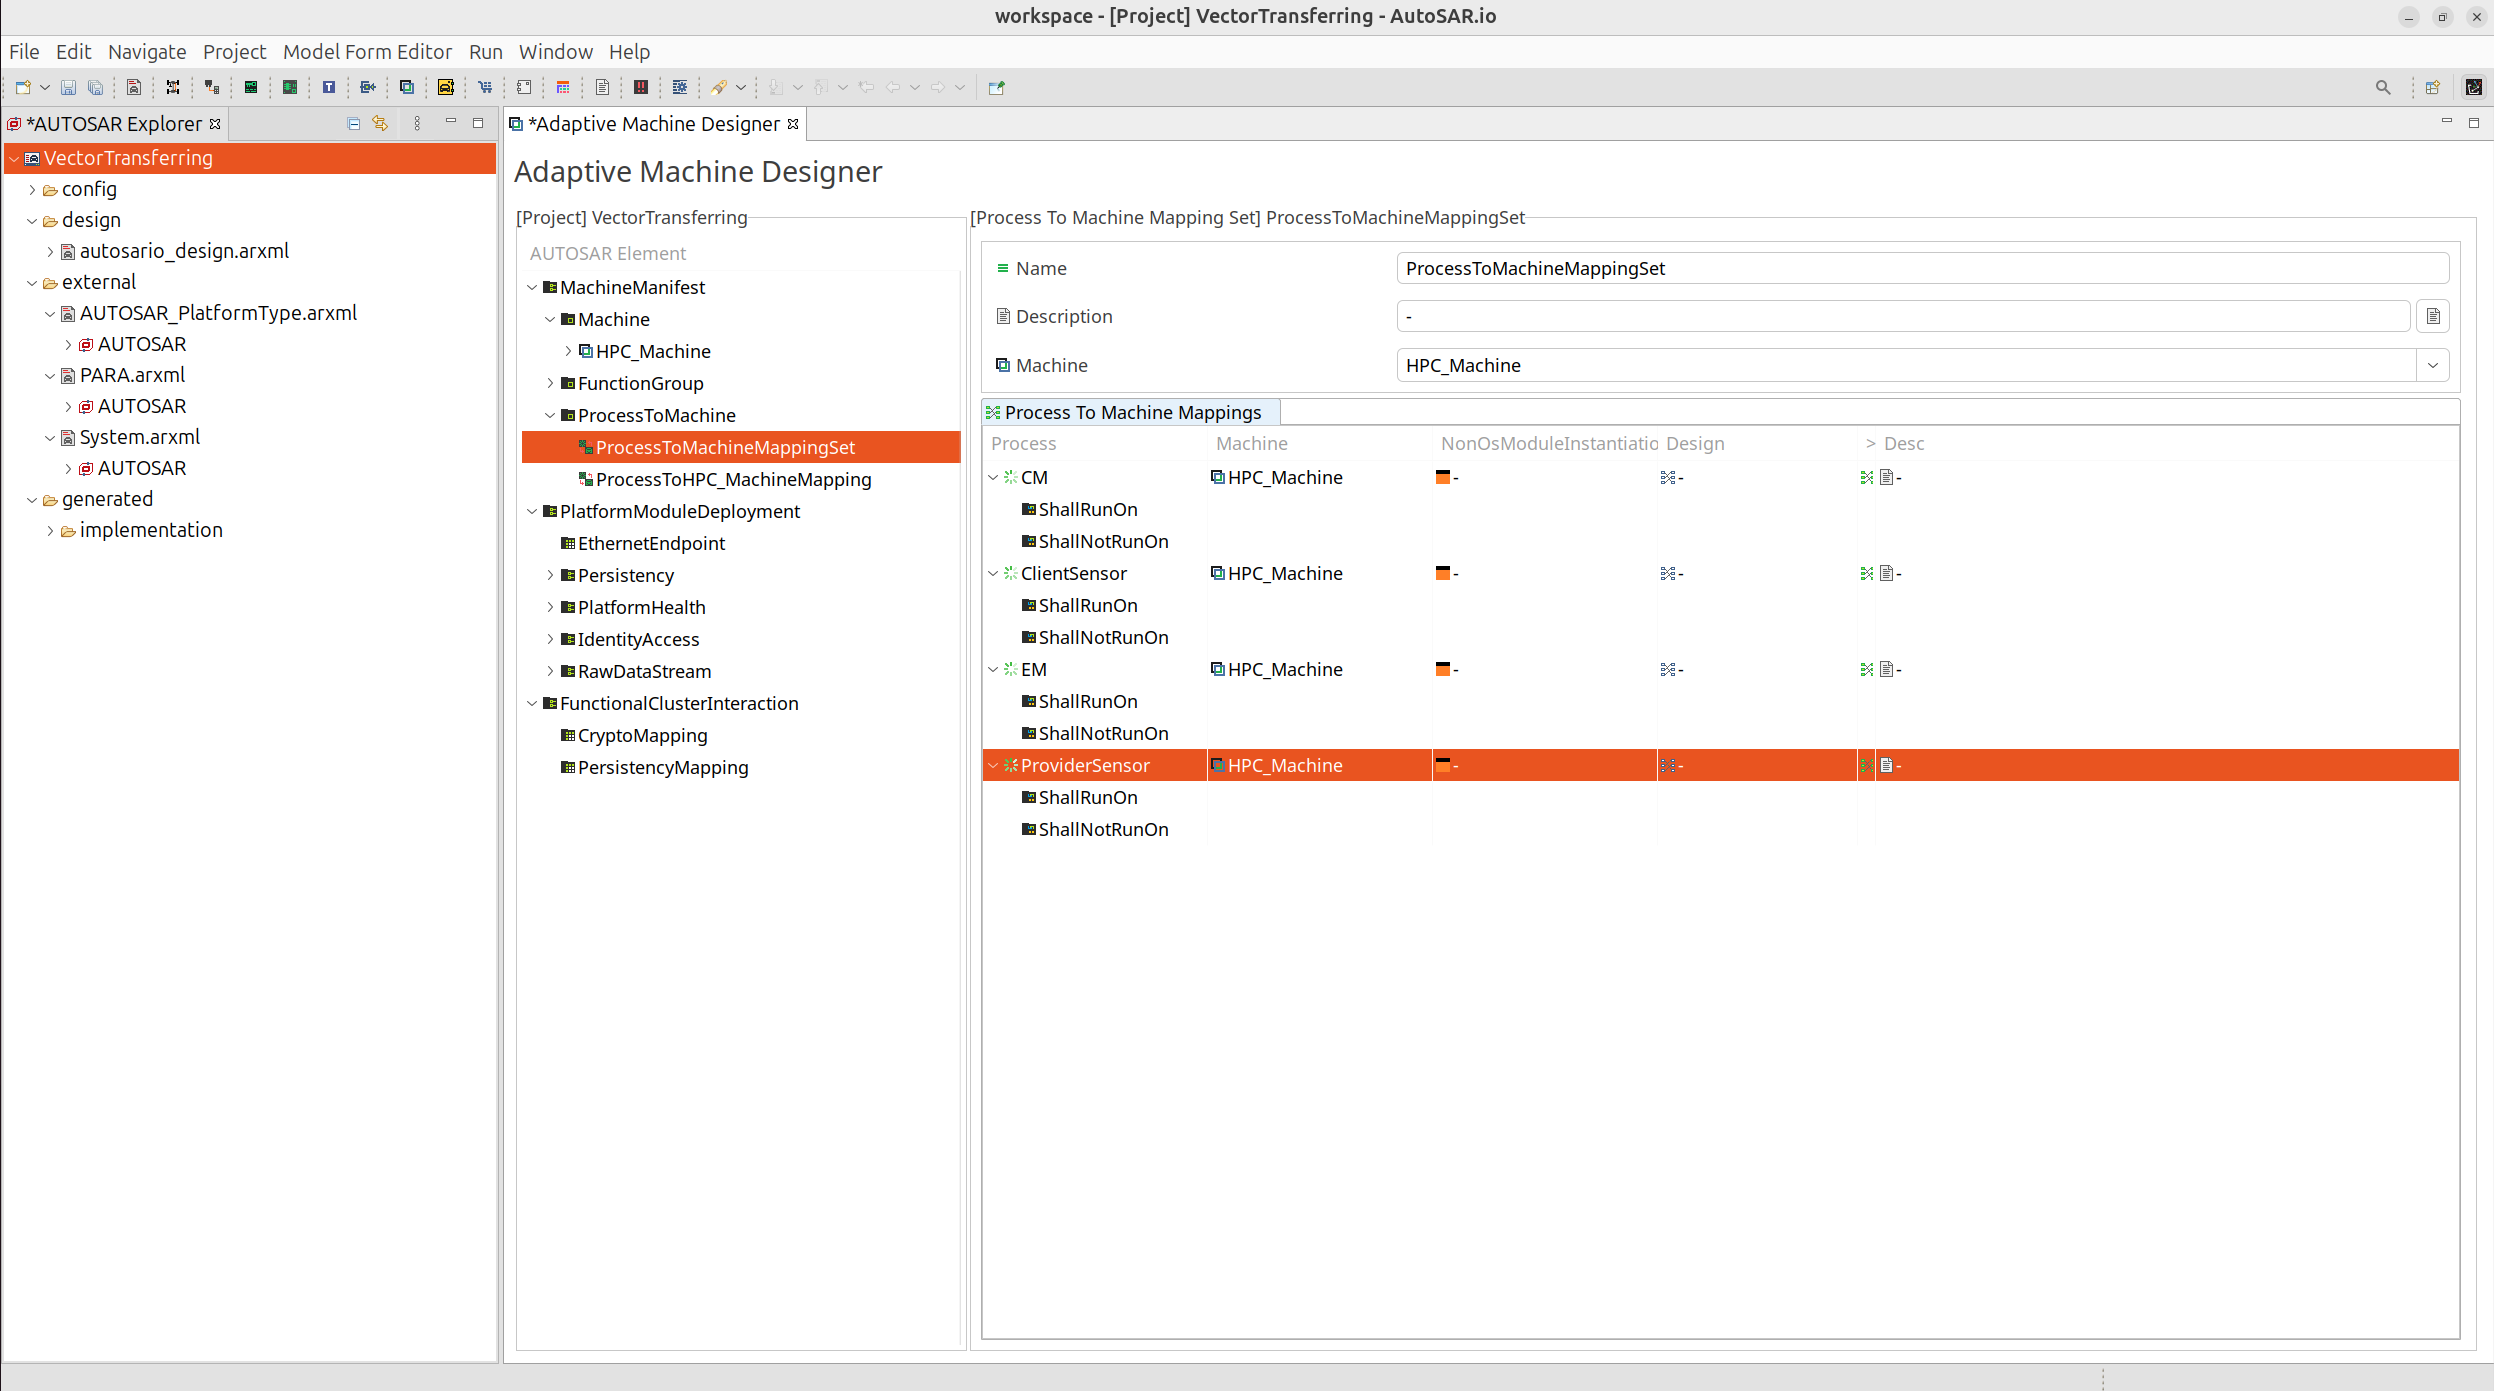
\includegraphics[width=0.75\textwidth]{Images/chap3/image_methodology/applicationDesign/mappingProcesstoMachine.png}
    \vspace{0.5cm}
    \caption{Mapping Application Processes to Target Machine}
    \label{fig:app_process_machine_mapping}
\end{figure}

Finally, Figure~\ref{fig:app_process_machine_mapping} presents the process-to-machine mapping defined in the Adaptive Machine Designer. In this step, all application processes, including \texttt{CM}, \texttt{EM}, \texttt{ClientSensor}, and \texttt{ProviderSensor}, are explicitly assigned to the target \texttt{HPC\_Machine}. This mapping determines the physical execution location of each process and establishes the final deployment relationship between the adaptive applications and the underlying hardware platform.

By consolidating all processes onto a single machine, the configuration ensures a coherent execution environment and simplifies resource management during runtime. This step completes the application deployment workflow by bridging the gap between application-level process definitions and machine-level execution, enabling the Adaptive AUTOSAR runtime to launch and supervise each process according to the previously defined startup, scheduling, and communication configurations.

\subsubsection{Generating Code and Manifest Files}
After completing the configuration steps at the machine, service, and application levels, the Autosar.io tool supports automatic generation of implementation artifacts through the PARA Generator. This generator collects all previously defined models, including Machine Manifests, service definitions, service instances, and application processes, and transforms them into deployable outputs that conform to the Adaptive AUTOSAR specification. By doing so, the tool ensures that the system configuration remains consistent from design time to implementation.

\begin{figure}[H]
    \centering
    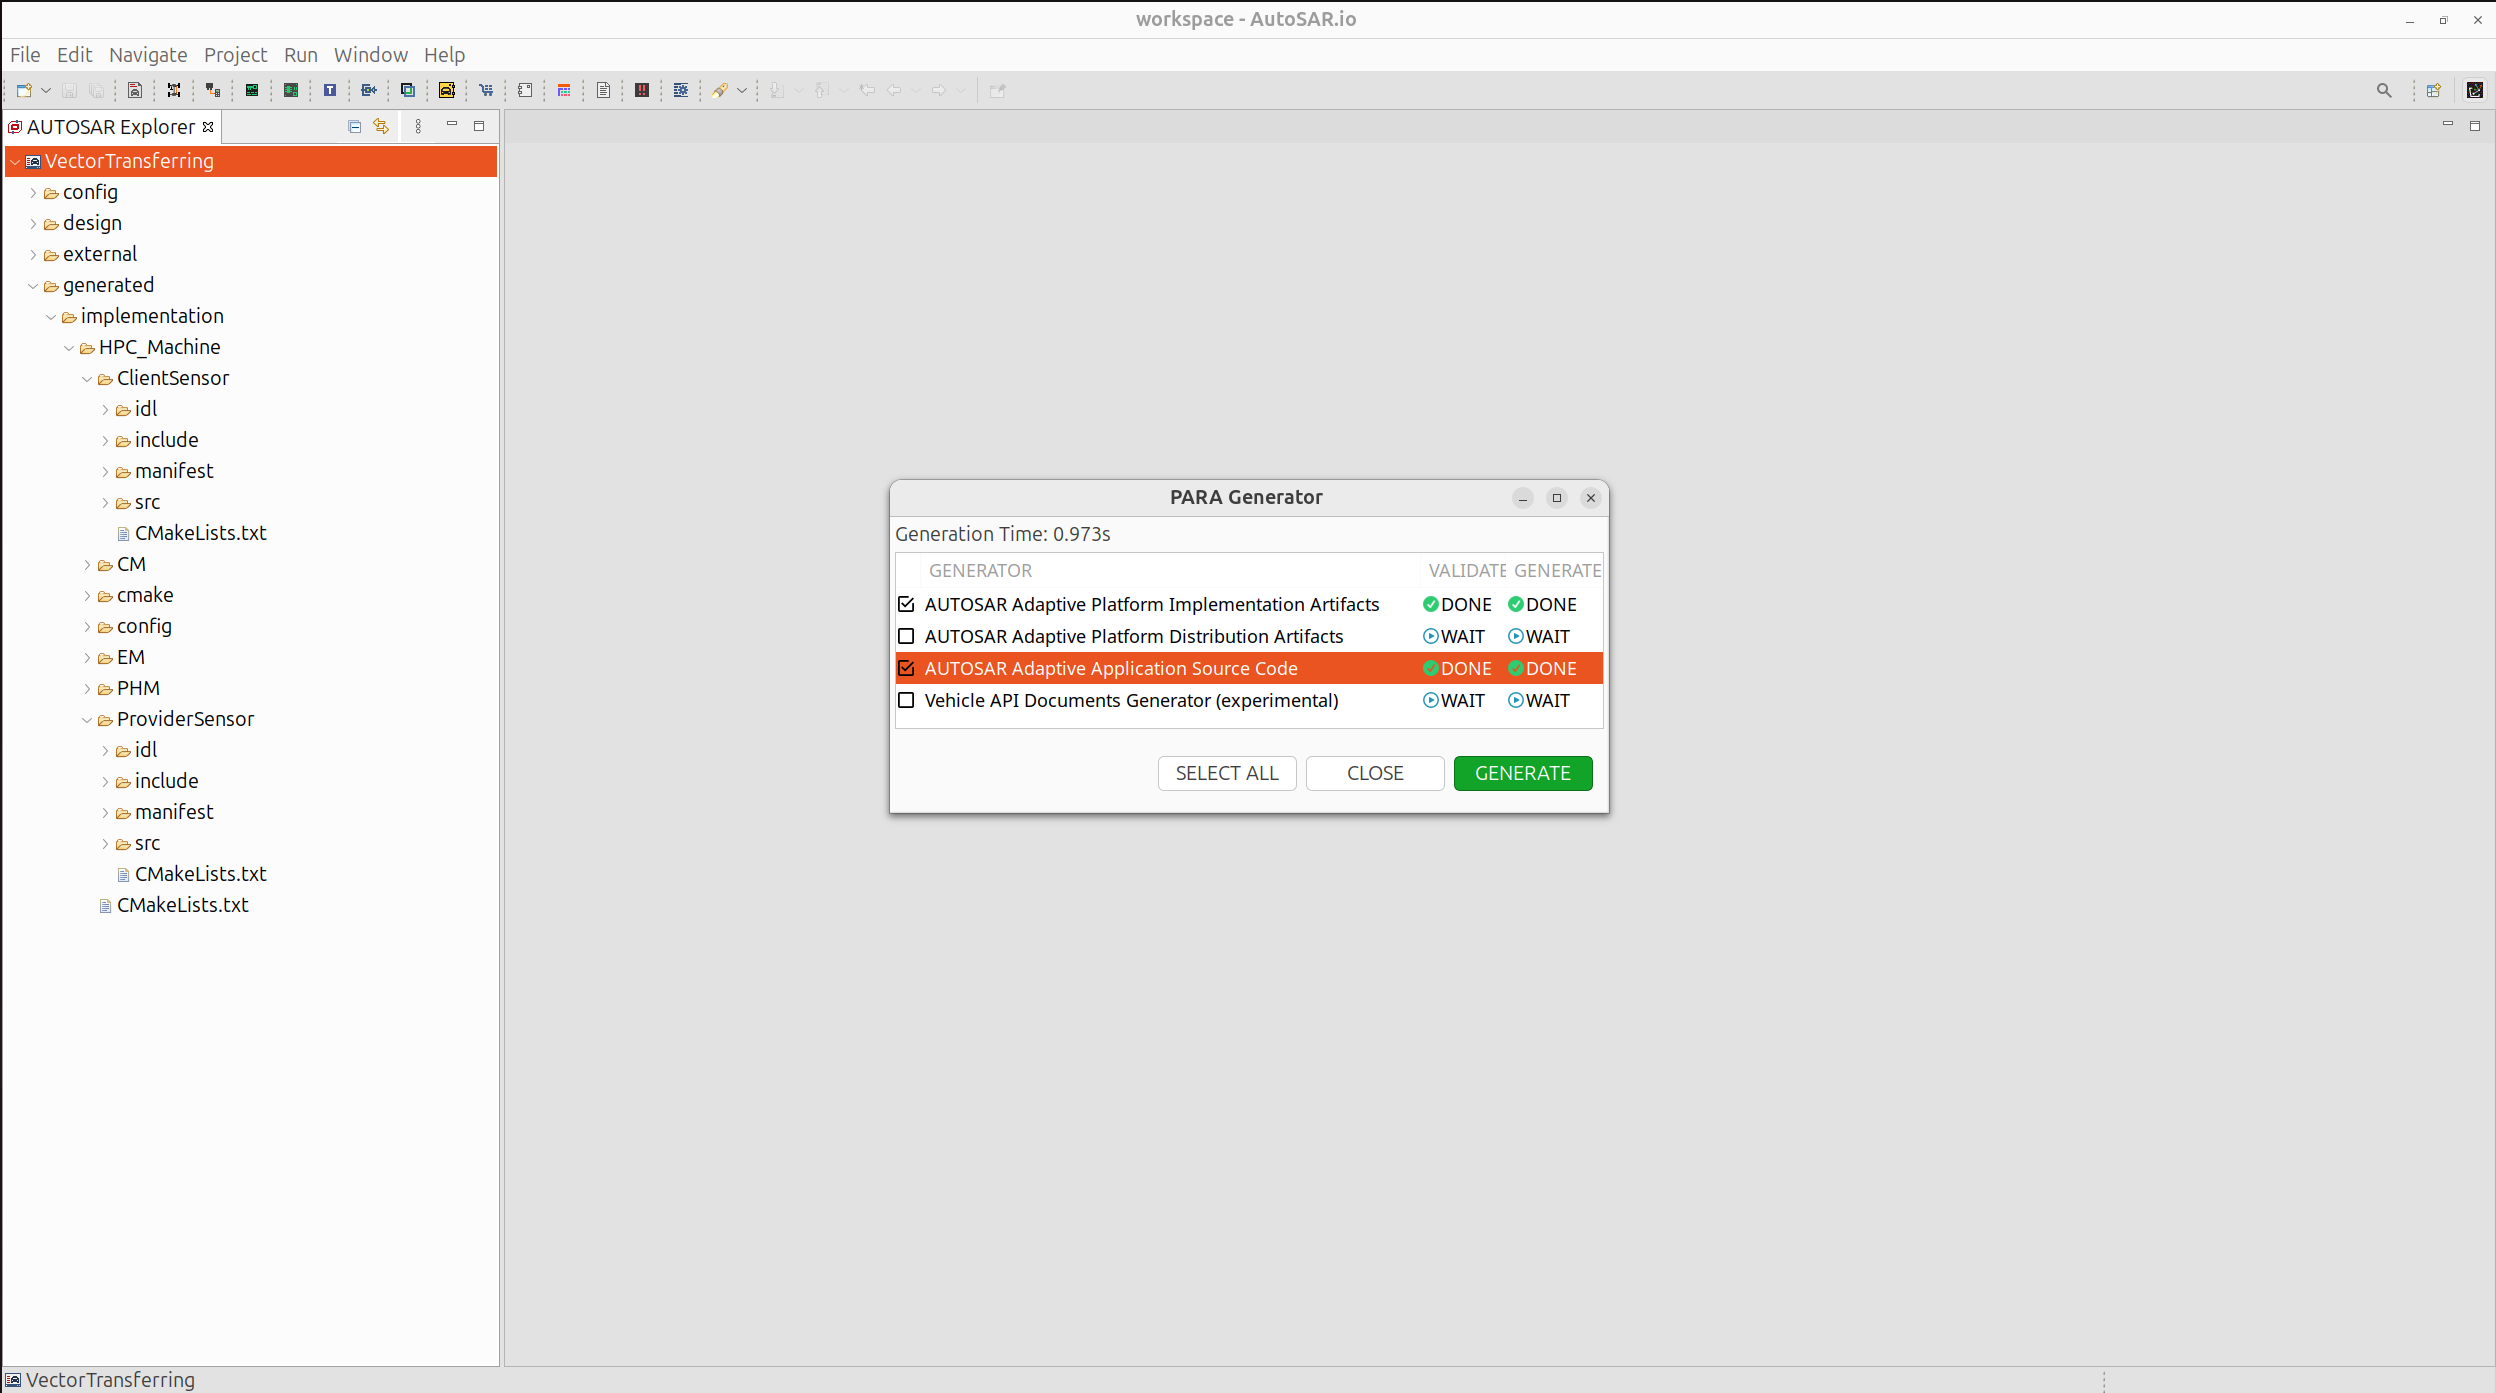
\includegraphics[width=0.75\textwidth]{Images/chap3/generating.png}
    \vspace{0.5cm}
    \caption{Generating Code and ARXML Files}
    \label{fig:code_generation}
\end{figure}

As illustrated in Figure~\ref{fig:code_generation}, the PARA Generator allows users to selectively generate different categories of artifacts, such as Adaptive Application source code, platform configuration files, and manifest descriptions. The generation process produces AUTOSAR compliant ARXML files together with structured C++ source code for each executable. These outputs follow a standardized directory layout, which simplifies subsequent build and integration steps.

Through this automated generation mechanism, Autosar.io bridges the gap between high level system modeling and concrete software artifacts. The generated code and configuration files serve as a reliable foundation for compilation, deployment, and runtime execution. This approach reduces manual errors, improves traceability, and supports a smooth transition from configuration to system integration in the Adaptive AUTOSAR development workflow.
